\باب{تعددی ردعمل}
گزشتہ بابوں میں ہم \عددی{RLC} ادوار کو حل کر چکے ہیں جہاں تعدد غیر متغیر تھی۔اس باب میں تعدد تبدیل کرتے ہوئے ادوار کا ردعمل بالمقابل تعدد دیکھا جائے گا۔آئیں شروع میں سادہ ترین پرزوں کا تعددی رد عمل دیکھیں۔سادہ ترین پرزے  مزاحمت، امالہ اور برق گیر ہیں۔تعددی رد عمل دیکھتے ہوئے سائن نما اشارات زیر استعمال لائے جائیں گے۔ 

شکل \حوالہ{شکل_تعددی_مزاحمتی_ردعمل}-الف میں مزاحمت دکھایا گیا ہے۔مزاحت کی رکاوٹ درج ذیل ہے۔
\begin{align}
Z_R=R\phase{0^{\circ}}
\end{align}
یوں مزاحمت کی رکاوٹ پر تعدد \عددی{\omega} کا کوئی اثر نہیں پایا جاتا۔مزاحمت کے رکاوٹ کی حتمی قیمت \عددی{\abs{\bZ_R}} تمام تعدد پر \عددی{R} کے برابر ہے جبکہ اس کا زاویائی ہٹاو \عددی{\phase{\bZ_R}} تمام تعدد پر صفر درجے رہتا ہے۔یہ حقائق شکل \حوالہ{شکل_تعددی_مزاحمتی_ردعمل}-ب اور شکل \حوالہ{شکل_تعددی_مزاحمتی_ردعمل}-پ میں دکھائے گئے ہیں۔
\begin{figure}
\centering
\begin{subfigure}{1\textwidth}
\centering
\begin{tikzpicture}
\draw(0,0) to [short,o-]++(\x,0) to [resistor,l_={$R$}]++(0,\y) to [short,-o]++(-\x,0);
\draw[stealth-](\x/4,\y/2)--++(-\x/4,0)--++(0,-\y/8)node[below]{$\bZ_R$};
\end{tikzpicture}
\caption*{(الف) مزاحمت کی رکاوٹ۔}
\end{subfigure}
\begin{subfigure}{0.5\textwidth}
\centering
\begin{tikzpicture}
\begin{axis}[kStyleCircuitsA,name=ka,small,
,xlabel=$\omega$,ylabel=$\abs{\bZ_R}$,ytick={0.5},yticklabels={$R$},ymax=0.75,ymin=0,xmin=0,xtick=\empty]
\addplot[domain=0:3,samples=2]{0.5};
\end{axis}%
\end{tikzpicture}%
\caption*{(ب) مزاحمتی رکاوٹ کی حتمی قیمت بالمقابل تعدد۔}
\end{subfigure}%
\begin{subfigure}{0.5\textwidth}
\centering
\begin{tikzpicture}
\begin{axis}[kStyleCircuitsA,name=ka,small,
,xlabel=$\omega$,ylabel=$\phase{\bZ_R}$,ytick={0.25},yticklabels={$0^{\circ}$},ymax=0.75,ymin=0,xmin=0,xtick=\empty]
\addplot[domain=0:3,samples=2]{0.25};
\end{axis}
\end{tikzpicture}%
\caption*{(پ) مزاحمتی رکاوٹ کا زاویہ بالمقابل تعدد۔}
\end{subfigure}%
\caption{مزاحمتی رکاوٹ کا تعدد ردعمل۔}
\label{شکل_تعددی_مزاحمتی_ردعمل}
\end{figure}

امالہ گیر کو شکل \حوالہ{شکل_تعددی_امالی_ردعمل}-الف میں دکھایا گیا ہے۔امالہ گیر کی رکاوٹ درج ذیل ہے۔
\begin{align}
\bZ_L&=j\omega L=\omega L\phase{90^{\circ}}
\end{align}
اس طرح امالہ گیر کے رکاوٹ کی حتمی قیمت تعدد بڑھانے سے بڑھتی ہے۔رکاوٹ کی مقدار کا تعدد کے ساتھ راست تنابی رشتہ ہے۔
\begin{align}
\abs{\bZ_L}=\omega L
\end{align}
صفر تعدد پر امالہ گیر کی رکاوٹ \عددی{\SI{0}{\ohm}} ہو جاتی ہے اور یہ قصر دور خاصیت رکھتا ہے جبکہ لامتناہی تعدد پر رکاوٹ کی مقدار لامتناہی ہو جاتی ہے اور امالہ گیر بطور کھلا دور عمل کرتا ہے۔امالی رکاوٹ کا زاویہ تمام تعدد پر \عددی{90^{\circ}} رہتا ہے۔
\begin{align}
\phase{\bZ_L}=90^{\circ}
\end{align}
شکل \حوالہ{شکل_تعددی_امالی_ردعمل}-ب اور شکل \حوالہ{شکل_تعددی_امالی_ردعمل}-پ میں ان حقائق کو دکھایا گیا ہے۔
\begin{figure}
\centering
\begin{subfigure}{1\textwidth}
\centering
\begin{tikzpicture}
\draw(0,0) to [short,o-]++(\x,0) to [inductor,l_={$L$}]++(0,\y) to [short,-o]++(-\x,0);
\draw[stealth-](\x/4,\y/2)--++(-\x/4,0)--++(0,-\y/8)node[below]{$\bZ_L$};
\end{tikzpicture}
\caption*{(الف) امالہ گیر کی رکاوٹ۔}
\end{subfigure}
\begin{subfigure}{0.5\textwidth}
\centering
\begin{tikzpicture}
\begin{axis}[kStyleCircuitsA,name=ka,small,
,xlabel=$\omega$,ylabel=$\abs{\bZ_L}$,ytick=\empty,ymin=0,xmin=0,xtick=\empty]
\addplot[domain=0:10,samples=10]{0.5*x};
\end{axis}%
\end{tikzpicture}%
\caption*{(ب) امالی رکاوٹ کی حتمی قیمت بالمقابل تعدد۔}
\end{subfigure}%
\begin{subfigure}{0.5\textwidth}
\centering
\begin{tikzpicture}
\begin{axis}[kStyleCircuitsA,name=ka,small,
,xlabel=$\omega$,ylabel=$\phase{\bZ_L}$,ytick={0.5},yticklabels={$90^{\circ}$},ymax=0.75,ymin=0,xmin=0,xtick=\empty]
\addplot[domain=0:3,samples=2]{0.5};
\end{axis}
\end{tikzpicture}%
\caption*{(پ) امالی رکاوٹ کا زاویہ بالمقابل تعدد۔}
\end{subfigure}%
\caption{امالی رکاوٹ کا تعدد ردعمل۔}
\label{شکل_تعددی_امالی_ردعمل}
\end{figure}

برق گیر کو شکل \حوالہ{شکل_تعددی_برق_گیری_ردعمل}-الف میں دکھایا گیا ہے۔برق گیر کی رکاوٹ درج ذیل ہے۔
\begin{align}
\bZ_C=\frac{1}{j\omega C}=\frac{1}{\omega C}\phase{-90^{\circ}}
\end{align}
اس طرح برق گیر کے رکاوٹ کی مقدار کا تعدد کے ساتھ بالعکس متناسب کا رشتہ ہے جبکہ اس کا زاویہ تمام تعدد پر \عددی{-90^{\circ}} رہتا ہے۔
\begin{align}
\abs{\bZ_C}&=\frac{1}{\omega C}\\
\phase{\bZ_C}&=-90^{\circ}
\end{align}
ان تعلقات کو شکل \حوالہ{شکل_تعددی_برق_گیری_ردعمل}-ب اور شکل \حوالہ{شکل_تعددی_برق_گیری_ردعمل}-پ میں دکھایا گیا ہے۔ صفر تعدد پر برق گیر کی رکاوٹ لامتناہی ہو جاتی ہے لہٰذا یہ بطور کھلا دور عمل کرتا ہے جبکہ لامتناہی تعدد پر رکاوٹ کی مقدار صفر ہو جاتی ہے اور یہ قصر دور کردار ادا کرتا ہے۔
\begin{figure}
\centering
\begin{subfigure}{1\textwidth}
\centering
\begin{tikzpicture}
\draw(0,0) to [short,o-]++(\x,0) to [capacitor,l_={$C$}]++(0,\y) to [short,-o]++(-\x,0);
\draw[stealth-](\x/4,\y/2)--++(-\x/4,0)--++(0,-\y/8)node[below]{$\bZ_C$};
\end{tikzpicture}
\caption*{(الف) برق گیر کی رکاوٹ۔}
\end{subfigure}
\begin{subfigure}{0.5\textwidth}
\centering
\begin{tikzpicture}
\begin{axis}[kStyleCircuitsA,name=ka,small,
,xlabel=$\omega$,ylabel=$\abs{\bZ_C}$,ytick=\empty,ymin=0,xmin=0,xtick=\empty]
\addplot[domain=10:60,samples=100]{1/(0.5*x)};
\end{axis}%
\end{tikzpicture}%
\caption*{(ب) برق گیر رکاوٹ کی حتمی قیمت بالمقابل تعدد۔}
\end{subfigure}%
\begin{subfigure}{0.5\textwidth}
\centering
\begin{tikzpicture}
\begin{axis}[kStyleCircuitsA,name=ka,small,
,xlabel=$\omega$,ylabel=$\phase{\bZ_C}$,ytick={0.5},yticklabels={$-90^{\circ}$},ymax=0.75,xmin=0,xtick=\empty]
\addplot[domain=0:3,samples=2]{0.5};
\end{axis}
\end{tikzpicture}%
\caption*{(پ) برق گیر رکاوٹ کا زاویہ بالمقابل تعدد۔}
\end{subfigure}%
\caption{برق گیر رکاوٹ کا تعدد ردعمل۔}
\label{شکل_تعددی_برق_گیری_ردعمل}
\end{figure}

سادہ ترین پرزوں کو نپٹانے کے بعد ذرہ مشکل ادوار دیکھتے ہیں۔شکل میں مزاحمت، امالہ گیر اور برق گیر سلسلہ وار جڑے دکھائے گئے ہیں۔ان کی کل رکاوٹ \عددی{\bZ_s} لکھتے ہیں
\begin{align*}
\bZ_s&=\bZ_R+\bZ_L+\bZ_C\\
&=R+j\omega L+\frac{1}{j\omega C}\\
&=R+j\left(\omega L-\frac{1}{\omega C}\right)
\end{align*}
اس تفاعل کو شکل \حوالہ{شکل_تعددی_مزاحمت_املہ_برق_گیر_سلسلہ_وار_ردعمل}-ب اور شکل \حوالہ{شکل_تعددی_مزاحمت_املہ_برق_گیر_سلسلہ_وار_ردعمل}-پ میں دکھایا گیا ہے۔
%
\begin{figure}
\centering
\begin{subfigure}{1\textwidth}
\centering
\begin{tikzpicture}
\draw(0,0) to [resistor,o-,l={$R$}]++(\x,0) to [inductor,l={$L$}]++(\x,0) to  [capacitor,l={$C$}]++(0,-\y) to [short,-o]++(-2*\x,0);
\draw[stealth-](\x/4,-\y/2)--++(-\x/4,0)--++(0,-\y/8)node[below]{$\bZ_s$};
\end{tikzpicture}
\caption*{(الف) سلسلہ وار دور۔}
\end{subfigure}
\begin{subfigure}{0.5\textwidth}
\centering
\begin{tikzpicture}
\begin{axis}[kStyleCircuitsA,name=ka,small,
,xlabel=$\omega$,ylabel=$\abs{\bZ_C}$,ytick=\empty,ymin=0,xmin=0,xtick={1},xticklabels={$\omega_0$}]
\addplot[domain=0:5,samples=100]{sqrt((1-x^2)^2+x^2)/x};
\end{axis}%
\end{tikzpicture}%
\caption*{(ب) مقدار بالمقابل تعدد۔}
\end{subfigure}%
\begin{subfigure}{0.5\textwidth}
\centering
\begin{tikzpicture}
\begin{axis}[kStyleCircuitsA,name=ka,small,
,xlabel=$\omega$,ylabel=$\phase{\bZ_C}$,ytick={-90,0,90},yticklabels={$-90^{\circ}$,$0^{\circ}$,$90^{\circ}$},ymax=120,xmin=0,xtick={1},xticklabels={$\omega_0$}]
\addplot[domain=0.01:3,samples=100]{atan(x-1/x)};
\end{axis}
\end{tikzpicture}%
\caption*{(پ) زاویہ بالمقابل تعدد۔}
\end{subfigure}%
\caption{سلسلہ وار جڑے مزاحمت، امالہ گیر اور برق گیر کا تعدد ردعمل۔}
\label{شکل_تعددی_مزاحمت_املہ_برق_گیر_سلسلہ_وار_ردعمل}
\end{figure}
%======================
\ابتدا{مثال}\شناخت{مثال_تعددی_بوڈا_خط_مزاحمت_امالہ_برق_گیر_رو_الف}
شکل \حوالہ{شکل_تعددی_بوڈا_خط_مزاحمت_امالہ_برق_گیر_رو_الف}-الف میں مزاحمت پر دباو حاصل کریں۔اس کے مقدار بالمقابل تعدد اور زاویہ بالمقابل تعدد کے خط کھینچیں۔
\begin{figure}
\centering
\begin{subfigure}{1\textwidth}
\centering
\begin{tikzpicture}[american voltages]
\draw(0,0) to [capacitor,l={$\SI{4}{\milli\farad}$}]++(\x,0) to [inductor,l={$\SI{0.15}{\henry}$}]++(\x,0) to  [resistor,l={$\SI{10}{\ohm}$},v={$\hat{V}_R$}]++(0,-\y) to [short]++(-2*\x,0) to [american voltage source,l={$20\phase{0^{\circ}}\,\si{\volt}$}]++(0,\y);
\end{tikzpicture}
\caption*{(الف)}
\end{subfigure}
\begin{subfigure}{1\textwidth}
\centering
\includegraphics{figFreqMagRLCvoltA}
\caption*{(ب) مقدار بالمقابل تعدد کا خط۔}
\end{subfigure}
\begin{subfigure}{1\textwidth}
\centering
\includegraphics{figFreqPhaseRLCvoltA}
\caption*{(پ) زاویہ بالمقابل تعدد کا خط۔}
\end{subfigure}
\caption{مثال \حوالہ{مثال_تعددی_بوڈا_خط_مزاحمت_امالہ_برق_گیر_رو_الف} کا دور۔}
\label{شکل_تعددی_بوڈا_خط_مزاحمت_امالہ_برق_گیر_رو_الف}
\end{figure}

حل:دور سے مزاحمت کا دباو درج ذیل لکھا جا سکتا ہے
\begin{align*}
\hat{V}_R=\frac{(4)(20\phase{0^{\circ}})}{4+j(2\pi f 0.15-\frac{1}{2\pi f 0.004})}
\end{align*}
جو مخلوط تفاعل ہے۔اس کی حتمی مقدار \عددی{\hat{V}_R} بالمقابل تعدد \عددی{f} کو شکل-ب میں دکھایا گیا ہے۔اس ترسیم میں دونوں محور کی پیمائش \اصطلاح{لاگ}\فرہنگ{لاگ}\حاشیہب{log}\فرہنگ{log} میں ہے۔اس طرز کے ترسیم کو \اصطلاح{لاگ لاگ}\فرہنگ{لاگ لاگ!ترسیم}\فرہنگ{ترسیم!لاگ لاگ}\حاشیہب{log-log}\فرہنگ{log-log!graph}\فرہنگ{graph!log-log} ترسیم کہا جاتا  ہے۔مقدار بالمقابل تعدد کے خط عموماً لاگ لاگ محور پر دکھائے جاتے ہیں۔ زاویہ دباو \عددی{\phase{\hat{V}_R}} بالمقابل تعدد کو شکل-پ میں \اصطلاح{نیم لاگ}\فرہنگ{نیم لاگ!ترسیم}\فرہنگ{ترسیم!نیم لاگ}\حاشیہب{semilog}\فرہنگ{semilog!axis}\فرہنگ{axis!semilog} محور پر دکھایا گیا ہے۔کم تعدد پر دباو کا زاویہ \عددی{+90^{\circ}} جبکہ بلند تعدد پر زاویہ \عددی{-90^{\circ}} ہے۔
\انتہا{مثال}
%========================

یہاں لاگ لاگ اور نیم لاگ محور پر قیمتیں پڑھنا سیکھ لیں چونکہ اس باب میں انہیں کا استعمال ہو گا۔یوں شکل \حوالہ{شکل_تعددی_بوڈا_خط_مزاحمت_امالہ_برق_گیر_رو_الف}-ب میں  حتمی مقدار کی چوٹی \عددی{10^1} یعنی دس ہرٹز پر پائی جاتی ہے۔یہ چوٹی \عددی{10^1} یعنی دس وولٹ کو ظاہر کرتی ہے۔اسی طرح \عددی{\SI{e2}{\hertz}} یعنی سو ہرٹز پر دباو تقریباً  \عددی{\SI{1.6}{\volt}} ہے۔

\اصطلاح{سمعی}\فرہنگ{سمعی}\حاشیہب{audio}\فرہنگ{audio} اشارات کو \اصطلاح{عددی صورت}\فرہنگ{عددی صورت}\حاشیہب{digital form}\فرہنگ{digital form} میں تبدیل کرتے ہوئے کمپیوٹر میں ذخیرہ کیا جاتا ہے۔ انہیں کو دوبارہ \اصطلاح{مماثل صورت}\فرہنگ{مماثل صورت}\حاشیہب{analog form}\فرہنگ{analog form} میں تبدیل کرتے ہوئے سنا جا سکتا ہے۔آئیں ان اشارات پر ایک مثال دیکھیں۔

کمپیوٹر سے حاصل موسیقی کے مماثلی اشارات کی چوٹی \عددی{\SI{1.5}{\volt}} ہے۔ ہم چاہتے ہیں کہ \اصطلاح{سمعی دباو ایمپلیفائر}\فرہنگ{ایمپلیفائر!سمعی}\فرہنگ{سمعی ایمپلیفائر}\حاشیہب{voltage amplifier}\فرہنگ{voltage!amplifier} استعمال کرتے ہوئے \عددی{\SI{8}{\ohm}} کے \اصطلاح{سپیکر}\فرہنگ{سپیکر}\حاشیہب{loud speaker}\فرہنگ{speaker} کو \عددی{\SI{10}{\watt}} طاقت فراہم کی جائے۔ان حقائق سے ایمپلیفائر کے داخلی مماثل اشارہ کی موثر قیمت حاصل کرتے ہیں۔
\begin{align*}
v_m=\frac{1.5}{\sqrt{2}}=\SI{1.061}{\volt}\,\rms
\end{align*}
طاقت کے کلیے \عددی{P=\tfrac{\VrmsS}{R}} سے آٹھ اوہم کے سپیکر کو دس واٹ طاقت کے لئے درکار موثر دباو حاصل کرتے ہیں۔
\begin{align*}
v_0=\sqrt{(10)(8)}=\SI{8.944}{\volt}\,\rms
\end{align*} 
یوں ایمپلیفائر کی درکار افزائش دباو درج ذیل ہے۔
\begin{align*}
A_v=\frac{v_0}{v_m}=\frac{8.944}{1.061}=\SI{8.43}{\volt\per\volt}
\end{align*}
شکل \حوالہ{شکل_تعددی_افزائش_بالمقابل_تعددی_خط}-الف میں  ایمپلیفائر اور سپیکر دکھائے گئے ہیں جہاں \عددی{v_m} کمپیوٹر سے حاصل مماثل سمعی اشارہ ہے اور \عددی{A_v=\SI{10.53}{\volt\per\volt} کے برابر ہے}۔
\begin{figure}
\centering
\begin{subfigure}{1\textwidth}
\centering
\begin{tikzpicture}[american voltages]
\draw(0,0) to [american voltage source,l={$v_m$}]++(0,\y)  to [resistor,l={$\substack{ \displaystyle  R_m \hfill \\ \displaystyle \SI{50}{\ohm}}$}]++(\x,0) to [short]++(\x+\x/4,0) to [resistor,l_={$\substack{\displaystyle R_i \hfill \\ \displaystyle \SI{1}{\mega\ohm}}$},v^<={$v_i$}]++(0,-\y) to [short]++(-2*\x-\x/4,0);
\draw (\x+\x/4,0)node[ground]{} to [capacitor,*-*,l={$\substack{\displaystyle C_i \hfill\\ \displaystyle \SI{159.2}{\nano\farad}}$}]++(0,\y);
\draw(2*\x+\x/4,0) to [short,*-*]++(3/4*\x,0) to [american controlled voltage source,l_={$\substack{\displaystyle A_v v_i \\ \displaystyle 10.53 v_i}$}]++(0,\y) to [resistor,l={$\substack{\displaystyle R_o \hfill\\ \displaystyle \SI{2}{\ohm}}$}]++(\x,0) to [capacitor,l={$\substack{\displaystyle  C \hfill \\ \displaystyle \SI{796}{\micro\farad}}$}]++(\x,0) to [resistor,l={$\substack{\displaystyle  R_s \hfill\\ \displaystyle \SI{8}{\ohm}}$},v_<={$v_0$}]++(0,-\y)coordinate(kSp) to [short]++(-2*\x,0);
\draw(kSp)++(0.5,1/5*\y)node[]{سپیکر};
\end{tikzpicture}
\caption*{(الف)}
\end{subfigure}
\begin{subfigure}{1\textwidth}
\centering
\begin{tikzpicture}[american voltages]
\draw(0,0) to [american voltage source,l={$v_m$}]++(0,\y)  to [resistor,l={$R_m $}]++(\x,0) to [short]++(\x+\x/4,0) to [resistor,l_={$R_i$},v^<={$v_i$}]++(0,-\y) to [short]++(-2*\x-\x/4,0);
\draw (\x+\x/4,0)node[ground]{} to [capacitor,*-*,l={$\frac{1}{s C_i}$}]++(0,\y);
\draw(2*\x+\x/4,0) to [short,*-*]++(3/4*\x,0) to [american controlled voltage source,l_={$A_v v_i$}]++(0,\y) to [resistor,l={$R_o$}]++(\x,0) to [capacitor,l={$\frac{1}{s C}$}]++(\x,0) to [resistor,l={$R_s$},v_<={$v_0$}]++(0,-\y)coordinate(kSp) to [short]++(-2*\x,0);
\draw(kSp)++(0.5,1/5*\y)node[]{سپیکر};
\end{tikzpicture}
\caption*{(ب)}
\end{subfigure}
\begin{subfigure}{1\textwidth}
\centering
\begin{tikzpicture}
%axis
\draw(0,0)--++(5.5,0)node[below]{$f$};
\draw(0,0)--++(0,2.5)node[left]{$A_v$};
%gain
\draw(0.5,0.3)--++(0.5,1.5)--++(3,0)--++(0.5,-1.5);
\draw[dashed](1,1.8)--(1,0)node[below]{$\SI{20}{\hertz}$};
\draw[dashed](4,1.8)--(4,0)node[below]{$\SI{20}{\kilo\hertz}$};
\draw(0,1.8)--++(-0.1,0)node[left]{$\SI{8.43}{\volt\per\volt}$};
\end{tikzpicture}
\caption*{(پ)}
\end{subfigure}
\begin{subfigure}{1\textwidth}
\centering
\includegraphics{figFreqAudioAmplifier}
\caption*{(ت) ایمپلیفائر کی افزائش بالمقابل تعددی خط۔}
\end{subfigure}
\caption{ایمپلیفائر اور اس کی افزائش بالمقابل تعددی خط۔}
\label{شکل_تعددی_افزائش_بالمقابل_تعددی_خط}
\end{figure}
انسان \عددی{\SI{20}{\hertz}} تا \عددی{\SI{20}{\kilo\hertz}} کے سمعی اشارات سن سکتا ہے لہٰذا ہمارے ایمپلیفائر کو اس \اصطلاح{تعددی پٹی}\فرہنگ{تعددی پٹی}\حاشیہب{frequency band}\فرہنگ{frequency!band} کے اشارات کا حیطہ بڑھانا ہو گا۔حیطہ بڑھاتے ہوئے اصل آواز کی خاصیت تبدیل نہیں ہونی چاہیے۔اگر پوری تعددی پٹی پر ایمپلیفائر کی افزائش  کی قیمت یکساں ہو تب آواز کی خاصیت برقرار رہے گی۔یوں ہم چاہیں گے  \عددی{\SI{20}{\hertz}} تا \عددی{\SI{20}{\kilo\hertz}} پر ایمپلیفائر کی افزائش  \عددی{\SI{8.43}{\volt\per\volt}} رہے۔ایمپلیفائر کے افزائش بالمقابل تعددی خط  کو شکل-پ میں دکھایا گیا ہے۔

برق گیر کی رکاوٹ \عددی{\bZ_C=\tfrac{1}{j\omega C}} لکھی جاتی ہے جس میں \عددی{j\omega=s} پر کرتے ہوئے \عددی{\bZ_C=\tfrac{1}{sC}} لکھا جا سکتا ہے۔ایسا ہی کرتے ہوئے ایمپلیفائر کو دوبارہ شکل-پ میں دکھایا گیا ہے۔آپ میں سے کچھ طلبہ \عددی{s} کو پہچان گئے ہوں گے۔یہ \اصطلاح{لاپلاس بدل}\فرہنگ{لاپلاس بدل}\حاشیہب{Laplace transform}\فرہنگ{Laplace transform} کا متغیرہ ہے۔

آئیں شکل-ب کو حل کریں۔داخلی جانب بالائی جوڑ پر کرخوف مساوات رو لکھتے ہیں
\begin{align*}
\frac{v_i-v_m}{R_m}+sC_i v_i+\frac{v_i}{R_i}=0
\end{align*}
جس کو درج ذیل لکھا جا سکتا ہے۔
\begin{align*}
v_i\left(\frac{1}{R_m}+s C_i+\frac{1}{R_i}\right)=\frac{v_m}{R_m}
\end{align*}
اس میں قوسین کے اندر مزاحمتوں کو قریب قریب لکھتے ہوئے  \عددی{v_i} کے لئے حل کرتے ہیں۔
\begin{align*}
v_i&=\frac{v_m}{R_m\left(\frac{1}{R_m}+\frac{1}{R_i}+s C_i\right)}
\end{align*}
شکل \حوالہ{شکل_تعددی_افزائش_بالمقابل_تعددی_خط}-ب کے دائیں جانب تقسیم دباو کے کلیے سے \عددی{v_0} لکھتے ہیں۔
\begin{align*}
v_0=\frac{A_v v_i R_s}{R_o+R_s+\frac{1}{s C}}
\end{align*}
اس میں \عددی{v_i} کی قیمت پر کرتے ہیں
\begin{align*}
v_0&=\left(\frac{A_v R_s}{R_o+R_s+\frac{1}{sC}}\right)\frac{v_m}{R_m\left(\frac{1}{R_m}+\frac{1}{R_i}+s C_i\right)}\\
&=\left[\frac{sC R_s A_v}{1+sC(R_o+R_s)}\right]\frac{v_m}{R_m\left(\frac{1}{R_m}+\frac{1}{R_i}\right)\left(1+\frac{s C_i}{\frac{1}{R_m}+\frac{1}{R_i}}\right)}\\
&=\frac{R_s A_v v_m}{R_m\left(\frac{1}{R_m}+\frac{1}{R_i}\right)}\left[\frac{sC}{1+sC(R_o+R_s)}\right]\frac{1}{\left(1+\frac{s C_i}{\frac{1}{R_m}+\frac{1}{R_i}}\right)}
\end{align*}
جہاں دوسری قدم پر دائیں نچلی قوسین سے \عددی{\tfrac{1}{R_m}+\tfrac{1}{R_i}} باہر نکالا گیا اور تیسری قدم پر اسی کو پہلی قوسین کا حصہ بنایا گیا۔اس مساوات میں
\begin{align*}
\omega_{p1}&=\frac{1}{C(R_o+R_s)}\\
\omega_{p2}&=\frac{1}{C_i}\left(\frac{1}{R_m}+\frac{1}{R_i}\right)
\end{align*}
لکھتے ہوئے درج ذیل صاف ستھرا مساوات حاصل ہوتا ہے جہاں \عددی{\omega_{p1}} اور \عددی{\omega_{p2}} مساوات کے  \اصطلاح{قطب}\فرہنگ{قطب}\حاشیہب{pole}\فرہنگ{pole}  کہلاتے ہیں اور انہیں تعدد کی اکائی یعنی ہرٹز \عددی{\si{\hertz}} یا ریڈیئن فی سیکنڈ \عددی{\si{\radian\per\second}} میں ناپا جاتا ہے۔
\begin{align}
\bA_v(s)=\frac{v_0}{v_m}=\dfrac{R_s A_v }{R_m\left(\dfrac{1}{R_m}+\frac{1}{R_i}\right)}\dfrac{sC}{\left(1+\dfrac{s}{\omega_{p1}}\right)\left(1+\dfrac{s}{\omega_{p2}}\right)}
\end{align}
شکل-الف میں دی گئی مزاحمتوں اور برق گیروں کی قیمتیں استعمال کرتے ہوئے درج ذیل ملتا ہے۔
\begin{align*}
\omega_{p1}&=\frac{1}{796\times 10^{-6}(2+8)}=\SI{125.63}{\radian\per\second}\\
\omega_{p2}&=\frac{1}{159.2\times 10^{-9}}\left(\frac{1}{50}+\frac{1}{1000000}\right)=\SI{125.634}{\kilo\radian\per\second}\\
\frac{R_s A_v}{R_m\left(\frac{1}{R_m}+\frac{1}{R_i}\right)}&=\frac{8 \times 10.53}{50\left(\frac{1}{50}+\frac{1}{1000000}\right)}\approx 84.2
\end{align*}
یوں درج ذیل لکھا جا سکتا ہے۔
\begin{align}\label{مساوت_تعددی_تبادلی_تفاعل_ایمپلیفائر}
\bA_v(s)= 84.2 \dfrac{sC}{\left(1+\dfrac{s}{125.63}\right)\left(1+\dfrac{s}{125634}\right)}
\end{align}
آئیں اس میں واپس \عددی{s=j\omega=j2\pi f} پر کرتے ہیں۔
\begin{gather}
\begin{aligned}\label{مساوت_تعددی_انقطاعی_تعدد}
\bA_v(s)&= 84.2 \dfrac{j 2 \pi f \times 796\times 10^{-6}}{\left(1+\dfrac{j 2\pi f}{125.63}\right)\left(1+\dfrac{j 2 \pi f}{125634}\right)}\\
&= \dfrac{j 0.421f}{\left(1+\dfrac{j f}{20}\right)\left(1+\dfrac{j f}{20000}\right)}\\
\end{aligned}
\end{gather}
اس کے حتمی قیمت \عددی{\abs{\bA_v(s)}} بالمقابل تعدد \عددی{f} کو شکل \حوالہ{شکل_تعددی_افزائش_بالمقابل_تعددی_خط}-ت میں دکھایا گیا ہے۔
\begin{align*}
\abs{\bA_v(s)}=\frac{0.421 f }{\sqrt{1+\left(\frac{f}{20}\right)^2}\sqrt{1+\left(\frac{f}{20000}\right)^2}}
\end{align*}

شکل-ب میں \عددی{\SI{20}{\hertz}} کو \اصطلاح{پست انقطاعی تعدد}\فرہنگ{پست انقطاعی تعدد}\فرہنگ{تعدد!پست انقطاعی}\فرہنگ{انقطاعی!پست تعدد}\حاشیہب{low cut-off frequency}\فرہنگ{low cut-off frequency}\فرہنگ{cut-off!low frequency} اور \عددی{\SI{20}{\kilo\hertz}} کو \اصطلاح{بلند انقطاعی تعدد}\فرہنگ{بلند انقطاعی تعدد}\فرہنگ{تعدد!بلند انقطاعی}\فرہنگ{انقطاعی!بلند تعدد}\حاشیہب{high cut-off frequency}\فرہنگ{cut-off!high frequency}\فرہنگ{high cut-off frequency} کہتے ہیں۔ انہیں خط کے \اصطلاح{کونے کی تعدد}\فرہنگ{تعدد!کونے کی}\حاشیہب{corner frequencies}\فرہنگ{corner frequencies} بھی کہا جاتا ہے۔

شکل \حوالہ{شکل_تعددی_افزائش_بالمقابل_تعددی_خط}-ت میں انقطاعی تعدد کے مابین \اصطلاح{درمیانی تعدد خطے}\فرہنگ{درمیانی تعدد خطہ}\حاشیہب{mid-frequency range}\فرہنگ{mid-frequency range} میں ایمپلیفائر کی افزائش \عددی{\SI{8.41}{\volt\per\volt}} ہے جو ہمیں درکار تھی۔اس کو درمیانی تعدد پر افزائش کہتے ہیں۔البتہ انقطاعی تعدد کے قریب ایمپلیفائر کی افزائش گھٹ جاتی ہے۔یوں پست اور بلند انقطاعی تعدد پر افزائش \عددی{\SI{5.95}{\volt\per\volt}} ہے۔جس تعدد پر افزائش کی قیمت درمیانی تعدد کے افزائش کے \عددی{\tfrac{1}{\sqrt{2}}} گنا رہ جاتی ہے اس کو انقطاعی تعدد کہتے ہیں۔چونکہ طاقت \عددی{P=\tfrac{\VrmsS}{R}} کے برابر ہے لہٰذا دباو کی قیمت \عددی{\tfrac{1}{\sqrt{2}}} گنا ہو جانے سے طاقت کی قیمت نصف ہو جاتی ہے۔یوں انقطاعی تعدد اس تعدد کو کہتے ہیں جس پر اشارے کی طاقت نصف رہ جاتی ہے۔ہمارے ایمپلیفائر کی درمیانی تعدد پر افزائش  \عددی{\SI{8.41}{\volt\per\volt}} ہے۔اس کا \عددی{\tfrac{1}{\sqrt{2}}} گنا \عددی{8.4\times\tfrac{1}{\sqrt{2}}=\SI{5.95}{\volt\per\volt}}  ہے۔

حقیقت میں پرزوں کی قیمتیں یوں رکھی جائیں گی کہ پست انقطاعی تعدد \عددی{\SI{20}{\hertz}} سے کئی گنا کم ہو اور اسی طرح بلند انقطاعی تعدد \عددی{\SI{20}{\kilo\hertz}} سے کئی گنا زیادہ ہو۔یوں حقیقی ایمپلیفائر میں آپ انقطاعی تعدد کو \عددی{\SI{2}{\hertz}} اور \عددی{\SI{200}{\kilo\hertz}} رکھیں گے تا کہ پوری تعددی پٹی پر ایمپلیفائر سے درکار افزائش میسر ہو۔ 

مساوات \حوالہ{مساوت_تعددی_انقطاعی_تعدد} میں درمیانی تعددی پٹی پر انقطاعی تعدد سے دور  تعدد
\begin{align*}
\SI{20}{\hertz} \ll f \ll \SI{20000}{\hertz}
\end{align*}
کی صورت میں \عددی{\tfrac{f}{20000} \ll 1} اور \عددی{\tfrac{f}{20} \gg 1} ہو گا۔یوں مساوات \حوالہ{مساوت_تعددی_انقطاعی_تعدد} کے بائیں قوسین میں \عددی{1+\tfrac{jf}{20}=\tfrac{jf}{20}}اور دائیں قوسین میں \عددی{1+\tfrac{j f }{20000}=1} لکھتے ہوئے درج ذیل لکھا جا سکتا ہے جو درمیانی تعدد پر افزائش ہے۔
\begin{align*}
\bA_v(s)&\approx  \dfrac{j 0.421f}{\left(\dfrac{jf }{20}\right)\left(1\right)}=8.42  \quad \quad (\SI{20}{\hertz} \ll f \ll \SI{20}{\kilo\hertz})
\end{align*}
%=====================

\حصہ{جال}
کسی بھی دور میں متعدد پرزے اور تار پائے جاتے ہیں جسے پرزوں اور تاروں کا جال تصور کیا جا سکتا ہے۔یوں دور کو \اصطلاح{برقی جال} یا صرف \اصطلاح{جال}\فرہنگ{جال}\حاشیہب{network}\فرہنگ{network} بھی کہا جاتا ہے۔گزشتہ حصے میں ایمپلیفائر کی افزائش دباو \عددی{\bA_v(s)} کی بات کی گئی جو جال کے مختلف تفاعل \عددی{\bH(s)} میں سے ایک ہے۔ جال میں کسی مقام پر ردعمل اور داخلی اشارے کی تناسب کو \عددی{\bH(s)} لکھا جاتا ہے۔چونکہ جال میں عموماً ردعمل کو اس مقام پر نہیں ناپا جاتا جس پر داخلی اشارہ لاگو کیا گیا ہو لہٰذا \عددی{\bH(s)} کو  \اصطلاح{تبادلی تفاعل}\فرہنگ{تبادلی تفاعل}\حاشیہب{transfer function}\فرہنگ{transfer function} کہا جاتا ہے۔ داخلی اشارہ دباو یا رو کا ہو سکتا ہے۔اسی طرح ردعمل بھی دباو یا رو کی صورت میں ممکن ہے لہٰذا تبادلی تفاعل کے چار اقسام ممکنہ پائے جاتے ہیں جنہیں جدول \حوالہ{جدول_تعددی_جال_تبادلی_تفاعل} میں پیش کیا گیا ہے۔
\begin{table}\caption{جال کے تبادلی تفاعل}
\centering
\begin{tabular}{r r r l}
داخلی & خارجی& تبادلی تفاعل& علامت\\
\hline
دباو&دباو&افزائش دباو&$\bA_v(s)$ \\
رو&رو&افزائش رو&$\bA_i(s)$ \\
دباو&رو&موصل نما افزائش& $\bA_g(s)$\\
رو&دباو&دباو نما افزائش&$\bA_r(s)$ 
\end{tabular}\label{جدول_تعددی_جال_تبادلی_تفاعل}
\end{table} 

%=================
\ابتدا{مثال}\شناخت{مثال_تعددی_تبادلی_تفاعل_الف}
شکل \حوالہ{شکل_تعددی_تبادلی_تفاعل_الف} میں تبادلی تفاعل \عددی{\bA_i(s)=\tfrac{\hat{I}_2}{\hat{I}_m}} اور \عددی{\bA_r(s)=\tfrac{\hat{V}_2}{\hat{I}_m}} حاصل کریں۔
\begin{figure}
\centering
\begin{tikzpicture}[american voltages]
\draw(0,0) to [american current source,l={$\hat{I}_m$}]++(0,\y) to [short]++(\x,0) to [capacitor,l={$\frac{1}{sC}$}]++(\x,0) to [resistor,l={$R$},i>_={$\hat{I}_2$}]++(\x,0) to [inductor,l={$sL_2$},v={$\hat{V}_2$}]++(0,-\y) to [short] (0,0);
\draw(\x,0) to [inductor,*-*,l={$sL_2$}]++(0,\y);
\end{tikzpicture}
\caption{مثال \حوالہ{مثال_تعددی_تبادلی_تفاعل_الف} کا دور۔}
\label{شکل_تعددی_تبادلی_تفاعل_الف}
\end{figure}

حل:تقسیم رو کے کلیے سے درج ذیل لکھتے ہیں
\begin{align*}
\hat{I}_2=\frac{ sL_1 \hat{I}_m}{sL_1+\frac{1}{sC}+R+sL_2}
\end{align*}
جس سے افزائش رو کی تفاعل لکھتے ہیں۔
\begin{align*}
\bA_i(s)=\frac{\hat{I}_2}{\hat{I}_m}=\frac{ s^2 L_1 C}{s^2 (L_1+L_2)C +s RC +1}
\end{align*}
رو \عددی{\hat{I}_2} جانتے ہوئے \عددی{\hat{V}_2} لکھتے ہیں
\begin{align*}
\hat{V}_2&= sL_2\hat{I}_2\\
&=\frac{ s^3 L_1 L_2 C \hat{I}_m}{s^2 (L_1+L_2)C +s RC +1}
\end{align*}
جس سے مزاحمت نما افزائش لکھتے ہیں۔
\begin{align*}
\bA_r(s)&=\frac{\hat{V}_2}{\hat{I}_m}=\frac{ s^3 L_1 L_2 C}{s^2 (L_1+L_2)C +s RC +1}
\end{align*}
\انتہا{مثال}
%======================

\حصہ{صفر اور قطب}
درج بالا مثال میں ہم نے دیکھا کہ تبادلی تفاعل کو دو سلسلوں کا تناسب \عددی{\tfrac{A(s)}{B(s)}} لکھا جا سکتا ہے جن کا متغیرہ \عددی{s} ہے۔چونکہ ادوار میں پرزوں کی قیمت اور تابع یا غیر تابع منبع کی قیمت حقیقی اعداد ہوتے ہیں لہٰذا ان سلسلوں کے سر حقیقی  اعداد ہوں گے۔یوں کسی بھی جال کا تبادلی تفاعل درج ذیل لکھا جا سکتا ہے
\begin{align}\label{مساوات_تعددی_تبادلی_تفاعل_الف}
\bH(s)=\frac{A(s)}{B(s)}=\frac{a_m s^m+a_{m-1} s^{m-1}+\cdots+a_2 s^2+a_1 s+a_0}{b_n s^n+b_{n-1} s^{n-1}+\cdots+b_2 s^2+b_1 s+b_0}
\end{align}
جہاں شمار کنندہ کثیر رکنی \عددی{m} درجے کا ہے جبکہ  نسب نما کثیر رکنی \عددی{n} درجے کا ہے۔مساوات \حوالہ{مساوات_تعددی_تبادلی_تفاعل_الف} کو بذریعہ تجزی درج ذیل لکھا جا سکتا ہے
\begin{align}\label{مساوات_تعددی_تبادلی_تفاعل_ب}
\bH(s)=\frac{K (s+z_1)(s+z_2)\cdots (s+z_m)}{(s+p_1)(s+p_2) \cdots (s+p_n)}
\end{align}
یہاں غور کریں کہ اگر \عددی{s=-z_1} ہو تب \عددی{\bH(s)=0} ہو گا۔اسی طرح  اگر \عددی{s=-z_2} یا \عددی{s=-z_3} ہو تو  \عددی{\bH(s)=0} ہو گا۔یہی وجہ ہے کہ \عددی{-z_1} تا \عددی{-z_m} تفاعل کے \اصطلاح{صفر}\فرہنگ{صفر}\حاشیہب{zeroes}\فرہنگ{zeroes} کہلاتے ہیں۔اس کے برعکس اگر \عددی{s=-p_1} ہو یا \عددی{s=-p_2}  ہو تب \عددی{\bH(s)} کی قیمت لامتناہی ہو گی۔اسی لئے \عددی{-p_1} تا \عددی{-p_n} تفاعل کے \اصطلاح{قطب}\فرہنگ{قطب}\حاشیہب{poles}\فرہنگ{poles} کہلاتے ہیں۔تفاعل کے صفر اور قطب مخلوط اعداد ہو سکتے ہیں۔مخلوط اعداد کی صورت میں ان کی جوڑیاں پائی جاتی ہیں جہاں جوڑی کے دونوں اعداد ایک دوسرے کے \اصطلاح{جوڑی دار مخلوط}\فرہنگ{جوڑی دار مخلوط}\حاشیہب{complex conjugate}\فرہنگ{complex conjugate} ہوتے ہیں۔ایسی جوڑی کے قوسین ضرب کرنے سے حقیقی سر والے کثیر رکنی دیتے ہیں جو ادوار کو ظاہر کر سکتے ہیں۔مساوات \حوالہ{مساوات_تعددی_تبادلی_تفاعل_ب} کسی بھی خطی اور وقت کے ساتھ نہ بدلنے والے نظام کے تبادلی تفاعل لکھنے کا انتہائی اہم طریقہ ہے چونکہ اس کے قطبین کو دیکھ کر تفاعل کی خاصیت کے بارے میں جانا جا سکتا ہے۔ایسے نظام کے تبادلی تفاعل کو عموماً اسی صورت میں لکھا جاتا ہے۔

مساوات \حوالہ{مساوات_تعددی_تبادلی_تفاعل_ب} میں  شمار کنندہ سے \عددی{z_1} تا \عددی{z_m} اور نسب نما سے \عددی{p_1} تا \عددی{p_n} باہر نکالتے اور ترتیب دیتے ہوئے ذیل ملتا ہے
\begin{align*}
\bH(s)=\frac{K(z_1 z_2 \cdots z_m) (1+\frac{s}{z_1})(1+\frac{s}{z_2})\cdots (1+\frac{s}{z_m})}{(p_1 p_2 \cdots p_n)(1+\frac{s}{p_1})(1+\frac{s}{p_2}) \cdots (1+\frac{s}{p_n})}
\end{align*}
جس میں \عددی{\tfrac{K(z_1 z_2 \cdots z_m)}{(p_1 p_2 \cdots p_n)}=K_0} لکھتے ہوئے مساوات کی معیاری شکل ملتی ہے۔
\begin{align}\label{مساوات_تعددی_تبادلی_تفاعل_معیاری_صورت}
\bH(s)=\frac{K_0 (1+\frac{s}{z_1})(1+\frac{s}{z_2})\cdots (1+\frac{s}{z_m})}{(1+\frac{s}{p_1})(1+\frac{s}{p_2}) \cdots (1+\frac{s}{p_n})}
\end{align}
%==============
\ابتدا{مشق}
شکل \حوالہ{شکل_تعددی_افزائش_بالمقابل_تعددی_خط}-الف کا تبادلی تفاعل مساوات \حوالہ{مساوت_تعددی_تبادلی_تفاعل_ایمپلیفائر} میں دیا گیا ہے۔ اس کے صفر اور قطب دریافت کریں۔

جوابات:\عددی{-z_1=\SI{0}{\hertz}}، \عددی{-p_1=-\SI{20}{\hertz}}، \عددی{-p_2=-\SI{20}{\kilo\hertz}}
\انتہا{مشق}
%======================
\ابتدا{مشق}
شکل \حوالہ{شکل_تعددی_افزائش_بالمقابل_تعددی_خط}-الف میں داخلی اشارے کو درپیش رکاوٹ دریافت کریں۔

جواب:\عددی{R_m+\frac{R_i}{1+sR_i C_i}}
\انتہا{مشق}
%=================
\ابتدا{مشق}\شناخت{مثال_تعددی_پٹی_گزار_چھلنی_الف}
شکل \حوالہ{شکل_تعددی_پٹی_گزار_چھلنی_الف} میں تبادلی تفاعل \عددی{\tfrac{\hat{V}_0(s)}{\hat{V}_i(s)}} حاصل کریں۔
\begin{figure}
\centering
\begin{tikzpicture}
\draw(0,0) to [inductor,o-,l={$s L_1$}]++(\x,0) to [capacitor,l={$\frac{1}{sC_1}$}]++(\x,0) to [short]++(\x,0) to [short,-o]++(\x/2,0);
\draw(0,-\y) to [short,o-o]++(3*\x+\x/2,0);
\draw(2*\x,-\y) to [inductor,*-*,l={$sL_2$}]++(0,\y);
\draw(3*\x,-\y) to [capacitor,*-*,l={$\frac{1}{sC_2}$}]++(0,\y);
\draw(0,-\y/2)node{$\begin{aligned} &+ \\ &\hat{V}_i(s) \\ &- \end{aligned}$};
\draw(3*\x+\x/2,-\y/2)node{$\begin{aligned} &+ \\ &\hat{V}_0(s) \\& - \end{aligned}$};
\end{tikzpicture}
\caption{مثال \حوالہ{مثال_تعددی_پٹی_گزار_چھلنی_الف} کا دور۔}
\label{شکل_تعددی_پٹی_گزار_چھلنی_الف}
\end{figure}

جواب:
\begin{align*}
\frac{\hat{V}_0(s)}{\hat{V}_i(s)}=\frac{s^2 L_2 C_1}{s^4 L_1 L_2 C_1 C_2 +s^2(L_1 C_1+L_2 C_2+L_2 C_1)+1}
\end{align*}
\انتہا{مشق}
%================
\حصہ{سائن نما تعددی تجزیہ}
بعض اوقات ہم جال کو کسی مخصوص تعدد پر چلاتے ہیں۔اس کی مثال \عددی{\SI{50}{\hertz}} پر چلنے والا واپڈا کا نظام ہے۔اس کے برعکس کئی ادوار بدلتی تعدد پر استعمال کئے جاتے ہیں۔سمعی ایمپلیفائر ایسا دور ہے جو \عددی{\SI{20}{\hertz}} تا \عددی{\SI{20}{\kilo\hertz}} کے تعدد پر چلایا جاتا ہے۔ہم یہاں ادوار کی کارکردگی بالمقابل تعدد میں دلچسپی رکھتے ہیں۔تبادلی تفاعل مخلوط عدد ہے لہٰذا اس کو زاویائی طرز میں لکھا جا سکتا ہے
\begin{align}
\bH(\omega)=\abs{\bH(\omega)}e^{j\phi(\omega)}
\end{align}
جہاں حتمی مقدار کا تفاعل \عددی{\abs{\bH(\omega)}} اور زاویائی تفاعل \عددی{\phi(\omega)} دونوں تعدد پر منحصر ہیں۔ حتمی مقدار بالمقابل تعدد کے خط کو \اصطلاح{مقداری خصلت}\فرہنگ{مقداری خصلت}\فرہنگ{خصلت!مقداری}\حاشیہب{magnitude characteristic}\فرہنگ{magnitude!characteristic}\فرہنگ{characteristic!magnitude} اور زاویہ بالمقابل تعدد کے خط کو \اصطلاح{زاویائی خصلت}\فرہنگ{زاویائی خصلت}\فرہنگ{خصلت!زاویائی}\حاشیہب{phase characteristic}\فرہنگ{phase!characteristic}\فرہنگ{characteristic!phase} کہتے ہیں۔ 

\جزوحصہ{بوڈا خطوط}
افقی محور پر \عددی{\log_{10} \omega} اور عمودی محور پر \عددی{20\log_{10} \abs{\bH(\omega)}} رکھنے سے  \اصطلاح{مقداری بوڈا خط}\فرہنگ{بوڈا خط}\حاشیہب{Bode plots}\فرہنگ{Bode plot} ملتا\حاشیہد{ہینڈرک واڈ بوڈا نے اس طرز کو دریافت کیا۔} ہے۔جیسے آپ آگے جا کر دیکھیں گے، تبادلی تفاعل کو دیکھ کر بوڈا خط کھینچا جاتا ہے۔یہی بوڈا خطوط کی مقبولیت  کی وجہ ہے۔\اصطلاح{تعدد تابع}\فرہنگ{تعدد تابع}\حاشیہب{frequency dependent}\فرہنگ{frequency dependent} ادوار مثلاً ایمپلیفائر، چھلنی وغیرہ کے تجزیے اور تخلیق میں بوڈا خطوط نہایت اہم ثابت ہوتے ہیں۔ مقداری بوڈا خط کے عمودی محور کی پیمائش \اصطلاح{ڈیسی بیل}\فرہنگ{ڈیسی بیل}\حاشیہب{decibel}\فرہنگ{decibel} \عددی{\si{\deci\bel}} میں کی جاتی ہے۔ڈیسی بیل کو بنیادی طور پر آواز کے طاقت کی تناسب ناپنے کے لئے استعمال کیا جاتا تھا جہاں دو طاقتوں کے تناسب کے لاگ \عددی{\log_{10}\tfrac{P_2}{P_1}} کو \اصطلاح{بیل}\حاشیہب{Bell} میں ناپا جاتا تھا۔جیسے ایک میٹر \عددی{\SI{1}{\meter}} میں دس ڈیسی میٹر \عددی{\SI{10}{\deci\meter}} ہوتے ہیں، اسی طرح ایک بیل میں دس ڈیسی بیل ہوتے ہیں لہٰذا ڈیسی بیل کا کلیہ درج ذیل لکھا جائے گا۔
\begin{align}
\text{\RL{ڈیسی بیل میں طاقت کے تناسب کی پیمائش}}=10 \log_{10} \frac{P_2}{P_1}
\end{align}
اگر دونوں طاقت یکساں قیمت کے مزاحمت \عددی{R} کو مہیا کی جائے تب \عددی{P=I^2 R} اور \عددی{P=\tfrac{V^2}{R}} استعمال کرتے ہوئے درج ذیل لکھا جا سکتا ہے۔
\begin{gather}
\begin{aligned}\label{مساوات_تعددی_ڈیسی_بیل_تعریف}
\text{\RL{ڈیسی بیل میں طاقت کے تناسب کی پیمائش}}&=10 \log_{10} \frac{\abs{\hat{I}_2}^2 R}{\abs{\hat{I}_1}^2 R}=20 \log_{10}\frac{\abs{\hat{I}_2}}{\abs{\hat{I}_1}}\\
\text{\RL{ڈیسی بیل میں طاقت کے تناسب کی پیمائش}}&=10 \log_{10} \frac{\abs{\hat{V}_2}^2/R}{\abs{\hat{V}_1}^2/R}=20 \log_{10}\frac{\abs{\hat{V}_2}}{\abs{\hat{V}_1}}
\end{aligned}
\end{gather}
مساوات \حوالہ{مساوات_تعددی_ڈیسی_بیل_تعریف} میں دیے ڈیسی بیل کے کلیے اتنے مقبول ہوئے ہیں کہ غیر یکساں مزاحمت کی صورت میں بھی دباو کی تناسب یا رو کی تناسب کو انہیں کلیوں سے ڈیسی بیل میں ناپا جاتا ہے۔
%===============
\ابتدا{مشق}
ایک ایمپلیفائر کو \عددی{P_i=\SI{10}{\milli\watt}} طاقت کا داخلی اشارہ فراہم کیا جاتا ہے جبکہ ایمپلیفائر خارجی جانب سپیکر کو \عددی{P_o=\SI{15}{\watt}}طاقت فراہم کرتا ہے۔ایمپلیفائر کی افزائش طاقت \عددی{A_p=\tfrac{P_o}{P_i}} کو ڈیسی بیل میں حاصل کریں۔

جواب:\عددی{A_p=\SI{31.76}{\deci\bel}}
\انتہا{مشق}
%==================
\ابتدا{مشق}
ایک ایمپلیفائر کی افزائش دباو \عددی{A_v=\SI{22}{\volt\per\volt}} ہے۔اس کی افزائش دباو کو ڈیسی بیل میں لکھیں۔

جواب:\عددی{A_v=\SI{26.85}{\deci\bel}}
\انتہا{مشق}
%==================
\ابتدا{مشق}
سلسلہ وار جڑے \عددی{\SI{414}{\ohm}} اور \عددی{\SI{1000}{\ohm}} مزاحمتوں کو \عددی{\hat{V}_i=\SI{100}{\volt}\,\rms} کا داخلی اشارہ مہیا کیا جاتا ہے جبکہ  \عددی{\SI{1}{\kilo\ohm}} پر خارجی اشارہ \عددی{\hat{V}_0} ناپا جاتا ہے۔ جال کی افزائش دباو کو ڈیسی بیل میں دریافت کریں۔

جواب:خارجی دباو \عددی{\hat{V}_0=\tfrac{100\times 1000}{1000+414}=\SI{70.72}{\volt}\,\rms} ہے جو داخلی دباو کے \عددی{0.7072}  گنا ہے۔دباو کی قیمت  \عددی{0.7072}  گنا ہونے سے طاقت کی قیمت \عددی{0.5} گنا رہ جاتی ہے جو \عددی{\SI{-3}{\deci\bel}} کے برابر ہے۔
\انتہا{مشق}
%==============

بوڈا مقداری خط کھینچنا چند مثالوں سے سیکھتے ہیں۔پہلی مثال میں تبادلی تفاعل درج ذیل لیتے ہیں جس میں ایک عدد صفر پایا جاتا ہے۔
\begin{align}\label{مساوات_تعددی_ایک_عدد_صفر_تفاعل_الف}
\bH(\omega)=K(j\omega +z_1)
\end{align}
اس کو ترتیب دیتے ہوئے  معیاری شکل میں لکھتے ہیں جہاں دوسری قدم پر \عددی{K z_1=K_0} لکھا گیا ہے۔
\begin{gather}
\begin{aligned}\label{مساوات_تعددی_ایک_عدد_صفر_تفاعل}
\bH(\omega)&=K z_1\left(1+j\frac{\omega}{z_1}\right)\\
&=K_0\left(1+j\frac{\omega}{z_1}\right)
\end{aligned}
\end{gather}
اس کی حتمی قیمت
\begin{align}\label{مساوات_تعددی_ایک_عدد_صفر_تفاعل_ب}
\abs{\bH(\omega)}=K_0 \sqrt{1+\frac{\omega^2}{z_1^2}}
\end{align}
کا \عددی{20\log_{10} \abs{\bH(\omega)}} لیتے ہیں
\begin{align}\label{مساوات_تعددی_ایک_عدد_صفر_تفاعل_پ}
20 \log_{10}\abs{\bH(\omega)}&=20 \log_{10} K_0 +20\log_{10}\sqrt{1+\frac{\omega^2}{z_1^2}}
\end{align}
جس میں \عددی{\log_{10} xy=\log_{10}x+\log_{10}y} کا استعمال کیا گیا ہے۔

مساوات \حوالہ{مساوات_تعددی_ایک_عدد_صفر_تفاعل_پ} پر غور کریں۔اس کا پہلا جزو ایک مستقل ہے جو تعدد پر منحصر نہیں ہے۔اس کو شکل \حوالہ{شکل_تعددی_ایک_صفر_تبادلی_بوڈا_خط_الف}-الف  میں دکھایا گیا ہے۔مساوات کے دوسرے جزو کو  دو مختلف تعدد کے پٹیوں پر دیکھتے ہیں۔اگر تعدد کی قیمت \عددی{z_1} سے بہت کم ہو یعنی \عددی{\omega \ll z_1} تب \عددی{\tfrac{\omega^2}{z_1^2} \ll 1} ہو گا لہٰذا دوسرے جزو میں \عددی{\tfrac{\omega^2}{z^2_1}} کو نظر انداز کیا جا سکتا ہے۔ایسا کرنے سے دوسرا جزو درج ذیل لکھا جا سکتا ہے جہاں \عددی{\log_{10}1=0} کا استعمال کیا گیا ہے۔
\begin{align*}
20\log_{10}\sqrt{1+\frac{\omega^2}{z_1^2}}\approx 20\log_{10}\sqrt{1+0} =\SI{0}{\deci\bel}
\end{align*}
شکل \حوالہ{شکل_تعددی_ایک_صفر_تبادلی_بوڈا_خط_الف}-الف میں \عددی{z_1} سے بہت کم تعدد پر دوسرا جزو \عددی{\SI{0}{\deci\bel}} کے برابر ہو گا۔نقطہ \عددی{a} پر \عددی{\omega=\tfrac{z_1}{100}} ہے لہٰذا اس نقطے پر دوسرا جزو صفر ڈیسی بیل دکھایا گیا ہے۔اس نقطے کی نشاندہی دائرے سے کی گئی ہے۔اسی طرح نقطہ \عددی{b} پر \عددی{\omega=\tfrac{z_1}{10}} ہے لہٰذا یہاں بھی دوسرا جزو صفر ڈیسی بیل کے برابر ہے۔

آئیں اب مساوات \حوالہ{مساوات_تعددی_ایک_عدد_صفر_تفاعل_پ} کے دوسرے جزو  کو \عددی{z_1} سے بہت زیادہ تعدد پر دیکھیں۔اگر \عددی{\omega \gg z_1} ہو تب اس جزو میں \عددی{\tfrac{\omega^2}{z_1^2} \gg 1} ہو گا لہٰذا اس کو درج ذیل لکھا جا سکتا ہے
\begin{align*}
20\log_{10}\sqrt{1+\frac{\omega^2}{z_1^2}}\approx 20\log_{10}\sqrt{\frac{\omega^2}{z_1^2}}=20\log_{10}\frac{\omega}{z_1}
\end{align*}
جس کی قیمت \عددی{\omega=z_1} پر
\begin{align*}
20\log_{10}\frac{\omega}{z_1}=20\log_{10}\frac{z_1}{z_1}=20\log_{10}1=\SI{0}{\deci\bel}
\end{align*}
اور \عددی{\omega=10z_1} پر 
\begin{align*}
20\log_{10}\frac{\omega}{z_1}=20\log_{10}\frac{10 z_1}{z_1}=20\log_{10}10=\SI{20}{\deci\bel}
\end{align*}
حاصل ہوتی ہے۔ان قیمتوں کو شکل \حوالہ{شکل_تعددی_ایک_صفر_تبادلی_بوڈا_خط_الف}-الف میں نقطہ \عددی{c} اور \عددی{d}  ظاہر کرتی ہیں۔اسی طرح \عددی{\omega=100z_1} اور \عددی{\omega=1000z_1} پر اس جزو کی قیمتیں \عددی{\SI{40}{\deci\bel}} اور \عددی{\SI{60}{\deci\bel}} حاصل ہوتی ہیں جنہیں شکل میں نقطہ \عددی{e} اور \عددی{f} ظاہر کرتے ہیں۔آپ دیکھ سکتے ہیں کہ \عددی{\omega=z_1} سے  سیدھا خط نکلتا ہے جس  کی قیمت \عددی{10z_1} تعدد پر بڑھ کر \عددی{\SI{20}{\deci\bel}} ہو جاتی ہے۔یوں نقطہ \عددی{c} پر تعدد \عددی{z_1} کے برابر ہے اور مساوات \حوالہ{مساوات_تعددی_ایک_عدد_صفر_تفاعل_پ} کے دوسرے جزو کی قیمت \عددی{\SI{0}{\deci\bel}} ہے۔تعدد دس گنا یعنی \عددی{\omega=10z_1} کرنے سے  اس جزو کی قیمت \عددی{\SI{20}{\deci\bel}} ہو جاتی ہے  جسے نقطہ \عددی{d} ظاہر کرتا ہے۔تعدد مزید دس گنا بڑھانے \عددی{\omega=100z_1} سے  اس جزو کی قیمت مزید \عددی{\SI{20}{\deci\bel}} بڑھ کر \عددی{\SI{40}{\deci\bel}} ہو جاتی ہے جس سے نقطہ \عددی{e} حاصل ہوتا ہے۔ہم کہتے ہیں کہ \عددی{\omega=z_1} تعدد سے شروع ہوتے اس خط کی ڈھلوان بیس ڈیسی بیل فی دہائی کے برابر ہے۔
%
\begin{figure}
\centering
\begin{subfigure}{1\textwidth}
\centering
\begin{tikzpicture}
\begin{semilogxaxis}[ymin=0,xmax=200000,ylabel style={rotate=-90},xlabel={$\omega$},ytick={30,0,20,40,60},yticklabels={$20\log_{10}K_0$,$\SI{0}{\deci\bel}$,$\SI{20}{\deci\bel}$,$\SI{40}{\deci\bel}$,$\SI{60}{\deci\bel}$},xtick={1,10,100,1000,10000,100000},xticklabels={$\frac{z_1}{100}$,$\frac{z_1}{10}$,$z_1$,$10z_1$,$100z_1$,$1000z_1$}]
\addplot[domain=1:100000,samples=10]{30}node[pos=0.3,above]{\RL{پہلا جزو}};
\addplot[mark=none,color=black] coordinates { (1,0) (100,0) (100000,60)}node[pos=0.8,left]{\RL{دوسرا جزو}};
\addplot[mark=*,color=black] coordinates {(1,0)}node[above]{$a$};
\addplot[mark=*,color=black] coordinates {(10,0)}node[above]{$b$};
\addplot[mark=*,color=black] coordinates {(100,0)}node[above]{$c$};
\addplot[mark=*,color=black] coordinates {(1000,20)}node[left]{$d$}node[right]{\RL{بیس ڈیسی بیل فی دہائی ڈھلوان}};
\addplot[mark=*,color=black] coordinates {(10000,40)}node[right]{$e$};
\addplot[mark=*,color=black] coordinates {(100000,60)}node[right]{$f$};
\end{semilogxaxis}
\end{tikzpicture}
\caption*{(الف)}
\end{subfigure}
\begin{subfigure}{1\textwidth}
\centering
\begin{tikzpicture}
\begin{semilogxaxis}[ymin=0,xmax=200000,ylabel={$\abs{\bH(\omega)}$},ylabel style={rotate=-90},xlabel={$\omega$},ytick={30,0,20,40,60},yticklabels={$20\log_{10}K_0$,$\SI{0}{\deci\bel}$,$\SI{20}{\deci\bel}$,$\SI{40}{\deci\bel}$,$\SI{60}{\deci\bel}$},xtick={1,10,100,1000,10000,100000},xticklabels={$\frac{z_1}{100}$,$\frac{z_1}{10}$,$z_1$,$10z_1$,$100z_1$,$1000z_1$}]
\addplot[mark=none,color=black] coordinates { (1,30) (100,30) (10000,70)};
\addplot[mark=*,color=black] coordinates {(1,30)}node[above]{$a'$};
\addplot[mark=*,color=black] coordinates {(10,30)}node[above]{$b'$};
\addplot[mark=*,color=black] coordinates {(100,30)}node[above]{$c'$};
\addplot[mark=*,color=black] coordinates {(1000,50)}node[left]{$d'$}node[right]{\RL{بیس ڈیسی بیل فی دہائی ڈھلوان}};;
\addplot[mark=*,color=black] coordinates {(10000,70)}node[right]{$e'$};
%text
\addplot[mark=none,color=black] coordinates {(10,60)}node[]{$\bH(\omega)=K_0(1+j\frac{\omega}{z_1})$};
\end{semilogxaxis}
\end{tikzpicture}
\caption*{(ب)}
\end{subfigure}
\caption{ایک عدد صفر والے تبادلی تفاعل کا مقداری بوڈا خط۔}
\label{شکل_تعددی_ایک_صفر_تبادلی_بوڈا_خط_الف}
\end{figure}

مساوات \حوالہ{مساوات_تعددی_ایک_عدد_صفر_تفاعل_پ} کے اجزاء کا مجموعہ لیتے ہوئے شکل \حوالہ{شکل_تعددی_ایک_صفر_تبادلی_بوڈا_خط_الف}-ب حاصل ہوتا ہے۔شکل-الف میں \عددی{\omega=\tfrac{z_1}{100}} تعدد پر پہلا جزو \عددی{20\log_{10} K_0} اور دوسرا جزو \عددی{\SI{0}{\deci\bel}} کے برابر ہے لہٰذا ان کا مجموعہ \عددی{20\log_{10} K'_0} کے برابر ہو گا جسے شکل-ب میں نقطہ \عددی{a'} دکھایا گیا ہے۔اسی طرح بقایا تعدد پر مجموعہ لیتے ہوئے \عددی{b'}، \عددی{c'}، \عددی{d'} اور \عددی{e'} نقطے حاصل کئے جاتے ہیں۔

شکل \حوالہ{شکل_تعددی_ایک_صفر_تبادلی_بوڈا_خط_الف}-ب کو دیکھتے ہوئے درج بالا تمام قصے کا نچوڑ یہ ہے۔ صفر تعدد سے  \عددی{z_1} تعدد تک مساوات \حوالہ{مساوات_تعددی_ایک_عدد_صفر_تفاعل} کے تبادلی تفاعل کی مقدار \عددی{20\log_{10}K_0} رہتی ہے جبکہ \عددی{z_1} تعدد سے اس کی مقدار بیس ڈیسی بیل فی دہائی بڑھنے شروع ہو جاتی ہے اور مسلسل اسی شرح سے بڑھتی ہے۔یوں مساوات \حوالہ{مساوات_تعددی_ایک_عدد_صفر_تفاعل_پ} سے \عددی{K_0} اور \عددی{z_1} حاصل کرتے ہوئے  مقداری بوڈا خط کھینچا جا سکتا ہے۔

شکل \حوالہ{شکل_تعددی_بوڈا_تین_ڈیسی_بیل_خلل} میں مساوات \حوالہ{مساوات_تعددی_ایک_عدد_صفر_تفاعل_پ} کے دوسرے جزو \عددی{20\log_{10}\sqrt{1+\frac{\omega^2}{z_1^2}}} کو ہلکی سیاہی میں کھینچا گیا ہے اور ساتھ ہی اس کا بوڈا خط گہری سیاہی میں دکھایا گیا ہے۔آئیں دونوں کی قیمتیں کونے پر حاصل کریں۔کونا \عددی{\omega=z_1} پر پایا جاتا ہے جس پر اس  جزو کی اصل قیمت درج ذیل ہے
\begin{align}
20\log_{10} \sqrt{1+\frac{\omega^2}{z_1^2}}=20\log_{10}\sqrt{1+\frac{z_1^2}{z_1^2}}=20\log_{10}\sqrt{2}=\SI{3}{\deci\bel}
\end{align}
جبکہ بوڈا خط کی قیمت اس تعدد پر \عددی{\SI{0}{\deci\bel}} ہے۔یوں بوڈا خط کے قیمت میں کونے پر \عددی{\SI{3}{\deci\bel}} کا خلل پایا جاتا ہے جو بوڈا خط اور اصل تفاعل کے قیمت میں زیادہ سے زیادہ فرق ہے۔شکل \حوالہ{شکل_تعددی_بوڈا_تین_ڈیسی_بیل_خلل} میں اس خلل کی وضاحت کی گئی ہے۔اس شکل میں یہ بھی دیکھا جا سکتا ہے کہ کونے سے دس گنا کم تعدد \عددی{\omega=\tfrac{z_1}{10}} یا دس گنا زیادہ تعدد \عددی{\omega=10z_1} پر اصل تفاعل اور بوڈا خط میں فرق قابل نظر انداز ہوتا ہے۔
\begin{figure}
\centering
\begin{tikzpicture}
\begin{semilogxaxis}[ymin=0,ymax=12,xmax=1000,ylabel style={rotate=-90},xlabel={$\omega$},ytick={3,10},yticklabels={$\SI{3}{\deci\bel}$,$\SI{10}{\deci\bel}$},xtick={1,10,100,1000},xticklabels={$\frac{z_1}{100}$,$\frac{z_1}{10}$,$z_1$,$10z_1$}]
\addplot[mark=none,color=black] coordinates { (1,0) (100,0) (1000,20)}node[pos=0.4,right]{\RL{بوڈا خط}};
\addplot[mark=none,color=gray,domain=1:500]{20*log10(sqrt(1+x^2/10000))}node[pos=0.6,left]{\RL{اصل تفاعل}};
%text
\addplot[mark=none,color=gray] coordinates {(100,3) (40,3)};
\addplot[stealth-stealth,mark=none,color=gray] coordinates {(50,0) (50,3)}node[pos=0.7,left]{\SI{3}{\deci\bel} \, خلل};
\addplot[mark=*,color=black] coordinates {(100,3)};
\end{semilogxaxis}
\end{tikzpicture}
\caption{کونے پر بوڈا خط میں $\SI{3}{\deci\bel}$ خلل پایا جاتا ہے۔}
\label{شکل_تعددی_بوڈا_تین_ڈیسی_بیل_خلل}
\end{figure}


آئیں اب درج ذیل تبادلی تفاعل لیتے ہیں جس میں ایک قطب پایا جاتا ہے۔
\begin{align}
\bH(\omega)=\frac{K}{j\omega +p_1}
\end{align}
اس کو ترتیب دے کر لکھتے ہیں جہاں \عددی{\tfrac{K}{p_1}=K_0} لکھا گیا ہے۔
\begin{align}\label{مساوات_تعددی_ایک_قطب_الف}
\bH(\omega)=\frac{K}{p_1\left(1+j\frac{\omega}{p_1}\right)}=\frac{K_0}{1+j\frac{\omega}{p_1}}
\end{align}
اس کی حتمی قیمت حاصل کرتے ہیں
\begin{align}
\abs{\bH(\omega)}=\frac{K_0}{\sqrt{1+\frac{\omega^2}{p^2_1}}}
\end{align}
جس کو \عددی{20\log_{10}\abs{\bH(\omega)}} صورت میں لکھتے ہیں
\begin{align}\label{مساوات_تعددی_ایک_قطب_ب}
20\log_{10}\abs{\bH(\omega)}=20 \log_{10}K_0 -20\log_{10}\sqrt{1+\frac{\omega^2}{p^2_1}}
\end{align}
 جہاں \عددی{\log_{10}\tfrac{x}{y}=\log_{10}x-\log_{10} y} کا استعمال کیا گیا ہے۔

مساوات \حوالہ{مساوات_تعددی_ایک_قطب_ب} کے دو اجزاء پائے جاتے ہیں جنہیں شکل \حوالہ{شکل_تعددی_ایک_قطب_تبادلی_بوڈا_خط_الف}-الف میں دکھایا گیا ہے جبکہ ان کے مجموعے کو شکل-ب میں دکھایا گیا ہے۔آپ دیکھ سکتے ہیں کہ \عددی{p_1} سے کم تعدد پر تبادلی تفاعل کی حتمی قیمت \عددی{20\log_{10}K_0} رہتی ہے جبکہ \عددی{p_1} تعدد سے شروع ہو کر اس کی قیمت مسلسل منفی بیس ڈیسی بیل فی دہائی تبدیل ہوتی ہے۔شکل-الف میں ہلکی سیاہی میں نقطہ دار لکیر سے اصل دوسرا جزو بھی دکھایا ہے جہاں بوڈا خط میں \عددی{\SI{-3}{\deci\bel}} کا خلل واضح ہے۔شکل-ب میں پورا تفاعل اور پورے تفاعل کا بوڈا خط دکھائے گئے ہیں۔بوڈا خط میں کونے پر منفی بیس ڈیسی بیل کا خلل پایا جاتا ہے۔بوڈا خط اور اصل تفاعل میں زیادہ سے زیادہ خلل کونے پر پایا جاتا ہے۔اگر کونا تفاعل کے صفر پر ہو تب خلل \عددی{\SI{+3}{\deci\bel}} ہوتا ہے اور اگر کونا تفاعل کے قطب کی وجہ سے ہو تب خلل \عددی{\SI{-3}{\deci\bel}} ہوتا ہے۔
\begin{figure}
\centering
\begin{subfigure}{1\textwidth}
\centering
\begin{tikzpicture}
\begin{semilogxaxis}[xmax=200000,ylabel style={rotate=-90},xlabel={$\omega$},ytick={20,0,-20,-40,-60},yticklabels={$20\log_{10}K_0$,$\SI{0}{\deci\bel}$,$\SI{-20}{\deci\bel}$,$\SI{-40}{\deci\bel}$,$\SI{-60}{\deci\bel}$},xtick={1,10,100,1000,10000,100000},xticklabels={$\frac{p_1}{100}$,$\frac{p_1}{10}$,$p_1$,$10p_1$,$100p_1$,$1000p_1$}]
\addplot[domain=1:100000,samples=10]{20}node[pos=0.7,below]{\RL{پہلا جزو}};
\addplot[mark=none,color=black] coordinates { (1,0) (100,0) (100000,-60)}node[pos=0.2,right]{\RL{دوسرا جزو}};
\addplot[mark=none,color=gray,dashed,domain=1:1000]{-20*log10(sqrt(1+x^2/10000))};
\addplot[mark=*,color=black] coordinates {(1,0)}node[above]{$a$};
\addplot[mark=*,color=black] coordinates {(10,0)}node[above]{$b$};
\addplot[mark=*,color=black] coordinates {(100,0)}node[above]{$c$};
\addplot[mark=*,color=black] coordinates {(1000,-20)}node[right]{$d$}node[below left]{\RL{منفی بیس ڈیسی بیل فی دہائی ڈھلوان}};
\addplot[mark=*,color=black] coordinates {(10000,-40)}node[right]{$e$};
\addplot[mark=*,color=black] coordinates {(100000,-60)}node[above right]{$f$};
\end{semilogxaxis}
\end{tikzpicture}
\caption*{(الف)}
\end{subfigure}
\begin{subfigure}{1\textwidth}
\centering
\begin{tikzpicture}
\begin{semilogxaxis}[xmax=200000,ylabel={$\abs{\bH(\omega)}$},ylabel style={rotate=-90},xlabel={$\omega$},ytick={20,0,-20,-40,-60},yticklabels={$20\log_{10}K_0$,$\SI{0}{\deci\bel}$,$\SI{-20}{\deci\bel}$,$\SI{-40}{\deci\bel}$,$\SI{-60}{\deci\bel}$},xtick={1,10,100,1000,10000,100000},xticklabels={$\frac{p_1}{100}$,$\frac{p_1}{10}$,$p_1$,$10p_1$,$100p_1$,$1000p_1$}]
\addplot[mark=none,color=black] coordinates { (1,20) (100,20) (100000,-40)};
\addplot[mark=none,color=gray,dashed,domain=1:1000]{20-20*log10(sqrt(1+x^2/10000))};
\addplot[mark=*,color=black] coordinates {(1,20)}node[below]{$a'$};
\addplot[mark=*,color=black] coordinates {(10,20)}node[below]{$b'$};
\addplot[mark=*,color=black] coordinates {(100,20)}node[right]{$c'$};
\addplot[mark=*,color=black] coordinates {(1000,0)}node[right]{$d'$}node[below left]{\RL{منفی بیس ڈیسی بیل فی دہائی ڈھلوان}};;
\addplot[mark=*,color=black] coordinates {(10000,-20)}node[right]{$e'$};
\addplot[mark=*,color=black] coordinates {(100000,-40)}node[left]{$f'$};
%text
\addplot[mark=none,color=black] coordinates {(10,-30)}node[]{$\bH(\omega)=\frac{K_0}{1+j\frac{\omega}{p_1}}$};
\end{semilogxaxis}
\end{tikzpicture}
\caption*{(ب)}
\end{subfigure}
\caption{ایک عدد قطب والے تبادلی تفاعل کا مقداری بوڈا خط۔}
\label{شکل_تعددی_ایک_قطب_تبادلی_بوڈا_خط_الف}
\end{figure}
%====================
\ابتدا{مثال}\شناخت{مثال_تعددی_ایک_قطب_دس_تعدد}
تبادلی تفاعل \عددی{\bH(\omega)=10(j\omega+10)} کا بوڈا خط کھینچیں۔

حل:اس کو ترتیب دیتے ہوئے معیاری شکل میں لکھتے ہیں۔
\begin{align*}
\bH(\omega)=100\left(1+j\frac{\omega}{10}\right)
\end{align*}
یوں نیم لاگ محور پر خط کھینچتے ہوئے \عددی{\SI{10}{\radian\per\second}} سے کم تعدد  پر تفاعل کی حتمی قیمت \عددی{20\log_{10} 100=\SI{40}{\deci\bel}} ہو گی جبکہ اس تعدد سے زیادہ تعدد پر حتمی قیمت بتدریج بیس ڈیسی بیل فی دہائی بڑھے گی۔ان نتائج کو شکل \حوالہ{شکل_تعددی_ایک_قطب_دس_تعدد} میں دکھایا گیا ہے۔نقطہ \عددی{a} پر تعدد \عددی{\SI{10}{radian\per\second}} اور تفاعل کی حتمی قیمت \عددی{\SI{40}{\deci\bel}} ہے۔تعدد کو دس گنا کرنے سے \عددی{\omega=\SI{100}{\radian\per\second}} حاصل ہوتا ہے جس پر تفاعل کی حتمی مقدار بڑھ پر \عددی{\SI{40}{\deci\bel}+\SI{20}{\deci\bel}=\SI{60}{\deci\bel}} ہو جاتی ہے جسے نقطہ \عددی{b} سے ظاہر کیا گیا ہے۔ان دو نقطوں سے گزرتی سیدھی خط کھینچی گئی ہے جس کی ڈھلوان بیس ڈیسی بیل فی دہائی ہو گی۔
\begin{figure}
\centering
\begin{tikzpicture}
\begin{semilogxaxis}[ymin=0,xmax=1000,ylabel={$\abs{\bH(\omega)}$},ylabel style={rotate=-90},xlabel={$\omega (\si{\radian\per\second})$},ytick={0,20,40,60,80},yticklabels={$\SI{0}{\deci\bel}$,$\SI{20}{\deci\bel}$,$\SI{40}{\deci\bel}$,$\SI{60}{\deci\bel}$,$\SI{80}{\deci\bel}$},xtick={1,10,100,1000},xticklabels={$1$,$10$,$100$,$1000$}]
\addplot[mark=none,color=black] coordinates { (1,40) (10,40) (1000,80)};
\addplot[mark=*,color=black] coordinates {(10,40)}node[below]{$a$};
\addplot[mark=*,color=black] coordinates {(100,60)}node[above left]{$b$};
\end{semilogxaxis}
\end{tikzpicture}
\caption{مثال \حوالہ{مثال_تعددی_ایک_قطب_دس_تعدد} کا دور۔}
\label{شکل_تعددی_ایک_قطب_دس_تعدد}
\end{figure}
\انتہا{مثال}
%============================
\ابتدا{مثال}\شناخت{مثال_تعددی_ایک_قطب_تبادلی_بوڈا_خط_ب}
تبادلی تفاعل \عددی{\bH(\omega)=\frac{1000(j\omega+100)}{j\omega+10000}} کا مقداری بوڈا خط کھینچیں۔

حل:اس کو معیاری شکل  میں لکھتے ہوئے
\begin{align*}
\bH(\omega)=10 \left(\frac{1+j\frac{\omega}{100}}{1+j\frac{\omega}{10000}}\right)
\end{align*}
حتمی قیمت کو ڈیسی بیل میں لکھتے ہیں۔
\begin{align*}
20\log_{10}\abs{\bH(\omega)}=20\log_{10} 10+20\log_{10}\sqrt{1+\frac{\omega^2}{100^2}}-20\log_{10}\sqrt{1+\frac{\omega^2}{10000^2}}
\end{align*}
درج بالا مساوات کے تینوں اجزاء کو شکل \حوالہ{شکل_تعددی_ایک_قطب_تبادلی_بوڈا_خط_ب}-الف میں اور ان کے مجموعے کو شکل \حوالہ{شکل_تعددی_ایک_قطب_تبادلی_بوڈا_خط_ب}-ب میں دکھایا گیا ہے۔درج بالا مساوات کو دیکھ کر بوڈا مقداری خط کھینچا جاتا ہے جہاں \عددی{\omega=\SI{100}{\radian\per\second}} سے کم تعدد پر مقدار \عددی{20\log_{10}10=\SI{20}{\deci\bel}} ہے، ٹھیک \عددی{20\log_{10}10=\SI{20}{\deci\bel}} تعدد پر مقدار کی قیمت بیس ڈیسی بیل فی دہائی بڑھنا شروع ہو جاتی ہے۔تعدد \عددی{\omega=\SI{10}{\kilo\radian\per\second}} سے زیادہ تعدد پر دوسرے جزو کے مثبت بیس ڈیسی بیل فی دہائی کو تیسرے جزو کا منفی بیس ڈیسی بیل فی دہائی مکمل طور پر ختم کرتا ہے لہٰذا بوڈا خط اسی قیمت پر برقرار رہتا ہے۔شکل میں ہلکی سیاہی میں نقطہ دار لکیر سے اصل تفاعل کا خط بھی دکھایا گیا ہے جہاں بوڈا خط کے کونوں پر \عددی{\SI{\mp3}{\deci\bel}} خلل واضح ہے۔
\begin{figure}
\centering
\begin{subfigure}{1\textwidth}
\centering
\begin{tikzpicture}
\begin{semilogxaxis}[xmax=200000,ylabel style={rotate=-90},xlabel={$\omega(\si{\radian\per\second})$},ytick={0,-20,-40,20,40,60},yticklabels={$\SI{0}{\deci\bel}$,$\SI{-20}{\deci\bel}$,$\SI{-40}{\deci\bel}$,$\SI{20}{\deci\bel}$,$\SI{40}{\deci\bel}$,$\SI{60}{\deci\bel}$},xtick={1,10,100,1000,10000,100000}]
\addplot[domain=1:100000,samples=10]{20}node[pos=0.2,above]{\RL{پہلا جزو}};
\addplot[mark=none,color=black] coordinates { (1,0) (100,0) (100000,60)}node[pos=0.8,right]{\RL{دوسرا جزو}};
\addplot[mark=none,color=black] coordinates { (1,0) (10000,0) (100000,-20)}node[pos=0.6,right]{\RL{تیسرا جزو}};
\end{semilogxaxis}
\end{tikzpicture}
\caption*{(الف)}
\end{subfigure}
\begin{subfigure}{1\textwidth}
\centering
\begin{tikzpicture}
\begin{semilogxaxis}[xmax=200000,ylabel={$20\log_{10}\abs{\bH(\omega)}$},xlabel={$\omega(\si{\radian\per\second})$},ytick={0,20,40,60},yticklabels={$\SI{0}{\deci\bel}$,$\SI{20}{\deci\bel}$,$\SI{40}{\deci\bel}$,$\SI{60}{\deci\bel}$},xtick={1,10,100,1000,10000,100000}]
\addplot[mark=none,color=black] coordinates { (1,20) (100,20) (10000,60) (100000,60)};
%text
\addplot[mark=none,color=black] coordinates {(10,40)}node[]{$\bH(\omega)=10\frac{1+j\frac{\omega}{100}}{1+j\frac{\omega}{10000}}$};
\addplot[mark=none,color=gray,dashed,domain=1:100000]{20+20*log10(sqrt(1+x^2/100^2))-20*log10(sqrt(1+x^2/10000^2))};
\end{semilogxaxis}\end{tikzpicture}
\caption*{(ب)}
\end{subfigure}
\caption{مثال \حوالہ{مثال_تعددی_ایک_قطب_تبادلی_بوڈا_خط_ب} کا بوڈا خط۔}
\label{شکل_تعددی_ایک_قطب_تبادلی_بوڈا_خط_ب}
\end{figure}

\انتہا{مثال}
%===========================

آئیں اب تبادلی تفاعل کے \اصطلاح{زاویائی بوڈا خط}\فرہنگ{زاویائی بوڈا خط}\فرہنگ{بوڈا!زاویائی خط}\حاشیہب{Bode phase plot}\فرہنگ{Bode!phase plot} کھینچنا سیکھیں۔ہم درج ذیل تفاعل کو مثال بناتے ہیں
\begin{align}
\bH(\omega)=K_0\left(1+j\frac{\omega}{z_1}\right)
\end{align}
جس کا زاویہ ذیل ہے
\begin{align}
\phase{\bH(\omega)}=\phase{\tan^{-1} \frac{\omega}{z_1}}
\end{align}
 جس کو شکل \حوالہ{شکل_تعددی_زاویائی_بوڈا_ایک_صفر_الف} میں ہلکی سیاہی سے نقطہ دار لکیر سے دکھایا گیا ہے۔عین کونے  \عددی{(\omega=z_1)} پر زاویہ
\begin{align*}
\phase{\bH(z_1)}=\phase{\tan^{-1}\frac{\omega}{z_1}}=\phase{\tan^{-1} \frac{z_1}{z_1}}=\phase{45^{\circ}}
\end{align*}
حاصل ہوتا ہے جبکہ کونے سے دس گنا زیادہ تعدد \عددی{(\omega=10z_1)} پر 
\begin{align*}
\phase{\bH(10 z_1)}=\phase{\tan^{-1} \frac{10 z_1}{z_1}}=\phase{84.3^{\circ}}
\end{align*}
 اور کونے سے دس گنا کم تعدد \عددی{(\omega=\tfrac{z_1}{10})} پر 
\begin{align*}
\phase{\bH(10 z_1)}=\phase{\tan^{-1} \frac{\tfrac{z_1}{10}}{z_1}}=\phase{5.7^{\circ}}
\end{align*}
زاویے حاصل ہوتے ہیں۔بوڈا زاویائی خط میں اس حقیقت کو استعمال کرتے ہوئے کونے سے دس گنا کم تعدد \عددی{(\omega=\frac{z_1}{10})} پر \عددی{0^{\circ}} اور کونے سے دس گنا زیادہ تعدد \عددی{(\omega=10z_1)} پر \عددی{90^{\circ}} چنتے ہوئے انہیں سیدھی لکیر سے ملایا جاتا ہے جبکہ \عددی{\omega<\frac{z_1}{10}} پر زاویہ \عددی{0^{\circ}} اور \عددی{\omega>10z_1} پر زاویہ \عددی{90^{\circ}} رکھا جاتا ہے۔شکل \حوالہ{شکل_تعددی_زاویائی_بوڈا_ایک_صفر_الف} میں سیدھے خطوط پر مبنی بوڈا زاویائی خط کو گہری سیاہی میں دکھایا گیا ہے۔
%
\begin{figure}
\centering
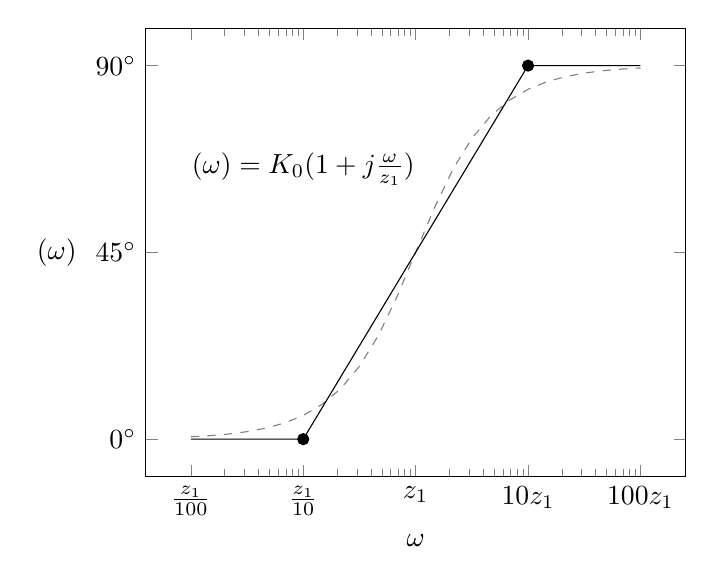
\begin{tikzpicture}
\begin{semilogxaxis}[ytick={0,45,90},yticklabels={$0^{\circ}$,$45^{\circ}$,$90^{\circ}$},xtick={1,10,100,1000,10000},xticklabels={$\frac{z_1}{100}$,$\frac{z_1}{10}$,$z_1$,$10z_1$,$100z_1$},xlabel={$\omega$},ylabel={$\phase{\bH(\omega)}$},ylabel style={rotate=-90}]
\addplot[mark=none,color=gray,dashed,domain=1:10000]{atan(x/100)};
\addplot[mark=none,color=black] coordinates {(1,0) (10,0)  (1000,90) (10000,90)};
\addplot[mark=*,color=black] coordinates {(10,0) };
\addplot[mark=*,color=black] coordinates {(1000,90) };
\addplot[mark=none,color=black] coordinates {(10,65) }node[]{$\bH(\omega)=K_0(1+j\frac{\omega}{z_1})$};
\end{semilogxaxis}
\end{tikzpicture}
\caption{ایک صفر والے تفاعل کا زاویائی بوڈا خط۔}
\label{شکل_تعددی_زاویائی_بوڈا_ایک_صفر_الف}
\end{figure}
%================
\ابتدا{مثال}
تبادلی تفاعل \عددی{\bH(\omega)=\frac{50}{1+j\frac{\omega}{300}}} کا زاویائی بوڈا خط کھینچیں۔

حل:اس تفاعل کا زاویہ ذیل ہے جہاں کونا \عددی{\omega=\SI{300}{\radian\per\second}} پر پایا جاتا ہے۔
\begin{align}
\phase{\bH(\omega)}=\frac{1}{\phase{\tan^{-1} \frac{\omega}{300}}}=\phase{-\tan^{-1}\frac{\omega}{300}}
\end{align}
اس تفاعل کو شکل \حوالہ{شکل_تعددی_زاویائی_بوڈا_ایک_قطب_الف} میں ہلکی سیاہی میں نقطہ دار لکیر سے دکھایا گیا ہے۔

بوڈا خط میں کونے سے دس گنا کم تعدد پر زاویہ \عددی{0^{\circ}} اور کونے سے دس گنا زیادہ تعدد پر زاویہ \عددی{-90^{\circ}} چنتے ہوئے ان نقطوں کو سیدھے خط سے ملایا جاتا ہے۔یوں \عددی{\omega=\SI{30}{\radian\per\second}} پر \عددی{0^{\circ}} اور  \عددی{\omega=\SI{3000}{\radian\per\second}} پر \عددی{90^{\circ}} چنتے ہوئے انہیں سیدھے لکیر سے ملایا گیا ہے۔مزید  \عددی{\omega=\SI{30}{\radian\per\second}} سے کم تعدد پر زاویہ \عددی{0^{\circ}} ہی رکھا جاتا ہے جبکہ \عددی{\omega=\SI{3000}{\radian\per\second}} سے زیادہ تعدد پر زاویہ \عددی{-90^{\circ}} رکھا جاتا ہے۔بوڈا زاویائی خط کو شکل  \حوالہ{شکل_تعددی_زاویائی_بوڈا_ایک_قطب_الف} میں گہری سیاہی میں دکھایا گیا ہے۔
\begin{figure}
\centering
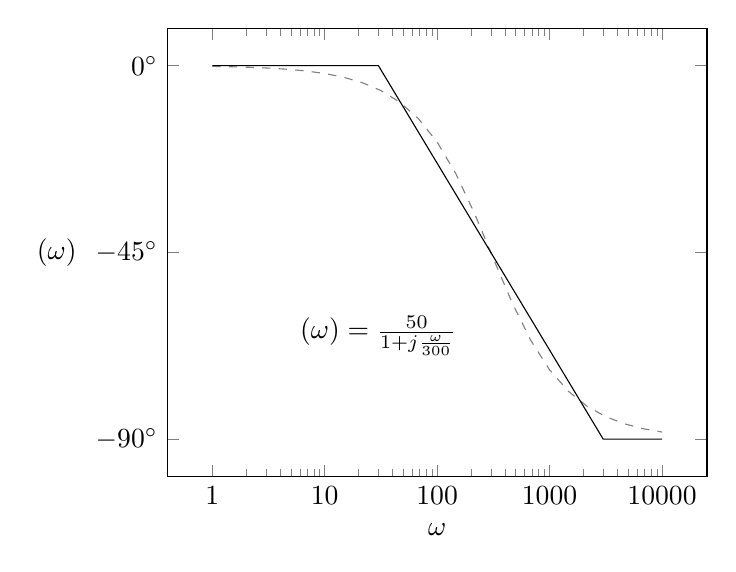
\begin{tikzpicture}
\begin{semilogxaxis}[ytick={0,-45,-90},yticklabels={$0^{\circ}$,$-45^{\circ}$,$-90^{\circ}$},xtick={1,10,100,1000,10000},xticklabels={$1$,$10$,$100$,$1000$,$10000$},xlabel={$\omega$},ylabel={$\phase{\bH(\omega)}$},ylabel style={rotate=-90}]
\addplot[mark=none,color=gray,dashed,domain=1:10000]{-atan(x/300)};
\addplot[mark=none,color=black] coordinates {(1,0) (30,0)  (3000,-90) (10000,-90)};
\addplot[mark=none,color=black] coordinates {(30,-65) }node[]{$\bH(\omega)=\frac{50}{1+j\frac{\omega}{300}}$};
\end{semilogxaxis}
\end{tikzpicture}
\caption{ایک قطب والے تفاعل کا بوڈا زاویائی خط۔}
\label{شکل_تعددی_زاویائی_بوڈا_ایک_قطب_الف}
\end{figure}

یوں کونے \عددی{(\omega=\SI{300}{\radian\per\second})} پر، کونے سے دس گنا زیادہ تعدد \عددی{(\omega=\SI{3000}{\radian\per\second})} پر اور کونے سے دس گنا کم تعدد \عددی{(\omega=\SI{30}{\radian\per\second})} پر زاویے درج ذیل حاصل ہوتے ہیں۔
\begin{align*}
\phase{\bH(200)}&=\phase{-\tan^{-1} \frac{300}{300}}=\phase{-45^{\circ}}\\[0.5ex]
\phase{\bH(2000)}&=\phase{-\tan^{-1} \frac{3000}{300}}=\phase{-84.3^{\circ}}\\[0.5ex]
\phase{\bH(20)}&=\phase{-\tan^{-1} \frac{30}{300}}=\phase{-5.7^{\circ}}
\end{align*}
\انتہا{مثال}
%========================
\ابتدا{مثال}\شناخت{مثال_تعددی_نوے_درجہ_الف}
تبادلی تفاعل \عددی{\bH(\omega)=\frac{j20\omega(1+j\tfrac{\omega}{200})}{1+j\frac{\omega}{\num{30000}}}} کا زاویائی بوڈا خط کھینچیں۔

حل:اس تفاعل کا زاویہ لکھتے ہیں۔
\begin{align*}
\phase{\bH(\omega)}=\phase{90^{\circ}}+\phase{\tan^{-1}\frac{\omega}{200}}-\phase{\tan^{-1}\frac{\omega}{\num{30000}}}
\end{align*}
شمار کنندہ میں \عددی{j20\omega=0+j20\omega} لکھتے ہوئے زاویہ \عددی{\tan^{-1}\tfrac{j20\omega}{0}=90^{\circ}} حاصل ہوتا ہے۔ دوسرا رکن \عددی{\SI{20}{\radian\per\second}} پر \عددی{0^{\circ}} اور \عددی{\SI{2}{\kilo\radian\per\second}} پر \عددی{90^{\circ}} جبکہ تیسرا رکن \عددی{\SI{300}{\radian\per\second}} پر \عددی{0^{\circ}} اور \عددی{\SI{300}{\kilo\radian\per\second}} پر \عددی{-90^{\circ}} ہے۔ان تمام ارکان کو شکل \حوالہ{شکل_تعددی_نوے_درجہ_الف} میں دکھایا گیا ہے۔
\begin{figure}
\centering
\begin{subfigure}{1\textwidth}
\centering
\begin{tikzpicture}
\begin{semilogxaxis}[xlabel={$\omega(\si{\radian\per\second})$},ylabel={$\phase{\bH(\omega)}$},ylabel style={rotate=-90},ytick={-90,-45,0,45,90},yticklabels={$-90^{\circ}$,$-45^{\circ}$,$0^{\circ}$,$45^{\circ}$,$90^{\circ}$}]
\addplot[mark=none,color=black] coordinates {(1,90) (3000000,90)};
\addplot[mark=none,color=black] coordinates {(1,0) (20,0) (2000,90) (3000000,90)};
\addplot[mark=none,color=black] coordinates {(1,0) (3000,0) (30000,-90) (3000000,-90)};
\end{semilogxaxis}
\end{tikzpicture}
\caption*{(الف)}
\end{subfigure}
\begin{subfigure}{1\textwidth}
\centering
\begin{tikzpicture}
\begin{semilogxaxis}[xlabel={$\omega(\si{\radian\per\second})$},ylabel={$\phase{\bH(\omega)}$},ylabel style={rotate=-90},ytick={90,180},yticklabels={$90^{\circ}$,$180^{\circ}$}]
\addplot[mark=none,color=black] coordinates {(1,90) (20,90) (2000,180) (3000,180) (300000,90) (3000000,90)};
\addplot[mark=none,color=gray,dashed,domain=1:3000000]{90+atan(x/200)-atan(x/30000)};
\end{semilogxaxis}
\end{tikzpicture}
\caption*{(ب)}
\end{subfigure}
\caption{مثال \حوالہ{مثال_تعددی_نوے_درجہ_الف} کا زاویائی بوڈا خط۔}
\label{شکل_تعددی_نوے_درجہ_الف}
\end{figure}

\انتہا{مثال}
%=========================
\ابتدا{مثال}
تبادلی تفاعل \عددی{\bH(\omega)=\frac{j10\omega}{(1+j\frac{\omega}{100})(1+j\frac{\omega}{10000})}} کا مقداری بوڈا خط کھینچیں۔

حل:اس تفاعل کی حتمی قیمت 
\begin{align*}
\abs{\bH(\omega)}=\frac{10\omega}{\sqrt{1+\frac{\omega^2}{100^2}}\sqrt{1+\frac{\omega^2}{10000^2}}}
\end{align*}
کو ڈیسی بیل میں لکھتے ہیں۔
\begin{align}\label{مساوات_تعددی_چار_رکنی_بوڈا}
20\log_{10} 10 +20\log_{10}\omega -20\log_{10}\sqrt{1+\frac{\omega^2}{100^2}} -20\log_{10}\sqrt{1+\frac{\omega^2}{10000^2}}
\end{align}
مساوات \حوالہ{مساوات_تعددی_چار_رکنی_بوڈا} کا پہلا رکن \عددی{\SI{20}{\deci\bel}} کا مستقل ہے۔اس کا دوسرا رکن \عددی{\omega=\SI{1}{\radian\per\second}} پر \عددی{\SI{0}{\deci\bel}} کے برابر ہے جبکہ اس تعدد سے زیادہ تعدد پر بتدریج بیس ڈیسی بیل فی دہائی بڑھتا ہے۔تیسرے اور چوتھے ارکان کے بوڈا خط بالترتیب \عددی{\SI{100}{\radian\per\second}}  اور \عددی{\SI{10}{\kilo\radian\per\second}} تعدد پر منفی بیس ڈیسی بیل فی دہائی گھٹنا شروع ہوتے ہیں۔ان تمام ارکان کو شکل \حوالہ{شکل_تعددی_زاویائی_بوڈا_ایک_صفر_دو_قطب_الف}-الف اور ان کا مجموعہ شکل-ب میں دکھایا گیا ہے۔
\begin{figure}
\centering
\begin{subfigure}{1\textwidth}
\centering
\begin{tikzpicture}
\begin{semilogxaxis}[ytick={-40,-20,0,20,40,60},yticklabels={$\SI{-40}{\deci\bel}$,$\SI{-20}{\deci\bel}$,$\SI{0}{\deci\bel}$,$\SI{20}{\deci\bel}$,$\SI{40}{\deci\bel}$,$\SI{60}{\deci\bel}$},xtick={0.1,1,10,100,1000,10000,100000},xticklabels={$10^{-1}$,$10^0$,$10^1$,$10^2$,$10^3$,$10^4$,$10^5$},xlabel={$\omega(\si{\radian\per\second})$},ylabel={$\abs{\bH(\omega)}$}]
%\addplot[mark=none,color=gray,dashed,domain=1:10000]{-atan(x/300)};
\addplot[mark=none,color=black] coordinates {(0.1,20) (100000,20)};
\addplot[mark=none,color=black]coordinates{(0.1,0) (1,0) (100,40)};
\addplot[mark=none,color=black]coordinates{(0.1,0) (100,0) (10000,-40)};
\addplot[mark=none,color=black]coordinates{(0.1,0) (10000,0) (100000,-20)};
\end{semilogxaxis}
\end{tikzpicture}
\caption*{(الف)}
\end{subfigure}
\begin{subfigure}{1\textwidth}
\centering
\begin{tikzpicture}
\begin{semilogxaxis}[ytick={-40,-20,0,20,40,60},yticklabels={$\SI{-40}{\deci\bel}$,$\SI{-20}{\deci\bel}$,$\SI{0}{\deci\bel}$,$+\SI{20}{\deci\bel}$,$+\SI{40}{\deci\bel}$,$+\SI{60}{\deci\bel}$},xtick={0.1,1,10,100,1000,10000,100000},xticklabels={$10^{-1}$,$10^0$,$10^1$,$10^2$,$10^3$,$10^4$,$10^5$},xlabel={$\omega(\si{\radian\per\second})$},ylabel={$\abs{\bH(\omega)}$}]
%\addplot[mark=none,color=gray,dashed,domain=1:10000]{-atan(x/300)};
\addplot[mark=none,color=black] coordinates {(0.1,20) (1,20) (100,60) (10000,60) (100000,40)};
\end{semilogxaxis}
\end{tikzpicture}
\caption*{(ب)}
\end{subfigure}
\caption{ایک صفر اور دو قطب والے تفاعل کا بوڈا مقداری خط۔}
\label{شکل_تعددی_زاویائی_بوڈا_ایک_صفر_دو_قطب_الف}
\end{figure}

ہمیں عموماً درمیانی تعدد پر بوڈا خط میں زیادہ دلچسپی ہوتی ہے۔ایسی صورت میں بوڈا مقداری خط درمیانی تعدد \عددی{(\SI{100}{\radian\per\second} <\omega<\SI{10}{\kilo\radian\per\second})} سے شروع کرنا بہتر ثابت ہوتا ہے۔دونوں کونوں سے دور یعنی \عددی{\omega\ll \SI{10}{\kilo\radian\per\second}} اور \عددی{\omega \gg \SI{100}{\radian\per\second}} پر  \عددی{1+\tfrac{\omega^2}{100^2}\approx \tfrac{\omega^2}{100^2}} اور \عددی{1+\tfrac{\omega^2}{10000^2}=1} لکھتے ہوئے درج ذیل لکھا جا سکتا ہے
\begin{align*}
\abs{\bH(\omega)}=\frac{10\omega}{\left(\sqrt{\frac{\omega^2}{100^2}}\right)\left(\sqrt{1}\right)}=1000 
\end{align*}
لہٰذا درمیانی تعددی پٹی پر ڈیسی بیل میں مقدار درج ذیل ہو گی
\begin{align*}
20\log_{10}\abs{\bH(\omega)}=20\log_{10} 1000=\SI{60}{\deci\bel} 
\end{align*}
 جسے شکل \حوالہ{شکل_تعددی_زاویائی_بوڈا_ایک_صفر_دو_قطب_الف}-ب میں \عددی{\omega=\SI{100}{\radian\per\second}} تا \عددی{\SI{10}{\kilo\radian\per\second}} دکھایا گیا ہے۔چونکہ حقیقت میں پست تعددی کونے  سے کم تعدد پر مقدار مسلسل بیس ڈیسی بیل فی دہائی بڑھتے ہوئے عین \عددی{\omega=\SI{100}{\radian\per\second}}  پر \عددی{\SI{60}{\deci\bel}} تک پہنچتی ہے لہٰذا پست تعددی کونے سے بیس ڈیسی بیل فی دہائی ڈھلوان کا خط کھینچیں۔اسی طرح بلند تعدد کونے پر بھی بیس ڈیسی بیل فی دہائی ڈھلوان کا خط کھینچیں۔یوں مکمل بوڈا خط حاصل ہو گا۔ 
\انتہا{مثال}
%=================
\ابتدا{مثال}\شناخت{مثال_تعددی_چالیس_ڈیسی_بیل_ڈھلوان}
تبادلی تفاعل \عددی{\bH(\omega)=\frac{10\left(1+j\frac{\omega}{10}\right)\left(1+j\frac{\omega}{1000}\right)}{\left(1+j\frac{\omega}{\num{100000}}\right)^2 \left(1+j\frac{\omega}{\num{1000000}}\right)^2}} کا مقداری بوڈا خط کھینچیں۔

حل:تفاول کی مقدار کو ڈیسی بیل میں لکھتے ہیں۔ان کا مجموعہ شکل \حوالہ{شکل_تعددی_چالیس_ڈیسی_بیل_ڈھلوان} میں دکھایا گیا ہے۔
\begin{multline*}
20\log_{10}\abs{\bH(\omega)}=20\log_{10} 10 +20\log_{10} \sqrt{1+\frac{\omega}{10^2}}+20\log_{10}\sqrt{1+\frac{\omega^2}{10^6}} \\
-40\log_{10}\sqrt{1+\frac{\omega^2}{10^10}}-40\log_{10}\sqrt{1+\frac{\omega^2}{10^{12}}}
\end{multline*}
یہاں \عددی{\SI{10}{\radian\per\second}} پر درج بالا مساوات کا دوسرا جزو بیس ڈیسی بیل فی دہائی بڑھنا شروع ہو جات ہے جبکہ تیسرا جزو اسی شرح سے \عددی{\SI{1000}{\radian\per\second}} پر بڑھنا شروع ہوتا ہے۔یوں ان کا مجموعہ لیتے ہوئے \عددی{\SI{1000}{\radian\per\second}} تعدد سے خط کی ڈھلوان \عددی{\SI{40}{\deci\bel}} فی دہائی ہو گی۔اسی طرح \عددی{\SI{100}{\kilo\radian\per\second}} پر چھوتا جزو \عددی{\SI{40}{\deci\bel}} فی دہائی سے گھٹنا شروع ہوتا ہے جو دوسرے اور تیسرے اجزاء کو ختم کرتا ہے لہٰذا بوڈا خط برقرار \عددی{\SI{140}{\deci\bel}} پر رہتا ہے۔آخر کار \عددی{\SI{1}{\mega\radian\per\second}} پر پانچواں جزو چالیس ڈیسی بیل فی دہائی سے گھٹنا شروع ہوتا ہے۔ 
\begin{figure}
\centering
\begin{tikzpicture}
\begin{semilogxaxis}[ytick={0,20,40,60,80,100,120,140,160},yticklabels={$\SI{0}{\deci\bel}$,$\SI{20}{\deci\bel}$,$\SI{40}{\deci\bel}$,$\SI{60}{\deci\bel}$,$\SI{80}{\deci\bel}$,$\SI{100}{\deci\bel}$,$\SI{120}{\deci\bel}$,$\SI{140}{\deci\bel}$,$\SI{160}{\deci\bel}$},xlabel={$\omega(\si{\radian\per\second})$},ylabel={$\abs{\bH(\omega)}$}]
\addplot[mark=none,color=black] coordinates {(1,20) (10,20) (1000,60) (100000,140) (1000000,140) (10000000,100)};
\addplot[mark=none,color=black] coordinates {(200,40)}node[right]{$\SI{20}{\deci\bel}/\text{دہائی}$};
\addplot[mark=none,color=black] coordinates {(3000,80)}node[left]{$\SI{40}{\deci\bel}/\text{دہائی}$};
\addplot[mark=none,color=black] coordinates {(10000000,100)}node[left]{$\SI{-40}{\deci\bel}/\text{دہائی}$};
\end{semilogxaxis}
\end{tikzpicture}
\caption{مثال \حوالہ{مثال_تعددی_چالیس_ڈیسی_بیل_ڈھلوان} کا مقداری بوڈا خط۔}
\label{شکل_تعددی_چالیس_ڈیسی_بیل_ڈھلوان}
\end{figure}

\انتہا{مثال}
%==================

تبادلی تفاعل کے صفر اور قطب مخلوط اعداد بھی ہو سکتے ہیں۔ایسی صورت میں ان کے جوڑی دار جوڑے پائے جاتے ہیں۔آئیں ان پر غور کریں۔تبادلی تفاعل
\begin{align*}
\bH(s)=\frac{K}{(s+a)(s+b)}
\end{align*}
کے قوسین کو ضرب دیتے ہوئے ترتیب دیتے ہیں۔
\begin{align*}
\bH(s)&=\frac{K}{s^2+s(a+b)+ab}\\
&=\frac{K}{ab[1+\frac{s(a+b)}{ab}+\frac{s^2}{ab}]}
\end{align*}
اس کو درج ذیل معیاری صورت میں لکھا جا سکتا ہے
\begin{align}\label{مساوات_تعددی_دو_درجی_قطب}
\bH(s)=\frac{K_0}{1+2\zeta (s \tau)+(s \tau)^2}
\end{align}
جہاں
\begin{align*}
\tau&=\frac{1}{\sqrt{ab}}\\
\zeta&=\frac{a+b}{2\sqrt{ab}}
\end{align*}
کے برابر ہیں۔مساوات \حوالہ{مساوات_تعددی_دو_درجی_قطب} میں \عددی{\zeta}  کو \اصطلاح{تقصیری تناسب}\فرہنگ{تقصیری تناسب}\حاشیہب{damping ration}\فرہنگ{damping ratio} کہتے ہیں۔

فرض کریں کہ ہمیں مساوات \حوالہ{مساوات_تعددی_دو_درجی_قطب} دی گئی ہے اور ہم اس کے قطب جاننا چاہتے ہیں۔قطب جاننے کے لئے نسب نما کے جذر حاصل کرنے ہوں گے جنہیں دو درجی مساوات کے کلیے سے حاصل کیا جا سکتا ہے۔
\begin{align*}
s&=\frac{-2\zeta \tau \mp\sqrt{4\zeta^2\tau^2-4\tau^2}}{2\tau^2}
\end{align*}
جذر کی علامت کے اندر مقدار کی قیمت  صفر سے زیادہ، صفر کے برابر یا صفر سے کم ممکن ہے یعنی
\begin{align*}
4\zeta^2\tau^2-4\tau^2>0\\
4\zeta^2\tau^2-4\tau^2=0\\
4\zeta^2\tau^2-4\tau^2<0
\end{align*}
جن سے  بالترتیب درج ذیل شرائط حاصل ہوتے ہیں۔
\begin{gather}
\begin{aligned}
\zeta&>1 \quad \quad \text{\RL{حقیقی دو عدد مختلف قطب}}\\
\zeta&=1\quad \quad \text{\RL{حقیقی دو عدد یکساں قطب}}\\
\zeta&<1\quad \quad \text{\RL{جوڑی دار مخلوط قطب}}
\end{aligned}
\end{gather}
تقصیری تناسب کی قیمت اکائی سے زیادہ یا اکائی کے برابر ہونے کی صورت میں حقیقی قطب پائے جاتے ہیں جن پر ہم غور کر چکے ہیں۔آئیں مخلوط قطب پر غور کریں۔
%======================
\ابتدا{مشق}
تبادلی تفاعل \عددی{\bH(s)=\frac{35}{4s^2+2s+1}} کا \عددی{\tau} اور \عددی{\zeta} حاصل کریں۔اس تفاعل کے قطب بھی دریافت کریں۔تفاعل کو اجزائے ضربی کی صورت میں لکھیں۔

جواب:\عددی{\tau=2}، \عددی{\zeta=0.5}، \عددی{p_1=-s_1=\tfrac{1}{4}+j\tfrac{\sqrt{3}}{4}}، \عددی{p_2=-s_2=\tfrac{1}{4}-j\tfrac{\sqrt{3}}{4}}،\\
\عددی{\bH(s)=\tfrac{35}{(s+\tfrac{1}{4}+j\tfrac{\sqrt{3}}{4})(s+\tfrac{1}{4}-j\tfrac{\sqrt{3}}{4})}}
\انتہا{مشق}
%=======================

مساوات \حوالہ{مساوات_تعددی_دو_درجی_قطب} میں \عددی{s=j\omega} پر کر کے ترتیب دیتے ہوئے
\begin{align*}
\bH(\omega)&=\frac{K_0}{1+2\zeta (j\omega \tau)+(j\omega \tau)^2}\\
&=\frac{K_0}{1-\omega^2\tau^2 +j 2\zeta\omega \tau}
\end{align*}
اس کی حتمی مقدار کو ڈیسی بیل میں لکھتے ہیں۔
\begin{align}\label{مساوات_تعددی_تقصیری_جزو}
20\log_{10}\abs{\bH(\omega)}=20\log_{10} K_0 -20\log_{10}\sqrt{(1- \omega^2\tau^2)^2+(2\zeta\omega\tau)^2}
\end{align}
مساوات \حوالہ{مساوات_تعددی_تقصیری_جزو} کا پہلا جزو مستقل ہے جبکہ دوسرے جزو کی مقدار کا دارومدار تعدد کے علاوہ تقصیری تناسب پر بھی منحصر  ہے۔ شکل \حوالہ{شکل_تعددی_تقصیری_جزو}-الف میں مختلف \عددی{\zeta} کے  لئے مساوات \حوالہ{مساوات_تعددی_تقصیری_جزو} کے  دوسرے جزو کے خطوط دکھائے گئے ہیں۔اب تک ہم دیکھتے آ رہے ہیں کہ قطب پر مقداری خط گھٹنے شروع ہوتا ہے لیکن یہاں ایسا نہیں ہو رہا ہے۔مخلوط قطبین کی صورت میں مقداری خط گھٹنے سے پہلے بڑھتا ہے۔بڑھنے کی مقدار کا دارومدار \عددی{\zeta} پر ہے۔تقصیری تناسب کی قیمت صفر \عددی{(\zeta=0)} ہو نے کی صورت میں \عددی{\omega \tau=1} پر تفاعل بے قابو بڑھتا ہے۔شکل میں \عددی{\zeta=0.02} کے خط کو نقطہ دار لکیر سے دکھایا گیا ہے۔تقصیری تناسب کی قیمت صفر ہونا دور میں گونج یا \اصطلاح{گمک}\فرہنگ{گمک}\حاشیہب{resonance}\فرہنگ{resonance} کو ظاہر کرتی ہے۔

شکل \حوالہ{شکل_تعددی_تقصیری_جزو}-ب میں تبادلی تفاعل کا زاویائی خط \عددی{\zeta=0.1, 0.2,0.4,0.6,0.8,1} کے لئے دکھایا گیا ہے۔
\begin{figure}
\centering
\begin{subfigure}{1\textwidth}
\centering
\begin{tikzpicture}
\begin{semilogxaxis}[xlabel={$\omega \tau (\si{\radian\per\second})$},ymax=20,ytick={10,0,-10,-20,-30},yticklabels={$\SI{10}{\deci\bel}$,$\SI{0}{\deci\bel}$,$\SI{-10}{\deci\bel}$,$\SI{-20}{\deci\bel}$,$\SI{-30}{\deci\bel}$},xtick={0.1,1,4},xticklabels={$0.1$,$1$,$4$},ylabel style={rotate=-90},ylabel={\RL{مقدار}}]
%
\addplot[mark=none,color=black,dashed,domain=0.1:4,samples=100]{-20*log10(sqrt((1-x^2)^2+(2*0.02*x)^2))}node[pos=0.22,pin={-145:{$\zeta=0.02$}}]{};
\addplot[mark=none,color=black,domain=0.1:4,samples=200]{-20*log10(sqrt((1-x^2)^2+(2*0.1*x)^2))}node[pos=0.25,pin={[inner sep=0pt]30:{$\zeta=0.1$}}]{};
\addplot[mark=none,color=black,domain=0.1:4,samples=100]{-20*log10(sqrt((1-x^2)^2+(2*0.2*x)^2))}node[pos=0.2,pin={[pin distance=1cm]20:{$\zeta=0.2$}}]{};
\addplot[mark=none,color=black,domain=0.1:4,samples=100]{-20*log10(sqrt((1-x^2)^2+(2*0.4*x)^2))}node[pos=0.15,pin={[pin distance=1cm]30:{$\zeta=0.4$}}]{};
\addplot[mark=none,color=black,domain=0.1:4,samples=100]{-20*log10(sqrt((1-x^2)^2+(2*0.6*x)^2))}node[pos=0.25,pin={30:{$\zeta=0.6$}}]{};
\addplot[mark=none,color=black,domain=0.1:4,samples=100]{-20*log10(sqrt((1-x^2)^2+(2*0.8*x)^2))}node[pos=0.18,pin={[outer sep=0pt]-140:{$\zeta=0.8$}}]{};
\addplot[mark=none,color=black,domain=0.1:4,samples=100]{-20*log10(sqrt((1-x^2)^2+(2*1*x)^2))}node[pos=0.6,pin={[inner sep=0pt]-140:{$\zeta=1$}}]{};
\end{semilogxaxis}
\end{tikzpicture}
\caption*{(الف)}
\end{subfigure}
\begin{subfigure}{1\textwidth}
\centering
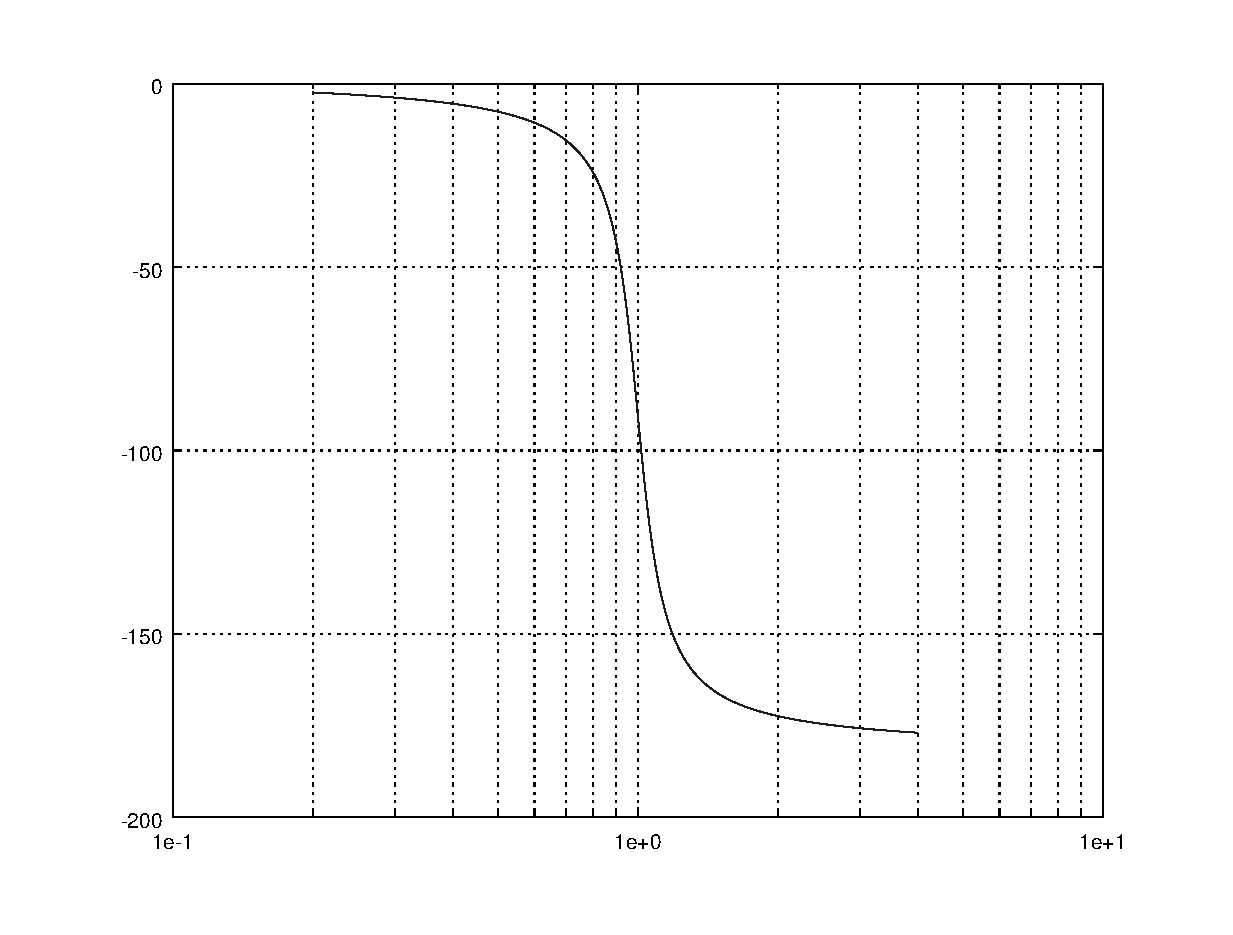
\includegraphics{figFreqDoublePolePhasePlot}
\caption*{(ب)}
\end{subfigure}
\caption{مختلف تقصیری تناسب کے لئے مخلوط جوڑی دار قطب کے تفاعل کے خط۔}
\label{شکل_تعددی_تقصیری_جزو}
\end{figure} 
%=====================

\حصہ{گمکی ادوار}
\حصہء{سلسلہ وار گمک}
شکل \حوالہ{شکل_تعدد_سلسلہ_وار_الف} میں سلسلہ وار دور دکھایا گیا ہے جس کی رکاوٹ
\begin{align}\label{مساوات_سلسلہ_وار_رکاوٹ_الف}
\bZ(\omega)=R+j\omega L +\frac{1}{j\omega C}=R+j(\omega L-\frac{1}{\omega C})
\end{align}
ہے۔قوسین کی قیمت صفر ہونے کی صورت میں اس دور کی رکاوٹ حقیقی مقدار 
\begin{align}
\bZ(\omega)=R
\end{align}
یعنی مزاحمتی ہو گی۔ایسا ایک مخصوص تعدد \عددی{\omega_0} پر ممکن ہے جسے قوسین صفر کے برابر پر کرنے
\begin{align*}
\omega L-\frac{1}{\omega C}=0
\end{align*}
سے حاصل کیا جا سکتا ہے۔
\begin{align}\label{مساوات_تعددی_گمکی_تعدد_سلسلہ_وار}
\omega_0=\frac{1}{\sqrt{LC}}\quad \quad \text{\RL{گمکی تعدد}}
\end{align}
اس تعدد \عددی{(\omega_0)} کو دور کی \اصطلاح{گمکی تعدد}\فرہنگ{گمکی تعدد}\حاشیہب{resonant frequency}\فرہنگ{resonant frequency} کہتے ہیں اور اس تعدد پر دور گونجتا یا گمکتا ہے۔ایسا دور جو گونج سکتا ہو کو \اصطلاح{گمکی دور}\فرہنگ{گمکی دور}\حاشیہب{resonant circuit}\فرہنگ{resonant circuit} کہتے ہیں۔
\begin{figure}
\centering
\begin{tikzpicture}[american voltages]
\draw(0,0) to [short,i={$\hat{I}$}]++(\x/2,0) to [capacitor,l={$C$},v={$\hat{V}_C$}]++(\x,0) to [inductor,l={$L$},v={$\hat{V}_L$}]++(\x,0) to [resistor,l_={$R$},v^<={$\hat{V}_R$}]++(0,-\y) to [short]++(-2*\x-\x/2,0);
\draw(0,0.25) rectangle ++(-0.5,-\y-0.5);
\draw(0,-\y/2)node[right]{$\begin{aligned} &+\\&\hat{V}_d \\ &- \end{aligned}$};
\end{tikzpicture}
\caption{سلسلہ وار \عددی{RLC} دور۔}
\label{شکل_تعدد_سلسلہ_وار_الف}
\end{figure}

گمکی تعدد پر امالی متعاملیت اور برق گیر متعاملیت برابر ہوتے ہیں۔ چونکہ سلسلہ وار دور میں یکساں رو پائی جاتی ہے لہٰذا گمکی تعدد پر امالی دباو اور برق گیر دباو مقدار میں برابر لیکن آپس میں \عددی{180^{\circ}} زاویے پر ہوں گے۔زاویائی طور پر آپس میں بالکل الٹ ہونے کی بنا ان کا مجموعہ صفر کے برابر ہو گا اور یوں شکل \حوالہ{شکل_تعدد_سلسلہ_وار_الف} میں داخلی دباو \عددی{\hat{V}_d} اور مزاحمتی دباو \عددی{\hat{V}_R} برابر ہوں گے۔

گمکی تعدد سے ہٹ کر کسی بھی تعدد پر مساوات \حوالہ{مساوات_سلسلہ_وار_رکاوٹ_الف} کا خیالی جزو صفر کے برابر نہیں ہو گا لہٰذا رکاوٹ کی حتمی قیمت \عددی{R} سے زیادہ ہو گی۔آپ دیکھ سکتے ہیں کہ گمکی تعدد پر رکاوٹ کی قیمت کم سے کم ہو گی اور رو کی قیمت زیادہ سے زیادہ ہو گی۔ گمکی تعدد پر دور میں رو اور داخلی دباو ہم زاویہ ہوں گے۔گمکی تعدد سے کم تعدد پر برق گیر متعاملیت کی مقدار امالی متعاملیت کے مقدار سے زیادہ ہو گی لہٰذا سلسلہ وار رکاوٹ برق گیر خاصیت رکھے گا اور داخلی دباو سے رو آگے پائی جائے گی۔اس کے برعکس گمکی تعدد سے زیادہ تعدد پر امالی متعاملیت کی مقدار برق گیر متعاملیت کی مقدار سے زیادہ ہو گی لہٰذا کل رکاوٹ امالی ہو گا اور داخلی دباو سے رو پیچھے ہو گی۔ رکاوٹ کی مقدار بالمقابل تعدد کو شکل \حوالہ{شکل_تعددی_رکاوٹ_بالمقابل_تعدد_سلسلہ_وار_دور} میں دکھایا گیا ہے۔
\begin{figure}
\centering
\begin{tikzpicture}
\begin{axis}[xlabel={$\omega$},ylabel={$\abs{\bZ(\omega)}$},ylabel style={rotate=-90},xtick={50},xticklabels={${\omega_0=\frac{1}{\sqrt{LC}}}$},ytick={50},yticklabels={$R$}]
\addplot[mark=none,color=black,domain=25:100,samples=100]{sqrt{50^2+(0.02*x-1/(0.02*x))^2}}node[pos=0.05,pin={45:{\RL{برق گیر رکاوٹ}}}]{}node[pos=0.8,pin=125:{\RL{امالی رکاوٹ}}]{};
\addplot[mark=none,color=black] coordinates {(50,50)}node[pin={90:{\RL{مزاحمتی رکاوٹ}}}]{};
\end{axis}
\end{tikzpicture}
\caption{سلسلہ وار \عددی{RLC} کی رکاوٹ بالمقابل تعدد کا خط۔}
\label{شکل_تعددی_رکاوٹ_بالمقابل_تعدد_سلسلہ_وار_دور}
\end{figure}

رو کے حوالے سے تینوں پرزوں کے دباو کے دوری سمتیات شکل \حوالہ{شکل_تعددی_سلسلہ_وار_دوری_سمتیات} میں دکھائے گئے ہیں۔گمکی تعدد سے کم تعدد پر برق گیر کا دباو امالہ گیر کے دباو سے زیادہ ہے لہٰذا داخلی دباو \عددی{\hat{V}_d} سے رو آگے ہے۔گمکی تعدد پر داخلی دباو اور رو ہم زاویہ ہیں جبکہ گمکی تعدد سے زیادہ تعدد پر امالہ کی متعاملیت برق گیر کے متعاملیت سے زیادہ ہے لہٰذا امالی دباو کی قیمت برق گیر دباو سے زیادہ ہے اور یوں داخلی دباو سے رو پیچھے ہے۔داخلی دباو اور رو کے مابین زاویہ \عددی{\theta_z} مساوات \حوالہ{مساوات_سلسلہ_وار_رکاوٹ_الف} میں دیے رکاوٹ کا زاویہ ہے۔
\begin{align}
\theta_z=\tan^{-1}\frac{\omega L-\frac{1}{\omega C}}{R}
\end{align}
%
\begin{figure}
\centering
\begin{tikzpicture}
\pgfmathsetmacro{\l}{2}
\pgfmathsetmacro{\ang}{30}
\pgfmathsetmacro{\kh}{\l*cos(\ang)};
\pgfmathsetmacro{\kv}{\l*sin(\ang)};
%
\draw[-latex](0,0)--++(\x+\x/4,0)node[below]{$\hat{I}$};
\draw[-latex](0,0)--++(\ang:\l)coordinate(kTip)node[above]{$\hat{V}_d$};
\draw[-latex](0,0)--++(\kh,0)node[below]{$\hat{V}_R$};
\draw[-latex](0,0)--++(0,1/2*\y+\kv)node[above]{$\hat{V}_L$};
\draw[-latex](0,0)--++(0,-1/2*\y)node[below]{$\hat{V}_C$};
\draw([shift={(0:0.5)}]0,0) arc (0:\ang:0.5);
\draw(3/4*\ang:0.5)node[right]{$\theta_z$};
\draw[gray,dashed](kTip)--++(-\kh,0);
\draw[gray,dashed](kTip)--++(0,-\kv);
\draw(3/4*\x,-\y)node{$(\omega > \omega_0)$};
%
\begin{scope}[xshift=3cm]
\draw[-latex](0,0)--++(\x+\x/4,0)node[below]{$\hat{I}$};
\draw[-latex](0,0)--++(0:\l)coordinate(kTip)node[above,pos=0.7]{$\hat{V}_R=\hat{V}_d$};
\draw[-latex](0,0)--++(0,3/4*\y)node[above]{$\hat{V}_L$};
\draw[-latex](0,0)--++(0,-3/4*\y)node[below]{$\hat{V}_C$};
\draw(3/4*\x,-\y)node{$(\omega = \omega_0)$};
\end{scope}
%
\begin{scope}[xshift=6cm]
\draw[-latex](0,0)--++(\x+\x/4,0)node[below]{$\hat{I}$};
\draw[-latex](0,0)--++(-\ang:\l)coordinate(kTip)node[below]{$\hat{V}_d$};
\draw[-latex](0,0)--++(\kh,0)node[above]{$\hat{V}_R$};
\draw[-latex](0,0)--++(0,1/2*\y)node[above]{$\hat{V}_L$};
\draw[-latex](0,0)--++(0,-1/2*\y-\kv)node[below]{$\hat{V}_C$};
\draw([shift={(0:0.5)}]0,0) arc (0:-\ang:0.5);
\draw(-3/4*\ang:0.5)node[right]{$\theta_z$};
\draw[gray,dashed](kTip)--++(-\kh,0);
\draw[gray,dashed](kTip)--++(0,\kv);
\draw(3/4*\x,-\y)node{$(\omega <\omega_0)$};
\end{scope}
\end{tikzpicture}
\caption{سلسلہ وار \عددی{RLC} کے دوری سمتیات۔}
\label{شکل_تعددی_سلسلہ_وار_دوری_سمتیات}
\end{figure}

سلسلہ وار \عددی{RLC} دور کا \اصطلاح{معیاری مستقل}\فرہنگ{معیاری مستقل}\حاشیہب{quality factor}\فرہنگ{quality factor} \عددی{Q} نہایت اہم مقدار ہے جس کی تعریف درج ذیل مساوات دیتی ہے۔
\begin{align}\label{مساوات_تعددی_معیاری_مستقل_تعریف}
Q=\frac{\omega_0 L}{R}=\frac{1}{\omega_0 CR}=\frac{1}{R}\sqrt{\frac{L}{C}}
\end{align}
گمکی تعدد پر \عددی{\omega_0 L=\tfrac{1}{\omega_0 C}} ہوتا ہے لہٰذا رکاوٹ
\begin{align*}
\bZ=R+j\left(\omega_0 L-\frac{1}{\omega_0 C}\right)=R
\end{align*}
ہو گا جس سے 
\begin{align*}
\hat{I}=\frac{\hat{V}_d}{\bZ}=\frac{\hat{V}_d}{R}
\end{align*}
اور
\begin{align*}
\hat{V}_L&=j\omega_0 L \hat{I}=\frac{j\omega_0 L \hat{V}_d}{R}\\
\hat{V}_C&=\frac{\hat{I}}{j\omega C}=\frac{\hat{V}_d}{j\omega R C}\\
\hat{V}_R&=\hat{I} R=\hat{V}_d
\end{align*}
حاصل ہوتے ہیں۔درج بالا مساوات میں دونوں جانب حتمی قیمتیں لیتے ہوئے گمکی تعدد کے لئے درج ذیل لکھا جا سکتا ہے
\begin{gather}
\begin{aligned}\label{مساوات_تعددی_گمکی_دباو_تعلقات}
V_L&=Q V_d\\
V_C&=Q V_d\\
V_R&=V_d
\end{aligned}
\end{gather}
 جہاں دباو کے حتمی قیمتوں کو \عددی{V_L}، \عددی{V_C}، \عددی{V_R}  اور \عددی{V_d} لکھا گیا ہے۔مساوات \حوالہ{مساوات_تعددی_گمکی_دباو_تعلقات} کے تحت گمکی تعدد پر امالی دباو اور برق گیر دباو کی قیمتیں داخلی دباو کے \عددی{Q} گنا ہوں گے۔یوں \عددی{Q>1} کی صورت میں امالی اور برق گیر دباو کی قیمت داخلی دباو سے زیادہ ہو گی۔ 
%===============
\ابتدا{مثال}\شناخت{مثال_تعددی_سلسلہ_وار_گمکی_تعدد_الف}
شکل \حوالہ{شکل_تعددی_سلسلہ_وار_گمکی_تعدد_الف} کے دور کی گمکی تعدد اور معیاری مستقل دریافت کریں۔گمکی تعدد پر رو حاصل کرتے ہوئے تینوں پرزوں کے دباو حاصل کریں۔
\begin{figure}
\centering
\begin{tikzpicture}[american voltages]
\draw(0,0) to [short,i={$\hat{I}$}]++(\x/2,0) to [capacitor,l={$\SI{5}{\micro\farad}$},v={$\hat{V}_C$}]++(\x,0) to [inductor,l={$\SI{2}{\milli\henry}$},v={$\hat{V}_L$}]++(\x,0) to [resistor,l_={$\SI{2}{\ohm}$},v^<={$\hat{V}_R$}]++(0,-\y) to [short]++(-2*\x-\x/2,0) to [american voltage source,l={$40\phase{0^{\circ}}\,\si{\volt}$}]++(0,\y);
\end{tikzpicture}
\caption{مثال \حوالہ{مثال_تعددی_سلسلہ_وار_گمکی_تعدد_الف} کا دور۔}
\label{شکل_تعددی_سلسلہ_وار_گمکی_تعدد_الف}
\end{figure}

حل:گمکی تعدد اور معیاری مستقل دریافت کرتے ہیں۔
\begin{align*}
\omega_0&=\frac{1}{\sqrt{LC}}=\frac{1}{\sqrt{2\times 10^{-3}\times 5\times 10^{-6}}}=\SI{10}{\kilo\radian\per\second}\\
Q&=\frac{\omega_0 L}{R}=\frac{\num{10000}\times 2\times 10^{-3}}{2}=10
\end{align*}
گمکی تعدد پر رو حاصل کرتے ہیں۔
\begin{align*}
\hat{I}&=\frac{40\phase{0^{\circ}}}{2+j10000\times 2\times 10^{-3}-\frac{j}{10000\times 5 \times 10^{-6}}}=20\phase{0^{\circ}}\,\si{\ampere}
\end{align*}
چونکہ گمکی تعدد پر رکاوٹ مزاحمتی ہوتا ہے لہٰذا رو کو \عددی{i=\tfrac{40\phase{0^{\circ}}}{2}=20\phase{0^{\circ}}\,\si{\ampere}} سے بھی حاصل کیا جا سکتا ہے۔

پرزوں کے دباو حاصل کرتے ہیں۔
\begin{align*}
\hat{V}_R&=\hat{I} R=(20\phase{0^{\circ}})(2)=40\phase{0^{\circ}}\,\si{\volt}\\
\hat{V}_L&=(j\omega_0 L) \hat{I}=j \num{10000}\times 2\times 10^{-3} \times 20\phase{0^{\circ}}=400\phase{90^{\circ}}\,\si{\volt}\\
\hat{V}_C&=\left(\frac{-j}{\omega_0 C}\right) \hat{I}=\frac{-j\times 20\phase{0^{\circ}}}{\num{10000}\times 5\times 10^{-6}}=400\phase{-90^{\circ}}\,\si{\volt}
\end{align*}
دباو کے یہی جوابات مساوات \حوالہ{مساوات_تعددی_گمکی_دباو_تعلقات} کی مدد سے بھی حاصل کئے جا سکتے ہیں یعنی
\begin{align*}
V_R&=V_d=\SI{40}{\volt}\\
V_L&=Q V_d=10\times 40=\SI{400}{\volt}\\
V_C&=Q V_d=10\times 40=\SI{400}{\volt}
\end{align*}
جہاں مزاحمتی دباو اور داخلی دباو ہم زاویہ ہیں جبکہ امالی دباو اور برق گیر دباو بالترتیب داخلی دباو سے \عددی{90^{\circ}} آگے اور پیچھے ہیں۔ اس مثال میں \عددی{Q=10} ہے لہٰذا گمکی تعدد پر امالی اور برق گیر دباو کی قیمتیں داخلی دباو سے دس گنا زیادہ ہیں۔ 
\انتہا{مثال}
%=================
\ابتدا{مثال}\شناخت{مثال_تعددی_امالہ_معیاری_مستقل}
برق گیر استعمال کرتے ہوئے ضروری ہے کہ برق گیر کی استعداد سے تجاوز نہ کیا جائے۔برق گیر پر اس کے استعداد سے زیادہ دباو ڈالنے سے برق گیر غیر فعال ہو جائے گا۔برق گیر عموماً غیر فعال ہونے کی صورت میں خوفناک دھماکے سے پھٹتا ہے۔ جزو طاقت درست کرنے والے برق گیر یا کارخانوں میں دیگر استعمال ہونے والے بڑے جسامت کے برق گیر کا پھٹنا جان لیوا ثابت ہو سکتا ہے۔

آپ جانتے ہیں کہ تار لپیٹنے سے امالہ گیر بنایا جاتا ہے۔یوں نہ چاہتے ہوئے بھی امالہ گیر میں درکار امالی رکاوٹ کے ساتھ ساتھ غیر مطلوب مزاحمتی رکاوٹ بھی پایا جاتا ہے۔شکل \حوالہ{شکل_تعددی_امالہ_معیاری_مستقل} میں ایسا ہی امالہ گیر اور برق گیر سلسلہ وار جوڑے گئے ہیں جہاں \عددی{L=\SI{90}{\milli\henry}} اور \عددی{C=\SI{100}{\micro\farad}} ہیں۔امالہ گیر کا معیاری مستقل \عددی{Q=6} ہے۔برق گیر پر گمکی تعدد پر دباو حاصل کریں۔
\begin{figure}
\centering
\begin{tikzpicture}
\draw(0,0) to [american voltage source,l={$30\phase{0^{\circ}}\,\si{\volt}\,\rms$}]++(0,\y) to [resistor,l={$R$}]++(\x,0) to [inductor,l={$L$}]++(\x,0) to [capacitor,l={$C$}]++(0,-\y) to [short] (0,0);
\end{tikzpicture}
\caption{مثال \حوالہ{مثال_تعددی_امالہ_معیاری_مستقل} اور مشق \حوالہ{مشق_تعددی_امالہ_معیاری_مستقل_ب} کا دور۔}
\label{شکل_تعددی_امالہ_معیاری_مستقل}
\end{figure}

حل:معیاری مستقل کی قیمت سے گمکی تعدد پر برق گیر کا دباو درج ذیل حاصل ہوتا ہے۔
\begin{align*}
V_C=Q V_d=6\times 30=\SI{180}{\volt}\,\rms
\end{align*}
یوں اس دور کو استعمال کرنے سے پہلے تسلی کر لیں کہ استعمال ہونے والے برق گیر کی استعداد کم از کم \عددی{\SI{180}{\volt}\,\rms} ہے۔
\انتہا{مثال}
%==================
\ابتدا{مشق}\شناخت{مشق_تعددی_امالہ_معیاری_مستقل_ب}
شکل \حوالہ{شکل_تعددی_امالہ_معیاری_مستقل} میں \عددی{C=\SI{10}{\micro\farad}} ہے اور گمکی تعدد پر \عددی{I=\SI{15}{\ampere}\,\rms} اور \عددی{V_C=\SI{120}{\volt}\,\rms} ہیں۔امالہ اور مزاحمت دریافت کریں۔

جوابات:\عددی{R=\SI{2}{\ohm}}، \عددی{L=\SI{0.64}{\milli\henry}}
\انتہا{مشق}
%==================
\ابتدا{مشق}
سلسلہ وار \عددی{RLC} دور میں داخلی دباو \عددی{22\cos \omega t\,\si{\volt}} ہے۔مزاحمت \عددی{\SI{2}{\ohm}} اور \عددی{L=\SI{120}{\micro\henry}} ہے۔دور کی گمکی تعدد \عددی{f_0=\SI{10}{\kilo\hertz}} کے لئے درکار برق گیر معلوم کریں۔دور میں \عددی{f_0}، \عددی{\tfrac{f_0}{2}} اور \عددی{2f_0} پر رو دریافت کریں۔

جوابات:\عددی{C=\SI{2.11}{\micro\farad}}، \عددی{11\cos(20000\pi t)\,\si{\ampere}}، \\
\عددی{1.92\cos(10000\pi+80^{\circ})\,\si{\ampere}}، \عددی{1.92\cos(40000\pi-80^{\circ})\,\si{\ampere}}
\انتہا{مشق}
%=================

آئیں شکل \حوالہ{شکل_تعدد_سلسلہ_وار_الف} میں دکھائے گئے سلسلہ وار \عددی{RLC} دور  میں \عددی{\tfrac{\hat{V}_R}{\hat{V}_d}} تناسب کے لئے \عددی{Q}، \عددی{\omega_0} اور \عددی{\omega} پر مبنی عمومی مساوات حاصل کریں۔مساوات \حوالہ{مساوات_تعددی_معیاری_مستقل_تعریف} سے \عددی{\tfrac{L}{R}=\tfrac{Q}{\omega_0}} اور \عددی{\tfrac{1}{RC}=Q\omega_0} کو دور کے رکاوٹ میں  پر کرتے ہیں۔
\begin{align*}
\bZ(j\omega)&=R+j\big(\omega L-\frac{1}{\omega C}\big)\\
&=R\big[1+j\big(\frac{\omega L}{R} -\frac{1}{\omega RC}\big)\big]\\
&=R\big[1+jQ\big(\frac{\omega}{\omega_0}-\frac{\omega_0}{\omega}\big)\big]
\end{align*}
دور میں رو
\begin{align*}
\hat{I}&=\frac{\hat{V}_d}{Z}\\
&=\frac{\hat{V}_d}{R\big[1+jQ\big(\frac{\omega}{\omega_0}-\frac{\omega_0}{\omega}\big)\big]}
\end{align*}
سے مزاحمتی دباو \عددی{\hat{V}_R=\hat{I} R} لکھ کر دباو کا تناسب لکھتے ہیں
\begin{align*}
\frac{\hat{V}_R}{\hat{V}_d}&=\frac{1}{1+jQ\big(\frac{\omega}{\omega_0}-\frac{\omega_0}{\omega}\big)}
\end{align*}
جس کی حتمی مقدار \عددی{M(\omega)} اور زاویہ \عددی{\phi(\omega)} درج ذیل ہیں جنہیں شکل \حوالہ{شکل_تعددی_مقداری_اور_زاویائی_خط} میں دکھایا گیا ہے۔
\begin{align}
M(\omega)&=\frac{1}{\sqrt{1+Q^2\big(\frac{\omega}{\omega_0}-\frac{\omega_0}{\omega}\big)^2}}\label{مساوات_تعددی_مقداری_عمومی}\\
\phi(\omega)&=-\tan^{-1} Q\big(\frac{\omega}{\omega_0}-\frac{\omega_0}{\omega}\big)\label{مساوات_تعددی_زاویائی_عمومی}
\end{align}
%
\begin{figure}
\centering
\begin{subfigure}{1\textwidth}
\centering
\begin{tikzpicture}
\pgfmathsetmacro{\wL}{-1+sqrt(2)}
\pgfmathsetmacro{\wH}{1+sqrt(2)}
\pgfmathsetmacro{\hp}{1/sqrt(2)}
\pgfmathsetmacro{\kyL}{1/sqrt(1+0.25*(\wL-1/\wL)^2)}
%
\begin{semilogxaxis}[xlabel={$\omega$},ylabel style={rotate=-90},ylabel={$M(\omega)$},xtick={\wL,1,\wH},xticklabels={$\omega_L$,$\omega_0$,$\omega_H$},ytick={\hp,1},yticklabels={$\frac{1}{\sqrt{2}}$,$1$}]
\addplot[mark=none,color=black,domain=0.04:40,samples=40]{1/sqrt(1+0.25*(x-1/x)^2)};
\addplot[mark=none,color=black,dashed,stealth-stealth] coordinates {(\wL,\hp) (\wH,\hp)} node[pos=0.5,fill=white]{$\BW$};
\end{semilogxaxis}
\end{tikzpicture}
\caption*{(الف)}
\end{subfigure}
\begin{subfigure}{1\textwidth}
\centering
\begin{tikzpicture}
\pgfmathsetmacro{\wL}{-1+sqrt(2)}
\pgfmathsetmacro{\wH}{1+sqrt(2)}
\pgfmathsetmacro{\hp}{1/sqrt(2)}
\begin{semilogxaxis}[xlabel={$\omega$},ylabel style={rotate=-90},ylabel={$\phi(\omega)$},xtick={\wL,1,\wH},xticklabels={$\omega_L$,$\omega_0$,$\omega_H$},ytick={90,45,0,-45,-90},yticklabels={${+90^{\circ}}$,${+45^{\circ}}$,${0^{\circ}}$,${-45^{\circ}}$,${-90^{\circ}}$}]
\addplot[mark=none,color=black,domain=0.04:40,samples=100]{-atan(0.5*(x-1/x))};
\end{semilogxaxis}
\end{tikzpicture}
\caption*{(ب)}
\end{subfigure}
\caption{مقدار بالمقابل تعدد اور زاویہ بالمقابل تعدد کے خط۔}
\label{شکل_تعددی_مقداری_اور_زاویائی_خط}
\end{figure}

مقدار بالمقابل تعدد کا خط \اصطلاح{پٹی گزار چھلنی}\فرہنگ{پٹی گزار چھلنی}\حاشیہب{band-pass filter}\فرہنگ{band-pass filter} کی طرح ہے۔آئیں اس کے کونے دریافت کرتے ہیں۔کونوں پر طاقت کی قیمت نصف ہوتی ہے۔نصف طاقت \عددی{\tfrac{1}{\sqrt{2}}} گنا رو پر پایا جاتا ہے یوں مساوات \حوالہ{مساوات_تعددی_مقداری_عمومی} میں \عددی{M(\omega)=\tfrac{1}{\sqrt{2}}} پر کرنے سے کونوں کی تعدد (انقطاعی تعدد) دریافت کئے جا سکتے ہیں۔
\begin{align*}
\frac{1}{\sqrt{1+Q^2\big(\frac{\omega}{\omega_0}-\frac{\omega_0}{\omega}\big)^2}}=\frac{1}{\sqrt{2}}
\end{align*}
اس سے
\begin{align*}
Q\left(\frac{\omega}{\omega_0}-\frac{\omega_0}{\omega}\right)=\mp 1
\end{align*}
یعنی
\begin{align*}
\omega=\mp \frac{\omega_0}{2Q}\mp \omega_0 \sqrt{\frac{1}{(2Q)^2}+1}
\end{align*}
حاصل ہوتا ہے۔منفی تعدد کے جوابات رد کرتے ہوئے صرف مثبت جوابات تسلیم کرتے ہوئے درج ذیل کونے حاصل ہوتے ہیں۔
 \begin{align}
\omega_L &=\omega_0\left[-\frac{1}{2Q}+ \sqrt{\frac{1}{(2Q)^2}+1}\right]\\
\omega_H &=\omega_0\left[+\frac{1}{2Q}+ \sqrt{\frac{1}{(2Q)^2}+1}\right]
\end{align}
پست تعددی کونے \عددی{\omega_L} اور بلند تعددی کونے \عددی{\omega_H}  کے مابین خطہ \اصطلاح{عرض پٹی}\فرہنگ{عرض پٹی}\حاشیہب{bandwidth}\فرہنگ{bandwidth} کہلاتا  اور \عددی{\BW} سے ظاہر کیا جاتا ہے۔ 
\begin{align}\label{مساوات_تعددی_عرض_پٹی_تعریف}
\BW=\omega_H-\omega_L=\frac{\omega_0}{Q} \quad \quad \text{\RL{عرض پٹی}}
\end{align}
عرض پٹی کے مساوات کو درج ذیل بھی لکھا جا سکتا ہے۔
\begin{align}
\BW=\frac{\omega_0}{Q}=\frac{\frac{1}{\sqrt{LC}}}{\frac{1}{R}\sqrt{\frac{L}{C}}}=\frac{R}{L}
\end{align}
چونکہ کونوں پر طاقت گھٹ کر نصف رہ جاتا ہے اور نصف طاقت \عددی{\SI{-3}{\deci\bel}} کہلاتا ہے لہٰذا تعددی پٹی کو \اصطلاح{تین ڈیسی بیل پٹی}\فرہنگ{پٹی!تین ڈیسی بیل}\حاشیہب{\SI{3}{\deci\bel} bandwidth}\فرہنگ{bandwidth!\SI{3}{\deci\bel}} بھی کہتے ہیں۔

کونوں کے تعدد کو ضرب دینے سے درج ذیل حاصل ہوتا ہے لہٰذا گمکی تعدد دونوں انقطاعی تعدد کا ہندسی اوسط ہے۔ 
\begin{align}
\omega_H \omega_L=\omega_0^2
\end{align}
پست انقطاعی کونے پر زاویہ \عددی{45^{\circ}}، بلند انقطاعی کونے پر \عددی{-45^{\circ}} اور گمکی تعدد پر \عددی{0^{\circ}} ہے۔
%=========================
\ابتدا{مشق}
شکل \حوالہ{شکل_تعددی_سلسلہ_وار_گمکی_تعدد_الف} کے دور کی پست انقطاعی تعدد \عددی{\omega_L}، بلند انقطاعی تعدد \عددی{\omega_H} اور عرض پٹی \عددی{\BW} دریافت کریں۔

جوابات:\عددی{\omega_L=\SI{9512}{\radian\per\second}}، \عددی{\omega_H=\SI{10512}{\radian\per\second}}، \عددی{\BW=\SI{1000}{\radian\per\second}}
\انتہا{مشق}
%======================

مساوات \حوالہ{مساوات_تعددی_معیاری_مستقل_تعریف} کے تحت زیادہ \عددی{Q} کے لئے کم \عددی{R} درکار ہے اور مساوات \حوالہ{مساوات_تعددی_عرض_پٹی_تعریف} کے تحت تنگ عرض پٹی کے لئے زیادہ \عددی{Q} درکار ہے۔یوں تنگ \عددی{Q} کم \عددی{R} کی صورت میں حاصل ہو گا۔تنگ عرض پٹی کا دور نہایت عمدگی سی مخصوص تعدد کو چننے کی صلاحیت رکھتا ہے۔شکل \حوالہ{شکل_تعددی_عرض_پٹی_بالمقابل_معیاری_مستقل} میں مختلف \عددی{Q} کے لئے مساوات \حوالہ{مساوات_تعددی_مقداری_عمومی} کو دکھایا گیا ہے۔داخلی اشارات سے صرف وہ اشارات خارجی جانب پہنچتے ہیں جو عرض پٹی پر پائے جاتے ہوں۔عرض پٹی سے باہر تعدد کے اشارات گھٹتے ہیں۔یوں \عددی{RLC} بطور پٹی گزار چھلنی کام کرتا ہے۔
\begin{figure}
\centering
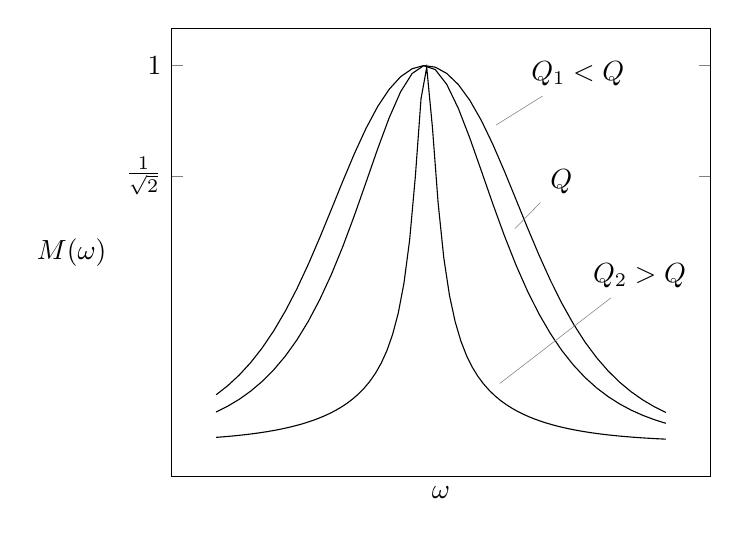
\begin{tikzpicture}
\pgfmathsetmacro{\wL}{-1+sqrt(2)}
\pgfmathsetmacro{\wH}{1+sqrt(2)}
\pgfmathsetmacro{\hp}{1/sqrt(2)}
\pgfmathsetmacro{\kyL}{1/sqrt(1+0.25*(\wL-1/\wL)^2)}
%
\begin{semilogxaxis}[xlabel={$\omega$},ylabel style={rotate=-90},ylabel={$M(\omega)$},xtick=\empty,ytick={\hp,1},yticklabels={$\frac{1}{\sqrt{2}}$,$1$}]
\addplot[mark=none,color=black,domain=0.04:40,samples=40]{1/sqrt(1+0.1*(x-1/x)^2)}node[pos=0.6,pin={45:{$Q_1<Q$}}]{};
\addplot[mark=none,color=black,domain=0.04:40,samples=40]{1/sqrt(1+0.25*(x-1/x)^2)}node[pos=0.65,pin={45:{$Q$}}]{};
\addplot[mark=none,color=black,domain=0.04:40,samples=80]{1/sqrt(1+10*(x-1/x)^2)}node[pos=0.65,pin={[pin distance=1.5cm]45:{$Q_2>Q$}}]{};
\end{semilogxaxis}
\end{tikzpicture}
\caption{عرض پٹی بالمقابل معیاری مستقل۔}
\label{شکل_تعددی_عرض_پٹی_بالمقابل_معیاری_مستقل}
\end{figure}

معیاری مستقل \عددی{Q} کو توانائی کے نقطہ نظر سے دیکھا جا سکتا ہے۔شکل \حوالہ{شکل_تعددی_امالہ_معیاری_مستقل_توانائی_کے_نقطہ_نظر} پر غور کریں جہاں \عددی{RLC} کو گمکی تعدد کا اشارہ مہیا کیا گیا ہے۔گمکی تعدد پر رکاوٹ \عددی{\bZ=R} ہوتی ہے لہٰذا \عددی{i(t)=\tfrac{V_m}{R}\cos \omega_0 t\,\si{\ampere}} اور برق گیر کا دباو 
\begin{align*}
\hat{V}_C=\frac{1}{j\omega_0 C} \hat{I}=\frac{1}{j\omega_0 t}\frac{V_m}{R}\phase{0^{\circ}}=\frac{V_m}{\omega_0 RC}\phase{-90^{\circ}}
\end{align*}
یعنی
\begin{align*}
v_C(t)=\frac{V_m}{\omega_0 RC} \cos (\omega_0 t -90^{\circ})\,\si{\volt}=\frac{V_m}{\omega_0 RC} \sin \omega_0 t \,\si{\volt}
\end{align*}
لکھا جائے گا۔آپ کو یاد ہو گا کہ امالہ گیر میں \عددی{\tfrac{Li^2}{2}} اور برق گیر میں \عددی{\tfrac{Cv^2}{2}} توانائی ذخیرہ ہوتی ہے لہٰذا امالہ گیر کی توانائی
\begin{align}\label{مساوات_تعددی_امالی_ذخیرہ_توانائی}
w_L(t)=\frac{1}{2} L i^2(t)=\frac{1}{2} L \left(\frac{V_m}{R} \cos \omega_0 t\right)^2=\frac{L V_m^2}{2 R^2}\cos^2 \omega_0 t \, \si{\joule}
\end{align}
اور برق گیر کی توانائی
\begin{align*}
w_C(t)=\frac{1}{2} C v^2(t)=\frac{1}{2} C\left(\frac{V_m}{\omega_0 RC} \sin \omega_0 t\right)^2=\frac{V_m^2}{2\omega_0^2 R^2C}\sin^2 \omega_0 t \, \si{\joule}
\end{align*}
لکھی جائے گی۔گمکی تعدد پر \عددی{\omega_0^2=\tfrac{1}{LC}} ہوتا ہے لہٰذا برق گیر کی توانائی کو درج ذیل لکھا جا سکتا ہے۔
\begin{align}\label{مساوات_تعددی_برق_گیر_ذخیرہ_توانائی}
w_C(t)=\frac{V_m^2}{2\frac{1}{LC} R^2C}\sin^2 \omega_0 t=\frac{LV_m^2}{2R^2}\sin^2 \omega_0 t \, \si{\joule}
\end{align}
دور میں کل ذخیرہ توانائی ان دونوں کا مجموعہ ہے
\begin{gather}
\begin{aligned}\label{مساوات_تعددی_کل_ذخیرہ_توانائی}
w_{\text{ذخیرہ}}&=w_L(t)+w_C(t)\\
&=\frac{LV_m^2}{2R^2}\cos^2 \omega_0 t+\frac{LV_m^2}{2R^2}\sin^2 \omega_0 t\\
&=\frac{LV_m^2}{2R^2}
\end{aligned}
\end{gather}
جہاں آخری قدم پر \عددی{\cos^2 \theta+\sin^2 \theta=1} کا استعمال کیا گیا ہے۔یوں دور میں کل ذخیرہ توانائی وقت کے ساتھ تبدیل نہیں ہوتی اور اس کی مقدار اٹل ہے۔
\begin{figure}
\centering
\begin{tikzpicture}[american voltages]
\draw(0,0) to [american voltage source,l={$V_m \cos \omega_0 t\,\si{\volt}$}]++(0,\y) to [resistor,l={$R$},i={$i(t)$}]++(\x,0) to [inductor,l={$L$}]++(\x,0) to [capacitor,l={$C$},v={$v_C(t)$}]++(0,-\y) to [short] (0,0);
\end{tikzpicture}
\caption{سلسلہ وار \عددی{RLC} کو گمکی تعدد کا اشارہ مہیا کیا گیا ہے۔}
\label{شکل_تعددی_امالہ_معیاری_مستقل_توانائی_کے_نقطہ_نظر}
\end{figure}


مساوات \حوالہ{مساوات_تعددی_امالی_ذخیرہ_توانائی} اور مساوات \حوالہ{مساوات_تعددی_برق_گیر_ذخیرہ_توانائی} کو شکل \حوالہ{شکل_تعددی_گمکی_توانائی_تبادلہ} میں دکھایا گیا ہے۔ان مساوات  کے تحت امالہ گیر اور برق گیر میں ذخیرہ توانائی وقت کے ساتھ تبدیل ہوتی ہے جبکہ مساوات \حوالہ{مساوات_تعددی_کل_ذخیرہ_توانائی} کے تحت ان کا مجموعہ اٹل مقدار ہے۔یہ ایک دلچسپ صورت حال ہے۔لمحہ \عددی{\omega_0 t=0^{\circ}} پر امالہ گیر کی توانائی زیادہ سے زیادہ جبکہ برق گیر کی توانائی صفر ہوتی ہے۔اس کے برعکس \عددی{\omega_0 t =90^{\circ}} پر امالہ گیر کی توانائی صفر جبکہ برق گیر کی توانائی زیادہ سے زیادہ ہوتی ہے۔آپ دیکھ سکتے ہیں کہ جیسے جیسے ایک پرزے میں ذخیرہ توانائی گھٹتی ہے ویسے ویسے دوسرے پرزے میں ذخیرہ توانائی بڑھتی ہے۔ہر لمحہ ایک پرزے میں توانائی کی کمی دوسرے پرزے میں توانائی کے اضافے کے برابر ہوتی ہے۔ 

\begin{figure}
\centering
\begin{tikzpicture}
\begin{axis}[xlabel={$\omega_0 t$},ylabel={توانائی},ylabel style={rotate=-90},ytick={0,0.5,1},yticklabels={$0$,$0.5\frac{LV_m^2}{2R^2}$,$\frac{LV_m^2}{2R^2}$},xtick={0,90,180,270,360},xticklabels={$0^{\circ}$,$90^{\circ}$,$180^{\circ}$,$270^{\circ}$,$360^{\circ}$}]
\addplot[mark=none,color=black,domain=0:360,samples=100]{(cos(x))^2}node[pos=0.5,right]{$w_L(t)$};
\addplot[mark=none,color=black,dashed,domain=0:360,samples=100]{(sin(x))^2}node[pos=0.25,right]{$w_C(t)$};
\end{axis}
\end{tikzpicture}
\caption{گمکی دور میں توانائی کا تبادلہ۔}
\label{شکل_تعددی_گمکی_توانائی_تبادلہ}
\end{figure}

گمکی تعدد پر سلسلہ وار \عددی{RLC} میں کل \عددی{\tfrac{LV_m^2}{2R^2}} توانائی ذخیرہ ہوتی ہے۔آئیں تعدد کے ایک چکر میں توانائی کا ضیاع \عددی{w_{\text{ضیاع}}} دریافت کریں۔توانائی صرف مزاحمت میں ضائع ہوتی ہے۔
\begin{align*}
w_{\text{ضیاع}}=\int_0^T i^2(t) R \dif t=\int_0^T \left(\frac{V_m}{R}\cos \omega_0 t\right)^2 R \dif t=\frac{V_m^2 T}{2R}
\end{align*}
کل ذخیرہ توانائی اور فی چکر توانائی کے ضیاع کا تناسب لکھتے ہیں۔
\begin{align*}
\frac{w_{\text{ذخیرہ}}}{w_{\text{ضیاع}}}=\frac{\frac{LV_m^2}{2R^2}}{\frac{V_m^2 T}{2R}}=\frac{L}{RT}=\frac{L}{R \frac{2\pi}{\omega_0}}=\frac{\omega_0 L}{2\pi R}
\end{align*}
چونکہ \عددی{\tfrac{\omega_0 L}{R}=Q} ہے لہٰذا درج ذیل لکھا جا سکتا ہے جو معیاری مستقل \عددی{Q} کی عمومی تعریف  ہے۔
\begin{align}\label{مساوات_تعددی_معیاری_مستقل_عمومی-تعریف}
Q=2\pi \frac{w_{\text{ذخیرہ}}}{w_{\text{ضیاع}}} \quad \quad \text{\RL{معیاری مستقل کی عمومی تعریف}}
\end{align}
معیاری مستقل کی  عمومی تعریف  برقی میدان کے علاوہ میکانی میدان اور سمعی میدان میں بھی استعمال ہوتی ہے۔آپ دیکھ سکتے ہیں کہ کم مزاحمت ضیاع کے دور کا معیاری مستقل زیادہ ہو گا۔ 
%===================
\ابتدا{مثال}
سلسلہ وار \عددی{RLC} دور میں \عددی{R=\SI{1}{\ohm}}، \عددی{L=\SI{2}{\milli\henry}} اور \عددی{C=\SI{20}{\micro\farad}} ہیں۔دور کی \عددی{\omega_0}، \عددی{Q} اور \عددی{\BW} حاصل کریں۔مزاحمت کی قیمت \عددی{R=\SI{0.1}{\ohm}} کرتے ہوئے تینوں قیمتیں دوبارہ حاصل کریں۔

حل:درکار قیمتیں حاصل کرتے ہیں۔
\begin{align*}
\omega_0&=\frac{1}{\sqrt{LC}}=\frac{1}{\sqrt{2\times 10^{-3}\times 20\times 10^{-6}}}=\SI{5000}{\radian\per\second}\\
Q&=\frac{1}{R}\sqrt{\frac{L}{C}}=\frac{1}{1}\sqrt{\frac{2\times 10^{-3}}{20\times 10^{-6}}}=10\\
\BW&=\frac{\omega_0}{Q}=\frac{5000}{10}=\SI{500}{\radian\per\second}
\end{align*}
مزاحمت کی قیمت دس گنا کم کرنے کے بعد تمام قیمتیں دوبارہ حاصل کرتے ہیں۔چونکہ گمکی تعدد میں مزاحمت کا کوئی دخل نہیں ہے لہٰذا اس کی قیمت وہی رہے گی۔
\begin{align*}
Q&=\frac{1}{R}\sqrt{\frac{L}{C}}=\frac{1}{0.1}\sqrt{\frac{2\times 10^{-3}}{20\times 10^{-6}}}=100\\
\BW&=\frac{\omega_0}{Q}=\frac{5000}{100}=\SI{50}{\radian\per\second}
\end{align*}
مزاحمت کی قیمت دس گنا کم کرنے سے معیاری مستقل کی قیمت دس گنا بڑھتی ہے جبکہ عرض پٹی دس گنا کم ہوتی ہے۔
\انتہا{مثال}
%====================
\ابتدا{مشق}
سلسلہ وار \عددی{RLC} دور میں \عددی{R=\SI{2}{\ohm}}، \عددی{L=\SI{1}{\milli\henry}} اور \عددی{C=\SI{2}{\micro\henry}} ہیں۔گمکی تعدد، معیاری مستقل اور عرض پٹی دریافت کریں۔

جوابات:\عددی{\omega_0=\SI{22361}{\radian\per\second}}، \عددی{Q=11.2}، \عددی{\BW=\SI{2000}{\radian\per\second}}
\انتہا{مشق}
%===================
\ابتدا{مشق}
سلسلہ وار \عددی{RLC} دور کا \عددی{R=\SI{5}{\ohm}}، \عددی{\omega_0=\SI{6}{\kilo\radian\per\second}} اور \عددی{\BW=\SI{600}{\radian\per\second}} ہیں۔آپ سے گزارش ہے کہ \عددی{L} اور \عددی{C} دریافت کریں۔

جوابات:\عددی{L=\SI{8.33}{\milli\henry}}، \عددی{C=\SI{3.33}{\micro\farad}}
\انتہا{مشق}
%==================
\ابتدا{مثال}
ایسا سلسلہ وار \عددی{RLC} دور تخلیق دیں کہ \عددی{\omega_0=\SI{1000}{\radian\per\second}} اور \عددی{\BW=\SI{80}{\radian\per\second}} ہوں۔

حل:گمکی تعدد اور عرض پٹی کے مساوات درج ذیل ہیں۔
\begin{align*}
\omega_0&=\frac{1}{\sqrt{LC}}\\
\BW&=\frac{\omega_0}{Q}=\frac{\frac{1}{\sqrt{LC}}}{\frac{1}{R}\sqrt{\frac{L}{C}}}=\frac{R}{L}
\end{align*}
ہم دیکھتے ہیں کہ درکار متغیرات تین جبکہ مساوات دو عدد ہیں۔ تخلیق کے دوران عموماً ایسی ہی مسائل درپیش آتے ہیں جہاں ممکنہ مساوات سے تمام جوابات حاصل کرنا ممکن نہیں ہوتا۔ایسے مسائل تجربے سے حل کئے جاتے ہیں۔تجربے کی بنیاد پر کسی ایک متغیرہ کو چنتے ہوئے بقایا کو مساوات کے ذریعہ حاصل کیا جاتا ہے۔اگر حاصل جوابات قابل قبول نہ ہوں تب متغیرہ کی قیمت تبدیل کرتے ہوئے دوبارہ حل کیا جاتا ہے۔یہ سلسلہ اس وقت تک جاری رکھا جاتا ہے جب تک قابل قبول جوابات حاصل نہ ہوں جائے۔

ہم برق گیر کی قیمت ایسی چنتے ہیں جو دستیاب ہو مثلاً \عددی{C=\SI{10}{\micro\farad}} لہٰذا درج ذیل قیمتیں حاصل ہوتی ہیں۔
\begin{align*}
L&=\frac{1}{\omega_0^2 C}=\frac{1}{1000^2\times 10\times 10^{-6}}=\SI{0.1}{\henry}\\
R&=(L)(\BW)=0.1\times 80=\SI{8}{\ohm}
\end{align*}
\انتہا{مثال}
%===============

مساوات \حوالہ{مساوات_تعددی_گمکی_دباو_تعلقات} کے تحت سلسلہ وار \عددی{RLC} دور میں گمکی تعدد پر امالی دباو اور برق گیر دباو کی قیمتیں داخلی دباو کے \عددی{Q} گنا ہوتی ہیں۔ آئیں دیکھیں کہ آیا امالی دباو اور برق گیر دباو کی زیادہ سے زیادہ قیمت گمکی تعدد پر ہی پائی جاتی ہے یا کہ کسی دوسری تعدد پر۔شکل \حوالہ{شکل_تعددی_برق_گیر_زیادہ_سے_زیادہ-دباو} کو دیکھتے ہوئے برق گیر کا دباو لکھتے ہیں
\begin{align*}
\hat{V}_C&=\left(\frac{\frac{1}{j\omega C}}{R+j\omega L+ \frac{1}{j\omega C}}\right)\hat{V}_m
\end{align*}
جس کو ترتیب دے کر ذیل لکھا جا سکتا ہے۔
\begin{align}\label{مساوات_تعددی_سلسلہ_وار_تبادلی_تفاعل_الف}
\hat{V}_C&=\frac{\hat{V}_m}{1-\omega^2 LC+j\omega RC}
\end{align}
اس کی حتمی قیمت حاصل کرتے  ہیں۔
\begin{align}\label{مساوات_تعدد_زیادہ_دباو_اور_تعدد}
\abs{\hat{V}_C}&=\frac{\abs{\hat{V}_m}}{\sqrt{(1-\omega^2 LC)^2+(\omega RC)^2}}
\end{align}
زیادہ سے زیادہ \عددی{\abs{\hat{V}_C}} پر تعدد \عددی{\omega_{\text{\RL{بلندترطاقت}}}} درج ذیل عمل
\begin{align*}
\frac{\dif \abs{\hat{V}_C}}{\dif \omega}=0
\end{align*}
سے 
\begin{align}
\omega_{\text{\RL{بلندترطاقت}}}=\sqrt{\frac{1}{LC}-\frac{1}{2}\left(\frac{R}{L}\right)^2}
\end{align}
حاصل ہوتی ہے جس میں \عددی{\omega_0^2=\tfrac{1}{LC}} اور \عددی{Q=\tfrac{\omega_0 L}{R}} پر کرتے ہوئے
\begin{gather}
\begin{aligned}\label{مساوات_تعددی_زیادہ_سے_زیادہ_دباو_کی_تعدد}
\omega_{\text{\RL{بلندترطاقت}}}&=\sqrt{\omega_0^2-\frac{1}{2}\left(\frac{\omega_0}{Q}\right)^2}\\
&=\omega_0\sqrt{1-\frac{1}{2Q^2}}
\end{aligned}
\end{gather}
لکھا جا سکتا ہے۔درج بالا مساوات کے تحت زیادہ سے زیادہ دباو گمکی تعدد پر نہیں پایا جاتا اگرچہ \عددی{Q} کی قیمت زیادہ ہونے کی صورت میں درج بالا تعدد تقریباً گمکی تعدد ہی ہو گی۔مساوات \حوالہ{مساوات_تعددی_زیادہ_سے_زیادہ_دباو_کی_تعدد} کو مساوات \حوالہ{مساوات_تعدد_زیادہ_دباو_اور_تعدد} میں پر کرتے ہوئے اور \عددی{\omega_0^2=\tfrac{1}{LC}} اور \عددی{\omega_0^2 R^2 C^2=\tfrac{1}{Q^2}} استعمال کرتے ہوئے زیادہ سے زیادہ دباو کی قیمت حاصل ہوتی ہے
\begin{align}
\abs{\hat{V}_C}_{\text{\RL{بلندتر}}}=\frac{Q\abs{\hat{V}_m}}{\sqrt{1-\frac{1}{4Q^2}}}
\end{align}
جو \عددی{Q\gg1} کی صورت میں درج ذیل قیمت اختیار کرتا ہے۔
\begin{align}
\abs{\hat{V}_C}_{\text{\RL{بلندتر}}}\approx Q\abs{\hat{V}_m}
\end{align}


\begin{figure}
\centering
\begin{tikzpicture}[american voltages]
\draw(0,0) to [american voltage source,l={$\hat{V}_m$}]++(0,\y) to [resistor,l={$R$}]++(\x,0) to [inductor,l={$L$}]++(\x,0) to [capacitor,l={$C$},v={$\hat{V}_C$}]++(0,-\y) to [short] (0,0);
\end{tikzpicture}
\caption{برق گیر پر زیادہ سے زیادہ دباو۔}
\label{شکل_تعددی_برق_گیر_زیادہ_سے_زیادہ-دباو}
\end{figure}
%=======================
\ابتدا{مثال}\شناخت{مثال_تعددی_پسند_اور_معیاری_مستقل}
شکل \حوالہ{شکل_تعددی_برق_گیر_زیادہ_سے_زیادہ-دباو} میں \عددی{L=\SI{10}{\milli\henry}} اور \عددی{C=\SI{1}{\micro\farad}} ہیں۔مزاحمت کی قیمت \عددی{\SI{50}{\ohm}} اور \عددی{\SI{1}{\ohm}} ہونے کی صورت میں  \عددی{\omega_0} اور \عددی{\omega_{\text{\RL{بلندتر}}}} دریافت کریں۔

حل:گمکی تعدد پر مزاحمت کا کوئی اثر نہیں ہے۔
\begin{align*}
\omega_0&=\frac{1}{\sqrt{LC}}=\frac{1}{\sqrt{10\times 10^{-3}\times 1\times 10^{-6}}}=\SI{10}{\kilo\radian\per\second}
\end{align*}
مزاحمت \عددی{\SI{50}{\ohm}} کی صورت میں
\begin{align*}
Q&=\frac{\omega_0 L}{R}=\frac{10000\times 10\times 10^{-3}}{50}=2
\end{align*}
اور
\begin{align*}
\omega_{\text{\RL{بلندتر}}}&=\omega_0\sqrt{1-\frac{1}{2Q^2}}\\
&=10000\sqrt{1-\frac{1}{2\times 2^2}}\\
&=\SI{9354}{\radian\per\second}
\end{align*}
مزاحمت \عددی{\SI{1}{\ohm}} کی صورت میں
\begin{align*}
Q&=\frac{\omega_0 L}{R}=\frac{10000\times 10\times 10^{-3}}{1}=100
\end{align*}
اور
\begin{align*}
\omega_{\text{\RL{بلندتر}}}&=\omega_0\sqrt{1-\frac{1}{2Q^2}}\\
&=10000\sqrt{1-\frac{1}{2\times 100^2}}\\
&\approx \SI{10000}{\radian\per\second}
\end{align*}
حاصل ہوتے ہیں۔

آئیں تبادلی تفاعل \عددی{\tfrac{\hat{V}_C}{\hat{V}_m}} کے خطوط کھینچیں۔مساوات \حوالہ{مساوات_تعددی_سلسلہ_وار_تبادلی_تفاعل_الف} سے  \عددی{R=\SI{50}{\ohm}} کی صورت میں تبادلی تفاعل لکھتے ہیں۔ 
\begin{align}
\frac{\hat{V}_C}{\hat{V}_m}=\frac{1}{1-10^{-8}\omega^2+j50\times 10^{-6}\omega }
\end{align}
اسی طرح \عددی{R=\SI{1}{\ohm}} کی صورت میں تبادلی تفاعل لکھتے ہیں۔
\begin{align}
\frac{\hat{V}_C}{\hat{V}_m}=\frac{1}{1-10^{-8}\omega^2+j1\times 10^{-6}\omega }
\end{align}
ان تبادلی تفاعل کو شکل \حوالہ{شکل_تعددی_پسند_اور_معیاری_مستقل} میں دکھایا گیا ہے۔آپ نے دیکھا کہ زیادہ \عددی{Q} والا جال باریک بینی سے تعدد چنتا ہے جبکہ کم \عددی{Q} والا جال اتنی باریک بینی سے تعدد نہیں چنتا ہے۔
\begin{figure}
\centering
\begin{subfigure}{1\textwidth}
\centering
\includegraphics{figFreqSelevtivityAndQMagnitude}
\caption*{(الف)}
\end{subfigure}
\begin{subfigure}{1\textwidth}
\centering
\includegraphics{figFreqSelevtivityAndQPhase}
\caption*{(ب)}
\end{subfigure}
\caption{مثال \حوالہ{مثال_تعددی_پسند_اور_معیاری_مستقل} کے خطوط۔}
\label{شکل_تعددی_پسند_اور_معیاری_مستقل}
\end{figure}
\انتہا{مثال}
%==========================
\حصہء{متوازی گمک}
اب تک ہم سلسلہ وار \عددی{RLC} کے گمک پر غور کرتے  رہے ہیں۔حقیقت میں متوازی جڑے اور سلسلہ وار جڑے \عددی{RLC} میں مشابہت زیادہ اور فرق کم پایا جاتا ہے۔شکل \حوالہ{شکل_تعددی_متوازی_گمک} میں متوازی \عددی{RLC} دکھایا گیا ہے جس کی کرخوف مساوات رو لکھتے ہیں
\begin{gather}
\begin{aligned}\label{مساوات_تعددی_متوازی_رو_بالمقابل_تعدد}
\hat{I}&=\hat{I}_R+\hat{I}_L+\hat{I}_C\\
&=\frac{\hat{V}_d}{R}+j\omega C \hat{V}_d+\frac{\hat{V}_d}{j\omega L}\\
&=\hat{V}_d\left[G+j\left(\omega C-\frac{1}{\omega L}\right)\right]
\end{aligned}
\end{gather}
جہاں آخری قدم پر \عددی{\tfrac{1}{R}=G} لکھا گیا ہے۔گمکی تعدد \عددی{\omega_0} پر رو کم سے کم ہو گی۔کم سے کم رو \عددی{\omega_0 C=\tfrac{1}{\omega_0 L}} کی حالت میں حاصل ہوتی ہے جس سے گمکی تعدد حاصل ہوتی ہے۔
\begin{align}
\omega_0=\frac{1}{\sqrt{LC}} \quad \quad \text{\RL{گمکی تعدد}}
\end{align}
مساوات \حوالہ{مساوات_تعددی_گمکی_تعدد_سلسلہ_وار} میں سلسلہ وار \عددی{RLC} کی گمکی تعدد دی گئی ہے۔آپ دیکھ سکتے ہیں کہ سلسلہ وار \عددی{RLC} اور متوازی \عددی{RLC} کی گمکی تعدد یکساں ہے۔گمکی تعدد پر رو درج ذیل ہو گی۔
\begin{align}\label{مساوات_تعددی_متوازی_کل_رو}
\hat{I}=G\hat{V}_d
\end{align}
دور کی داخلی فراوانی \عددی{\bY(j\omega)} لکھتے ہیں
\begin{align}
\bY(j\omega)=G+j\omega C+\frac{1}{j\omega L}
\end{align}
جو گمکی تعدد پر درج ذیل ہو گی۔
\begin{align}
\bY(j\omega_0)=R
\end{align}
%
\begin{figure}
\centering
\begin{tikzpicture}
\draw(0,0) to [american voltage source,l={$\hat{V}_d$}]++(0,\y) to [short,i={$\hat{I}$}]++(\x,0) to [short,i={$\hat{I}_X$}]++(\x,0) to [short]++(\x,0) to [inductor,l={$L$},i={$\hat{I}_L$}]++(0,-\y) to [short] (0,0);
\draw(\x,0) to [resistor,*-*,l={$R$},i<_={$\hat{I}_R$}]++(0,\y);
\draw(2*\x,0) to [capacitor,*-*,l={$C$},i<_={$\hat{I}_C$}]++(0,\y);
\end{tikzpicture}
\caption{متوازی \عددی{RLC} کی گمک۔}
\label{شکل_تعددی_متوازی_گمک}
\end{figure}

شکل \حوالہ{شکل_تعددی_متوازی_گمک} میں گمکی تعدد پر امالی اور برق گیر رو کا مجموعہ حاصل کرتے ہیں۔
\begin{align*}
\hat{I}_X&=\hat{I}_C+\hat{I}_L\\
&=j \hat{V}_d\left(\omega_0 C -\frac{1}{\omega_0 L}\right)\\
&=\SI{0}{\ampere}
\end{align*}
اس نتیجے کو سمجھنے کی خاطر  شکل \حوالہ{شکل_تعددی_گمکی_تعدد_متوازی_رکاوٹ} میں دکھائے گئے متوازی جڑے امالہ گیر اور برق گیر کا مجموعی رکاوٹ \عددی{\bZ_0} لکھتے ہیں
\begin{align*}
\frac{1}{\bZ_0}&=j\omega_0 C +\frac{1}{j\omega L}\\
&=j\left(\omega_0 C-\frac{1}{\omega_0 L}\right)\\
&=0
\end{align*}
جس سے  رکاوٹ لامتناہی حاصل ہوتی ہے۔
\begin{align}
\bZ_0=\infty
\end{align}
سلسلہ وار جڑے امالہ گیر اور برق گیر کی گمکی تعدد پر مجموعی رکاوٹ صفر ہوتی ہے جبکہ متوازی جڑے امالہ گیر اور برق گیر کی گمکی تعدد پر رکاوٹ لامتناہی ہوتی ہے۔لامتناہی رکاوٹ میں رو کی قیمت صفر ہی متوقع ہے۔اگرچہ گمکی تعدد پر امالہ گیر اور برق گیر کی مجموعی رو صفر کے برابر ہے، ان کی انفرادی رو ہرگز صفر نہیں ہے۔
\begin{align*}
\hat{I}_C&=j\omega_0 C \hat{V}_d\\
\hat{I}_L&=-j\frac{\hat{V}_d}{\omega_0 L}
\end{align*} 
گمکی تعدد پر امالی رو اور برق گیر رو قیمت میں برابر لیکن زاویائی طور پر آپس میں الٹ قدم \عددی{(180^{\circ})} ہوتی ہیں۔ شکل \حوالہ{شکل_تعددی_متوازی_گمک} میں گمکی تعدد پر رو \عددی{\hat{I}=G\hat{V}_d} ہو گی۔لامتناہی مزاحمت کی صورت میں \عددی{G=\SI{0}{\siemens}} ہو گا لہٰذا ایسی صورت میں \عددی{\hat{I}=\SI{0}{\ampere}} ہو گی جبکہ \عددی{\hat{I}_C} اور \عددی{\hat{I}_L} درج بالا مساوات کے تحت ہوں گی۔یہاں بھی امالہ گیر اور برق گیر کے مابین توانائی کا تبادلہ ہوتا ہے۔جیسے جیسے ایک میں توانائی گھٹتی ہے ویسے ویسے دوسرے میں توانائی کا اضافہ ہوتا ہے۔
%
\begin{figure}
\centering
\begin{tikzpicture}
\draw(0,0) to [short,o-]++(2*\x,0) to [inductor,l_={$j\omega_0 L$}]++(0,\y) to [short,-o]++(-2*\x,0);
\draw(\x,0) to [capacitor,*-*,l_={$\frac{1}{j\omega_0 C}$}]++(0,\y);
\draw[stealth-](\x/4,\y/2)--++(-\x/4,0)--++(0,-\y/8)node[below]{$\bZ_0 = \infty$};
\end{tikzpicture}
\caption{گمکی تعدد پر متوازی جڑے امالہ گیر اور برق گیر کی مجموعی رکاوٹ لامتناہی ہے۔}
\label{شکل_تعددی_گمکی_تعدد_متوازی_رکاوٹ}
\end{figure}

مساوات \حوالہ{مساوات_تعددی_متوازی_رو_بالمقابل_تعدد} سے تبادلی تفاعل \عددی{\tfrac{\hat{I}}{\hat{V}_d}} لکھتے ہیں۔
\begin{align}
\frac{\hat{I}}{\hat{V}_d}=\bY(j\omega)=G+j\left(\omega C-\frac{1}{\omega L}\right)
\end{align}
شکل \حوالہ{شکل_تعددی_فراوانی_بالمقابل_تعدد} میں اس تبادلی تفاعل کا حتمی قیمت بالمقابل تعدد خط دکھایا گیا ہے۔گمکی تعدد پر امالی تاثیر زیادہ غالب ہے جبکہ زیادہ تعدد پر برق گیر تاثیر زیادہ غالب ہے۔عین گمکی تعدد پر ایصالی فراوانی پائی جاتی ہے۔
\begin{figure}
\centering
\begin{tikzpicture}
\begin{semilogxaxis}[xlabel={$\omega$},ylabel style={rotate=-90},ylabel={$\abs{\bY(\omega)}$},ytick={1},yticklabels={$G$},xtick={1},xticklabels={$\omega_0=\frac{1}{\sqrt{LC}}$}]
\addplot[mark=none,color=black,domain=0.1:10,samples=50]{sqrt(1+(x-1/x)^2)}node[pos=0.15,pin=45:{\RL{امالی فراوانی}}]{}node[pos=0.8,pin=125:{\RL{برق گیر فراوانی}}]{};
\addplot[mark=none,color=black] coordinates {(1,1)}node[pin=90:{\RL{ایصالی فراوانی}}]{};
\end{semilogxaxis}
\end{tikzpicture}
\caption{فراوانی کی مقدار بالمقابل تعدد۔}
\label{شکل_تعددی_فراوانی_بالمقابل_تعدد}
\end{figure}
شکل \حوالہ{شکل_تعددی_متوازی_دوری_سمتیات} میں داخلی دباو \عددی{\hat{V}_d} کے حوالے سے متوازی \عددی{RLC} کے دوری سمتیات دکھائے گئے ہیں۔ گمکی تعدد سے کم تعدد پر امالی رو غالب ہے لہٰذا داخلی دباو سے رو پیچھے ہے جبکہ گمکی تعدد سے زیادہ تعدد پر برق گیر رو زیادہ غالب ہے لہٰذا داخلی دباو سے رو آگے ہے۔عین گمکی تعدد پر داخلی دباو اور رو ہم قدم ہیں۔
\begin{figure}
\centering
\begin{tikzpicture}
\pgfmathsetmacro{\l}{2}
\pgfmathsetmacro{\ang}{30}
\pgfmathsetmacro{\kh}{\l*cos(\ang)};
\pgfmathsetmacro{\kv}{\l*sin(\ang)};
%
\draw[-latex](0,0)--++(\x+\x/4,0)node[below]{$\hat{V}_d$};
\draw[-latex](0,0)--++(\ang:\l)coordinate(kTip)node[above]{$\hat{I}$};
\draw[-latex](0,0)--++(\kh,0)node[below]{$\hat{I}_G$};
\draw[-latex](0,0)--++(0,1/2*\y+\kv)node[above]{$\hat{I}_C$};
\draw[-latex](0,0)--++(0,-1/2*\y)node[below]{$\hat{I}_L$};
\draw([shift={(0:0.5)}]0,0) arc (0:\ang:0.5);
\draw(3/4*\ang:0.5)node[right]{$\theta_z$};
\draw[gray,dashed](kTip)--++(-\kh,0);
\draw[gray,dashed](kTip)--++(0,-\kv);
\draw(3/4*\x,-\y)node{$(\omega > \omega_0)$};
%
\begin{scope}[xshift=3cm]
\draw[-latex](0,0)--++(\x+\x/4,0)node[below]{$\hat{V}_d$};
\draw[-latex](0,0)--++(0:\l)coordinate(kTip)node[above,pos=0.7]{$\hat{I}_G=\hat{I}$};
\draw[-latex](0,0)--++(0,3/4*\y)node[above]{$\hat{I}_C$};
\draw[-latex](0,0)--++(0,-3/4*\y)node[below]{$\hat{I}_L$};
\draw(3/4*\x,-\y)node{$(\omega = \omega_0)$};
\end{scope}
%
\begin{scope}[xshift=6cm]
\draw[-latex](0,0)--++(\x+\x/4,0)node[below]{$\hat{V}_d$};
\draw[-latex](0,0)--++(-\ang:\l)coordinate(kTip)node[below]{$\hat{I}$};
\draw[-latex](0,0)--++(\kh,0)node[above]{$\hat{I}_G$};
\draw[-latex](0,0)--++(0,1/2*\y)node[above]{$\hat{I}_C$};
\draw[-latex](0,0)--++(0,-1/2*\y-\kv)node[below]{$\hat{I}_L$};
\draw([shift={(0:0.5)}]0,0) arc (0:-\ang:0.5);
\draw(-3/4*\ang:0.5)node[right]{$\theta_z$};
\draw[gray,dashed](kTip)--++(-\kh,0);
\draw[gray,dashed](kTip)--++(0,\kv);
\draw(3/4*\x,-\y)node{$(\omega <\omega_0)$};
\end{scope}
\end{tikzpicture}
\caption{متوازی \عددی{RLC} کے دوری سمتیات۔}
\label{شکل_تعددی_متوازی_دوری_سمتیات}
\end{figure}

مساوات \حوالہ{مساوات_تعددی_معیاری_مستقل_عمومی-تعریف} میں معیاری مستقل کی عمومی تعریف بیان کی گئی ہے۔آئیں اس کو استعمال کرتے ہوئے متوازی \عددی{RLC} دور کا \عددی{Q} دریافت کریں۔

شکل \حوالہ{شکل_تعددی_متوازی_گمک} میں داخلی دباو گمکی تعدد پر تصور کرتے ہوئے \عددی{\hat{V}_d=V_m\phase{0^{\circ}}\,\si{\volt}} یعنی \عددی{v_d=V_m\cos \omega_0 t \,\si{\volt}} فرض کریں۔امالہ گیر کی رو
\begin{align}\label{مساوات_تعددی_متوازی_رو_الف}
\hat{I}_L=\frac{\hat{V}_d}{j\omega_0 L}=\frac{V_m\phase{0^{\circ}}}{j\omega_0 L}=\frac{V_m}{\omega_0 L}\phase{-90^{\circ}}
\end{align}
یعنی
\begin{align*}
i_L(t)=\frac{V_m}{\omega_0 L} \cos (\omega_0 t -90^{\circ})=\frac{V_m}{\omega_0 L} \sin \omega_0 t \,\si{\ampere}
\end{align*}
لکھی جائے گی۔ برق گیر اور مزاحمت کی رو درج ذیل لکھی جائے گی۔
\begin{gather}
\begin{aligned}\label{مساوات_تعددی_متوازی_رو_ب}
\hat{I}_C&=\omega_0 C V_m \phase{90^{\circ}} \, \si{\ampere}\\
\hat{I}_G&=GV_m\phase{0^{\circ}}\,\si{\ampere}
\end{aligned}
\end{gather}

امالہ گیر میں ذخیرہ توانائی
\begin{align}\label{مساوات_تعددی_متوازی_امالی_ذخیرہ_توانائی}
w_L(t)=\frac{1}{2} L i_L^2(t)=\frac{1}{2} L \left(\frac{V_m}{\omega_0 L} \sin \omega_0 t\right)^2=\frac{V_m^2}{2\omega_0^2 L}\sin^2 \omega_0 t \, \si{\joule}
\end{align}
اور برق گیر میں ذخیرہ توانائی
\begin{align*}
w_C(t)=\frac{1}{2} C v_C^2(t)=\frac{1}{2} C\left(V_m \cos \omega_0 t\right)^2=\frac{CV_m^2}{2}\cos^2 \omega_0 t \, \si{\joule}
\end{align*}
لکھی جائے گی۔گمکی تعدد پر \عددی{\omega_0^2=\tfrac{1}{LC}} ہوتا ہے لہٰذا امالہ گیر کی توانائی کو درج ذیل لکھا جا سکتا ہے۔
\begin{align}\label{مساوات_تعددی_متوازی_امالہ_گیر_ذخیرہ_توانائی}
w_L(t)=\frac{V_m^2}{2\frac{1}{LC} L}\sin^2 \omega_0 t=\frac{CV_m^2}{2}\sin^2 \omega_0 t \, \si{\joule}
\end{align}
دور میں کل ذخیرہ توانائی ان دونوں کا مجموعہ ہے
\begin{gather}
\begin{aligned}\label{مساوات_تعددی_متوازی_کل_ذخیرہ_توانائی}
w_{\text{ذخیرہ}}&=w_C(t)+w_L(t)\\
&=\frac{CV_m^2}{2}\cos^2 \omega_0 t+\frac{CV_m^2}{2}\sin^2 \omega_0 t\\
&=\frac{CV_m^2}{2}
\end{aligned}
\end{gather}
جہاں آخری قدم پر \عددی{\cos^2 \theta+\sin^2 \theta=1} کا استعمال کیا گیا ہے۔یوں دور میں کل ذخیرہ توانائی وقت کے ساتھ تبدیل نہیں ہوتی اور اس کی مقدار اٹل ہے۔

آئیں اب گمکی تعدد کے ایک چکر میں توانائی کا ضیاع دریافت کریں۔امالہ گیر اور برق گیر میں توانائی کا ضیاع ممکن نہیں ہے۔توانائی صرف \عددی{G} یعنی \عددی{R} میں ضائع ہو گی۔مزاحمت پر \عددی{V_m} حیطے کا دباو لاگو ہے جس کی موثر قیمت \عددی{\tfrac{V_m}{\sqrt{2}}} ہے۔یوں مزاحمت میں طاقتی ضیاع درج ذیل ہو گا۔
\begin{align*}
P_G=\frac{\left(\frac{V_m}{\sqrt{2}}\right)^2}{R}=\frac{GV_m^2}{2}
\end{align*}
گمکی تعدد پر ایک چکر کا دورانیہ \عددی{T=\tfrac{2\pi}{\omega_0}} کے برابر ہے جس میں مزاحمتی ضیاع درج ذیل ہو گا۔
\begin{align}
w_{\text{ضیاع}}=T P_G=\frac{2\pi GV_m^2}{2\omega_0}
\end{align}
مساوات \حوالہ{مساوات_تعددی_معیاری_مستقل_عمومی-تعریف} کو استعمال کرتے ہوئے متوازی \عددی{RLC} دور کا معیاری مستقل حاصل کرتے ہیں۔
\begin{align*}
Q&=2\pi \frac{w_{\text{ذخیرہ}}}{w_{\text{ضیاع}}}\\
&=2\pi \frac{\frac{CV_m^2}{2}}{\frac{2\pi GV_m^2}{2\omega_0}}\\
&=\frac{\omega_0 C}{G}
\end{align*}
گمکی تعدد پر \عددی{\omega_0 C=\tfrac{1}{\omega_0 L}} ہوتا ہے لہٰذا  متوازی \عددی{RLC} کے معیاری مستقل کو درج ذیل لکھا جا سکتا ہے۔
\begin{align}
Q=\frac{\omega_0 C}{G}=\frac{1}{\omega_0 L G}
\end{align}
سلسلہ وار \عددی{RLC} کے \عددی{Q} کے ساتھ موازنہ کرنے سے آپ دیکھ سکتے ہیں کہ متوازی \عددی{RLC} کا \عددی{Q} اس کے بالعکس متناسب ہے۔

مساوات \حوالہ{مساوات_تعددی_متوازی_رو_الف} اور مساوات \حوالہ{مساوات_تعددی_متوازی_رو_الف} متوازی پرزوں کی رو دیتے ہیں جبکہ مساوات \حوالہ{مساوات_تعددی_متوازی_کل_رو} منبع کی رو دیتی ہے۔ان نتائج سے درج ذیل لکھا جا سکتا ہے۔
\begin{gather}
\begin{aligned}
I_L&=Q I\\
I_C&=Q I\\
I_G&=I
\end{aligned}
\end{gather}
یوں متوازی \عددی{RLC} دور میں رو کا کردار وہی ہے جو سلسلہ وار \عددی{RLC} میں دباو کا تھا۔متوازی \عددی{RLC} میں \عددی{Q>1} کی صورت میں گمکی تعدد پر امالہ گیر اور برق گیر کو رو منبع کی رو سے زیادہ ہو گی۔ 
%==================
\ابتدا{مثال}
متوازی جڑے \عددی{RLC} میں \عددی{G=\SI{0.01}{\siemens}}، \عددی{L=\SI{1}{\milli\henry}} اور \عددی{C=\SI{10}{\micro\farad}} ہیں۔اس کو گمکی تعدد پر \عددی{\hat{V}_d=22\phase{0^{\circ}}\,\si{\volt}} دباو فراہم کی جاتی ہے۔گمکی تعدد اور پرزوں میں رو دریافت کریں۔ 

حل:گمکی تعدد دریافت کرتے ہیں۔
\begin{align*}
\omega_0=\frac{1}{\sqrt{LC}}=\frac{1}{\sqrt{10^{-3} \times 10\times 10^{-6}}}=\SI{10}{\kilo\radian\per\second}
\end{align*}
یوں پرزوں کی رو درج ذیل ہو گی۔
\begin{align*}
\hat{I}_G&=G\hat{V}_d=0.01\times 22\phase{0^{\circ}}=0.22\phase{0^{\circ}}\,\si{\ampere}\\
\hat{I}_L&=\frac{\hat{V}_d}{j\omega_0 L}=\frac{22\phase{0^{\circ}}}{j 10000 \times 0.001}=2.2\phase{-90^{\circ}}\,\si{\ampere}\\
\hat{I}_C&=j\omega_0 C \hat{V}_d=j 10000\times 10\times 10^{-5} \times 22\phase{0^{\circ}}=2.2\phase{90^{\circ}}\,\si{\ampere}
\end{align*}
منبع کی رو ان تینوں کا مجموعہ ہو گا جو \عددی{\hat{I}_G} کے برابر ہو گا۔
\begin{align*}
\hat{I}&=\hat{I}_G+\hat{I}_L+\hat{I}_C\\
&=0.22\phase{0^{\circ}}\,\si{\ampere}\\
&=\hat{I}_G
\end{align*}
اس مثال میں امالی رو اور برق گیر رو کی قیمتیں منبع کی رو سے دس گنا زیادہ ہیں۔
\انتہا{مثال}
%====================
\ابتدا{مثال}\شناخت{مثال_تعددی_متوازی_عرض_پٹی}
شکل \حوالہ{شکل_تعددی_متوازی_عرض_پٹی} میں متوازی \عددی{RLC} دور دیا گیا ہے۔اس کا تبادلی تفاعل \عددی{\tfrac{\hat{V}}{\hat{I}}} حاصل کرتے ہوئے  نچلا اور بالائی کونا دریافت کریں۔عرض پٹی بھی حاصل کریں۔
\begin{figure}
\centering
\begin{tikzpicture}[american voltages]
\draw(0,0) to [american current source,l={$\hat{I}_d$}]++(0,\y) to [short]++(3*\x,0) to [inductor,l_={$L$},v^<={$\hat{V}_0$}]++(0,-\y) to [short] (0,0);
\draw(\x,0) to [resistor,*-*,l={$R$}]++(0,\y);
\draw(2*\x,0) to [capacitor,*-*,l={$C$}]++(0,\y);
\end{tikzpicture}
\caption{مثال \حوالہ{مثال_تعددی_متوازی_عرض_پٹی} کا دور۔}
\label{شکل_تعددی_متوازی_عرض_پٹی}
\end{figure}

حل:دور کی فراوانی
\begin{align*}
\bY=G+j(\omega C-\frac{1}{\omega L})
\end{align*}
استعمال کرتے ہوئے خارجی دباو لکھتے ہوئے
\begin{align*}
\hat{V}_0&=\frac{\hat{I}_d}{\bY}\\
&=\frac{\hat{I}_d}{G+j(\omega C-\frac{1}{\omega L})}
\end{align*}
تبادلی تفاعل حاصل کرتے ہیں۔
\begin{align}\label{مساوات_تعددی_متوازی_تبادلی_تفاعل_داخلی_رو}
\frac{\hat{V}_0}{\hat{I}_d}=\frac{1}{G+j(\omega C-\frac{1}{\omega L})}
\end{align}
تبادلی تفاعل عین گمکی تعدد پر زیادہ سے زیادہ ہوتا ہے۔یوں گمکی تعدد پر قوسین صفر کے برابر ہو گی جس سے گمکی تعدد لکھی جا سکتی ہے۔
\begin{align}
\omega_0=\frac{1}{\sqrt{LC}}
\end{align}
گمکی تعدد پر مساوات \حوالہ{مساوات_تعددی_متوازی_تبادلی_تفاعل_داخلی_رو} میں قوسین صفر کے برابر ہے لہٰذا اس کو درج ذیل لکھا جا سکتا ہے جو تفاعل کی زیادہ سے زیادہ قیمت ہے۔
\begin{align}\label{مساوات_تعددی_متوازی_تبادلی_تفاعل_زیادہ}
\frac{\hat{V}_0}{\hat{I}_d}=\frac{1}{G}
\end{align}
گمکی تعدد پر تبادلی تفاعل کی مقدار زیادہ سے زیادہ مقدار کی \عددی{\tfrac{1}{\sqrt{2}}} گنا ہو گی۔یوں کونوں پر درج ذیل لکھا جا سکتا ہے۔
\begin{align}
\frac{1}{\sqrt{G^2+(\omega C-\frac{1}{\omega L})^2}}=\left(\frac{1}{G}\right)\left(\frac{1}{\sqrt{2}}\right)
\end{align}
دونوں اطراف کا مربع لیتے اور ترتیب دیتے ہوئے درج ذیل حاصل ہوتا ہے
\begin{align}
\omega^2\mp \omega \frac{G}{C} -\frac{1}{LC}=0
\end{align}
جس کے مثبت تعددی جوابات لکھتے ہیں۔
\begin{align}
\omega_{L}&=-\frac{G}{2C}+\sqrt{\left(\frac{G}{2C}\right)^2+\frac{1}{LC}}\\
\omega_{H}&=+\frac{G}{2C}+\sqrt{\left(\frac{G}{2C}\right)^2+\frac{1}{LC}}
\end{align}
ان کونوں سے عرض پٹی حاصل کرتے ہیں۔
\begin{align}
\BW=\omega_{H}-\omega_{L}=\frac{G}{C}=\frac{1}{RC}
\end{align}
معیاری مستقل حاصل کرتے ہیں۔
\begin{align}
Q=\frac{\omega_0}{\BW}=\frac{1}{G}\sqrt{\frac{C}{L}}=R\sqrt{\frac{C}{L}}
\end{align}
گمکی تعدد ، معیاری مستقل اور عرض پٹی کے مساوات استعمال کرتے ہوئے کونوں کی تعدد کو درج ذیل لکھا جا سکتا ہے۔
\begin{align}
\omega_{L}=\omega_0 \left[-\frac{1}{2Q}+\sqrt{\frac{1}{(2Q)^2}+1}\right]\\
\omega_{H}=\omega_0 \left[+\frac{1}{2Q}+\sqrt{\frac{1}{(2Q)^2}+1}\right]
\end{align}
\انتہا{مثال}
%=====================
\ابتدا{مثال}
متوازی \عددی{RLC} میں \عددی{R=\SI{1}{\kilo\ohm}}، \عددی{L=\SI{1}{\milli\henry}} اور \عددی{C=\SI{20}{\micro\farad}} ہیں۔گمکی تعدد، معیاری مستقل اور عرض پٹی دریافت کریں۔

حل:
\begin{align*}
\omega_0&=\frac{1}{\sqrt{LC}}=\frac{1}{\sqrt{10^{-3}\times 20 \times 10^{-6}}}=\SI{7071}{\radian\per\second}\\
Q&=R\sqrt{\frac{C}{L}}=1000\sqrt{\frac{10^{-3}}{20\times 10^{-6}}}=141\\
\BW&=\frac{1}{RC}=\frac{1}{1000\times 20\times 10^{-6}}=\SI{50}{\radian\per\second}
\end{align*}
\انتہا{مثال}
%======================
\ابتدا{مثال}
\اصطلاح{برقناطیسی امواج}\فرہنگ{برقناطیسی موج}\حاشیہب{electromagnetic waves}\فرہنگ{electromagnetic waves} کو \اصطلاح{اینٹینا}\فرہنگ{اینٹینا}\حاشیہب{antenna}\فرہنگ{antenna} کے ذریعہ خلاء سے حاصل کرتے ہوئے \اصطلاح{ہمسر ایمپلیفائر}\فرہنگ{ہمسر ایمپلیفائر}\حاشیہب{tuned amplifier}\فرہنگ{tuned amplifier} تک پہنچایا جاتا ہے۔ہمسر ایمپلیفائر مخصوص  عرض پٹی کے اشارات کا حیطہ بڑھاتے ہوئے بقایا تعدد کے اشارات کو گھٹاتا ہے۔تعددی طور پر دو قریبی اشارات کو علیحدہ کرنے کے لئے ضروری ہے کہ ہمسر دور کی عرض پٹی اتنی تنگ ہو کہ اس میں سے صرف درکار اشارات گزر سکے۔ بعض اوقات ایک عدد \عددی{RLC} دور سے اشارات کو علیحدہ کرنا ممکن نہیں ہوتا۔ایسی صورت میں متعدد ہمسر ایمپلیفائر کو زنجیری جوڑا جاتا ہے جہاں پہلے ایمپلیفائر کا خارجی اشارہ دوسرے ایمپلیفائر کو بطور داخلی اشارہ مہیا کیا جاتا ہے۔آئیں دیکھیں کہ زنجیری ایمپلیفائر سے کیسے عرض پٹی مزید تنگ کی جاتی ہے۔

شکل \حوالہ{شکل_تعددی_تنگ_عرض_پٹی}-الف میں زنجیری ایمپلیفائر دکھایا گیا ہے۔داخلی اشارہ \عددی{\hat{V}_d} زنجیری ایمپلیفائر کے پہلی کڑی کو مہیا کیا گیا ہے۔پہلی کڑی کا خارجی اشارہ \عددی{\hat{V}_1} ہے جو دوسری کڑی کو بطور داخلی اشارہ مہیا کیا گیا ہے۔اسی طرح دوسری کڑی کا خارجی اشارہ \عددی{\hat{V}_2} تیسری کڑی کو مہیا کیا گیا ہے۔ شکل-ب میں ایک عدد  ہمسر ایمپلیفائر کا مساوی دور دکھایا گیا ہے۔
\begin{figure}
\centering
\begin{subfigure}{1\textwidth}
\centering
\begin{tikzpicture}
\pgfmathsetmacro{\kl}{\x/2*cos(30)}
\pgfmathsetmacro{\kh}{\x*sin(30)}
%
\draw(0,0)coordinate(ka)--++(150:\x/2)--++(0,-\kh)--++(30:\x/2);
\draw(ka)++(-\kl,0) to [short,-o]++(-\x/4,0)node[above]{$\hat{V}_2$};
\draw(ka)++(0,0) to [short,-o]++(\x/4,0)node[above]{$\hat{V}_3$};
\draw(ka)++(-\kl/2,\kh)node[above]{\RL{تیسری کڑی}};
%
\draw(-\x/2-\kl,0)coordinate(ka)--++(150:\x/2)--++(0,-\kh)--++(30:\x/2);
\draw(ka)++(-\kl,0) to [short,-o]++(-\x/4,0)node[above]{$\hat{V}_1$};
\draw(ka)++(0,0) to [short,-o]++(\x/4,0);
\draw(ka)++(-\kl/2,\kh)node[above]{\RL{دوسری کڑی}};
%
\draw(-\x-2*\kl,0)coordinate(ka)--++(150:\x/2)--++(0,-\kh)--++(30:\x/2);
\draw(ka)++(-\kl,0) to [short,-o]++(-\x/4,0)node[above]{$\hat{V}_d$};
\draw(ka)++(0,0) to [short,-o]++(\x/4,0);
\draw(ka)++(-\kl/2,\kh)node[above]{\RL{پہلی کڑی}};
\end{tikzpicture}
\caption*{(الف) تین درجی زنجیری ایمپلیفائر۔}
\end{subfigure}
\begin{subfigure}{1\textwidth}
\centering
\begin{tikzpicture}
\draw(0,0) to [american controlled current source,l={$A_g \hat{V}_d$}]++(0,-\y)to [short,-o]++(4*\x,0);
\draw(0,0) to [short,-o]++(4*\x,0);
\draw(1.5*\x,-\y) to [resistor,*-*,l={$R$}]++(0,\y);
\draw(2.5*\x,-\y) to [inductor,*-*,l={$L$}]++(0,\y);
\draw(3.5*\x,-\y) to [capacitor,*-*,l={$C$}]++(0,\y);
%
\draw(-\x/2,0) to [short,o-o]++(-\x/2,0);
\draw(0,-\y) to [short,*-o]++(-\x,0);
\draw(-\x,-\y/2)node{$\begin{aligned} &+ \\ &\hat{V}_d \\ &- \end{aligned}$};
\draw(4*\x,-\y/2)node{$\begin{aligned} &+ \\ &\hat{V}_1 \\ &- \end{aligned}$};
\end{tikzpicture}
\caption*{(ب) زنجیری ایمپلیفائر کی ایک کڑی۔}
\end{subfigure}
\caption{زنجیری ہمسر ایمپلیفائر سے عرض پٹی تنگ کی جاتی ہے۔}
\label{شکل_تعددی_تنگ_عرض_پٹی}
\end{figure} 
ہمسر ایمپلیفائر کے دور میں \عددی{\hat{I}_d=-A_g\hat{V}_1} لینے سے شکل \حوالہ{شکل_تعددی_متوازی_عرض_پٹی} حاصل ہوتا ہے لہٰذا مساوات \حوالہ{مساوات_تعددی_متوازی_تبادلی_تفاعل_داخلی_رو} سے پہلے ہمسر ایمپلیفائر کے لئے
\begin{align}\label{مساوات_تعددی_پہلا_ایمپلیفائر}
\hat{V}_1=\frac{-A_g \hat{V}_d}{G+j(\omega C-\frac{1}{\omega L})}
\end{align}
لکھا جا سکتا ہے۔پہلے ایمپلیفائر کا خارجی اشارہ \عددی{\hat{V}_1} ہے جسے دوسرے ایمپلیفائر کو فراہم کیا جاتا ہے لہٰذا مساوات \حوالہ{مساوات_تعددی_متوازی_تبادلی_تفاعل_داخلی_رو} کو دوبارہ استعمال کرتے ہوئے دوسری کڑی کے لئے درج ذیل لکھا جا سکتا ہے
\begin{align*}
\hat{V}_2=\frac{-A_g \hat{V}_1}{G+j(\omega C-\frac{1}{\omega L})}
\end{align*}
جس میں مساوات \حوالہ{مساوات_تعددی_پہلا_ایمپلیفائر} سے \عددی{\hat{V}_1} پر کرتے ہوئے درج ذیل ملتا ہے۔
\begin{align}\label{مساوات_تعددی_دوسرا_ایمپلیفائر}
\hat{V}_2=\frac{(-A_g)^2 \hat{V}_d}{\left[G+j(\omega C-\frac{1}{\omega L})\right]^2}
\end{align}
اسی طرح تیسری کڑی کے لئے درج ذیل لکھ سکتے ہیں۔
\begin{align}\label{مساوات_تعددی_تیسرا_ایمپلیفائر}
\hat{V}_3=\frac{(-A_g)^3 \hat{V}_d}{\left[G+j(\omega C-\frac{1}{\omega L})\right]^3}
\end{align}
ہمسر دور میں \عددی{A_g=\SI{5}{\milli\siemens}}، \عددی{R=\SI{200}{\ohm}}، \عددی{L=\SI{2.2}{\micro\henry}} اور \عددی{C=\SI{5}{\pico\farad}} لیتے ہوئے مساوات \حوالہ{مساوات_تعددی_پہلا_ایمپلیفائر}، مساوات \حوالہ{مساوات_تعددی_دوسرا_ایمپلیفائر} اور مساوات \حوالہ{مساوات_تعددی_تیسرا_ایمپلیفائر} کے مقداری خط شکل \حوالہ{شکل_تعددی_زنجیری_تنگ_پٹی} میں کھینچے گئے ہیں۔آپ دیکھ سکتے ہیں کہ زیادہ تعداد میں ہمسر ایمپلیفائر زنجیری جوڑنے سے عرض پٹی کم ہوتی ہے۔اس مثال میں تمام ہمسر ایمپلیفائر کی گمکی تعدد پر افزائش دباو اکائی \عددی{\bA_v=\SI{1}{\volt\per\volt}} ہے۔
\begin{figure}
\centering
\includegraphics{figFreqTunedAmplifier}
\caption{زنجیری ایمپلیفائر سے عرض پٹی تنگ کرنے کا عمل۔}
\label{شکل_تعددی_زنجیری_تنگ_پٹی}
\end{figure}
یہاں رک کر تسلی کر لیں کہ شکل \حوالہ{شکل_تعددی_تنگ_عرض_پٹی} میں ایمپلیفائر کو استعمال کئے بغیر تین عدد متوازی \عددی{RLC} ادوار کو زنجیری جوڑنے سے  مساوات \حوالہ{مساوات_تعددی_تیسرا_ایمپلیفائر} نہیں ملتی۔بغیر ایمپلیفائر کے تین مزاحمت متوازی جڑ جاتے ہیں جن کا مجموعہ \عددی{\tfrac{R}{3}} ہو گا۔اسی طرح تین امالہ گیر متوازی جوڑنے سے \عددی{\tfrac{L}{3}} ملتا ہے اور تین برق گیر متوازی جوڑنے سے \عددی{3C} ملتا ہے۔یوں صرف \عددی{RLC} زنجیری جوڑنے سے ایک عدد \عددی{RLC} ملتا ہے۔
\انتہا{مثال}
%======================
\ابتدا{مشق}
متوازی \عددی{RLC} میں \عددی{\SI{1}{\kilo\ohm}}، \عددی{L=\SI{0.5}{\milli\henry}} اور \عددی{C=\SI{10}{\micro\farad}} ہیں۔گمکی تعدد، معیاری مستقل اور عرض پٹی دریافت کریں۔

جوابات:\عددی{\omega_0=\SI{14.142}{\kilo\radian\per\second}}، \عددی{Q=141.42}، \عددی{\BW=\SI{100}{\radian\per\second}}
\انتہا{مشق}
%======================
\ابتدا{مشق}
متوازی \عددی{RLC} میں \عددی{R=\SI{4}{\kilo\ohm}}، \عددی{\BW=\SI{2}{\kilo\radian\per\second}} اور \عددی{Q=80} ہیں۔گمکی تعدد \عددی{\omega_0}، امالہ اور برق گیر دریافت کریں۔

جوابات:\عددی{\omega_0=\SI{160}{\kilo\radian\per\second}}، \عددی{L=\SI{0.31}{\milli\henry}}، \عددی{C=\SI{0.125}{\micro\farad}}
\انتہا{مشق}
%=====================

عموماً امالہ گیر کی اندرونی مزاحمت کو نظر انداز نہیں کیا جا سکتا۔ متوازی جڑے امالہ گیر اور برق گیر کا بہتر مساوی دور شکل \حوالہ{شکل_تعددی_بہتر_متوازی_دور} میں دکھایا گیا ہے جس کی داخلی فراوانی درج ذیل ہے۔
\begin{align*}
\bY(j\omega)&=j\omega C+\frac{1}{R+j\omega L}\\
&=j\omega C+\frac{R-j\omega L}{R^2+\omega^2 L^2}\\
&=\frac{R}{R^2+\omega^2 L^2}+j\left(\omega C-\frac{\omega L}{R^2+\omega^2 L^2}\right)
\end{align*}
گمکی تعدد \عددی{\omega'_0} پر فراوانی حقیقی مقدار ہو گی اور خیالی جزو صفر کے برابر ہو گا یعنی
\begin{align}
\omega'_0 C-\frac{\omega'_0 L}{R^2+\omega_0^2 L^2}=0
\end{align}
جس سے گمکی تعدد حاصل ہوتی ہے۔
\begin{align}
\omega'_0=\sqrt{\frac{1}{LC}-\frac{R^2}{L^2}}
\end{align}
%
\begin{figure}
\centering
\begin{tikzpicture}
\draw(0,0) to [short]++(2*\x,0) to [resistor,l_={$R$}]++(0,\y) to [inductor,l_={$L$}]++(0,\y) to [short]++(-2*\x,0);
\draw(\x,0) to [capacitor,*-*,l_={$C$}]++(0,2*\y);
\draw(0,-0.25) rectangle ++(-0.5,2*\y+0.5);
\draw(0,\y) node[right]{$\begin{aligned} &+ \\ \\ \\ &\hat{V}_d \\ \\ \\ &- \end{aligned}$};
\end{tikzpicture}
\caption{متوازی \عددی{LC} کا بہتر مساوی دور۔}
\label{شکل_تعددی_بہتر_متوازی_دور}
\end{figure}
%===================
\ابتدا{مثال}
شکل \حوالہ{شکل_تعددی_بہتر_متوازی_دور} میں \عددی{L=\SI{5}{\milli\henry}} اور \عددی{C=\SI{2.2}{\micro\farad}} ہیں۔تعدد \عددی{\omega_0} اور \عددی{\omega'_0} کو \عددی{R=\SI{20}{\ohm}} اور \عددی{R=\SI{0.5}{\ohm}} کے لئے حاصل کریں۔

حل:دی گئی معلومات سے
\begin{align*}
\omega_0&=\frac{1}{\sqrt{LC}}\\
&=\frac{1}{\sqrt{5\times 10^{-3} \times 2.2 \times 10^{-6}}}\\
&=\SI{9535.6}{\radian\per\second}
\end{align*}
حاصل ہوتا ہے۔مزاحمت \عددی{R=\SI{20}{\ohm}} کے لئے
\begin{align*}
\omega'_0&=\sqrt{\frac{1}{LC}-\frac{R^2}{L^2}}\\
&=\sqrt{\frac{1}{5\times 10^{-3}\times 2.2 \times 10^{-6}} -\left(\frac{20}{5\times 10^{-3}}\right)^2}\\
&=\SI{8655}{\radian\per\second}
\end{align*}
اور مزاحمت \عددی{R=\SI{0.5}{\ohm}} کے لئے
\begin{align*}
\omega'_0&=\sqrt{\frac{1}{LC}-\frac{R^2}{L^2}}\\
&=\sqrt{\frac{1}{5\times 10^{-3}\times 2.2 \times 10^{-6}} -\left(\frac{0.5}{5\times 10^{-3}}\right)^2}\\
&=\SI{9534.1}{\radian\per\second}
\end{align*}
حاصل ہوتے ہیں۔

آپ دیکھ سکتے ہیں کہ کم مزاحمت پر \عددی{\omega'_0} اور \عددی{\omega_0} تقریباً برابر ہوتے ہیں۔
\انتہا{مثال}
%=======================

آئیں گمکی دور کی معلومات کو بوڈا خط کے ساتھ جوڑیں۔ سلسلہ وار \عددی{RLC} کی فراوانی درج ذیل ہے۔
\begin{gather}
\begin{aligned}\label{مساوات_تعددی_فراوانی_سلسلہ_وار}
\bY(j\omega)&=\frac{1}{R+j\left(\omega L-\frac{1}{\omega C}\right)}\\
&=\frac{j\omega C}{(j\omega)^2 LC+j\omega RC+1}
\end{aligned}
\end{gather}
مساوات \حوالہ{مساوات_تعددی_دو_درجی_قطب} کا نسب نما بوڈا خط کا دو درجی جزو دیا گیا ہے
\begin{align*}
(j\omega \tau)^2+2\zeta (j\omega \tau)+1
\end{align*}
جہاں \عددی{\tau=\tfrac{1}{\omega_0}} کے برابر ہے لہٰذا دو درجی جزو کو درج ذیل لکھا جا سکتا ہے۔
\begin{align}\label{مساوات_تعددی_بوڈا_اور_فراوانی}
\frac{(j\omega)^2}{\omega_0^2}+j\frac{2\zeta \omega}{\omega_0}+1
\end{align} 
مساوات \حوالہ{مساوات_تعددی_بوڈا_اور_فراوانی} کا مساوات \حوالہ{مساوات_تعددی_فراوانی_سلسلہ_وار} کے نسب نما سے موازنہ کرتے  ہوئے  درج ذیل لکھا جا سکتا ہے۔
\begin{align*}
\omega_0^2&=\frac{1}{LC}\\
\frac{2\zeta}{\omega_0}&=RC\\
\zeta&=\frac{R}{2}\sqrt{\frac{C}{L}}
\end{align*}
مساوات \حوالہ{مساوات_تعددی_معیاری_مستقل_تعریف} سلسلہ وار \عددی{RLC} کا \عددی{Q} دیتی ہے
\begin{align}
Q=\frac{1}{R}\sqrt{\frac{L}{C}}
\end{align}
لہٰذا درج ذیل لکھا جا سکتا ہے۔
\begin{align}
Q=\frac{1}{2\zeta}
\end{align}
مساوات \حوالہ{مساوات_تعددی_فراوانی_سلسلہ_وار} کا صفر \عددی{\omega=0} پر پایا جاتا ہے لہٰذا اس کے بوڈا خط کی ابتدائی ڈھلوان مثبت بیس ڈیسی بیل فی دہائی ہے۔اب \عددی{Q} کی مقدار درج بالا مساوات کے ذریعہ \عددی{\zeta} سے بندھی ہے لہٰذا زیادہ \عددی{\zeta} کی صورت میں \عددی{Q} کی قیمت کم ہو گی جبکہ کم \عددی{\zeta} کی صورت میں \عددی{Q} کی قیمت زیادہ ہو گی۔شکل \حوالہ{شکل_تعددی_عرض_پٹی_بالمقابل_معیاری_مستقل} میں \عددی{Q} بالمقابل تعدد دکھایا گیا ہے جہاں آپ دیکھ سکتے ہیں کہ  زیادہ \عددی{Q} کی صورت میں عرض پٹی تنگ ہو جاتی ہے۔یہی اثر بوڈا خط میں \عددی{\omega_0} پر بطور چوٹی نظر آتا ہے۔ 

%==========================

\حصہ{چھلنی}
اشارات کو تعدد کی بنیاد پر علیحدہ کرنے کے لئے \اصطلاح{چھلنی}\فرہنگ{چھلنی}\حاشیہب{filter}\فرہنگ{filter} استعمال کی جاتی ہے۔ان میں پست گزار، بلند گزار، پٹی گزار اور پٹی روک چھلنی نہایت مقبول ہیں جن کے خط شکل \حوالہ{شکل_تعددی_چھلنی_کے_اقسام} میں دکھائے گئے ہیں۔\اصطلاح{پست گزار چھلنی}\فرہنگ{پست گزار چھلنی}\فرہنگ{چھلنی!پست گزار}\حاشیہب{low-pass filter}\فرہنگ{low-pass filter}\فرہنگ{filter!low-pass} کسی مخصوص تعدد \عددی{\omega_0} سے کم تعدد کے اشارات کو گزرنے دیتی ہے جبکہ بقایا تعدد کے اشارات کو روکتی ہے۔\اصطلاح{بلند گزار چھلنی}\فرہنگ{بلند گزار چھلنی}\فرہنگ{چھلنی!بلند گزار}\حاشیہب{high-pass filter}\فرہنگ{high-pass filter}\فرہنگ{filter!high-pass} کسی مخصوص تعدد \عددی{\omega_0} سے زیادہ تعدد کے اشارات کو گزرنے دیتی ہے جبکہ بقایا تعدد کے اشارات کو روکتی ہے۔\اصطلاح{پٹی گزار چھلنی}\فرہنگ{پٹی گزار چھلنی}\فرہنگ{چھلنی!پٹی گزار}\حاشیہب{band-pass filter}\فرہنگ{band-pass filter}\فرہنگ{filter!band-pass} کسی مخصوص تعددی پٹی \عددی{\omega_L} تا \عددی{\omega_H} کے اشارات کو گزرنے دیتی ہے جبکہ بقایا تعدد کے اشارات کو روکتی ہے۔\اصطلاح{پٹی روک چھلنی}\فرہنگ{پٹی روک چھلنی}\فرہنگ{چھلنی!پٹی روک}\حاشیہب{band-stop filter}\فرہنگ{band-stop filter}\فرہنگ{filter!band-stop} کسی مخصوص تعددی پٹی \عددی{\omega_L} تا \عددی{\omega_H} کے اشارات کو روکتی ہے جبکہ بقایا تعدد کے اشارات کو گزرنے دیتی ہے۔
\begin{figure}
\centering
\begin{tikzpicture}
\draw(0,0)--++(1.5*\x,0)node[below]{$\omega$};
\draw(0,0)--++(0,\y)node[left]{$\bA_v$};
\draw(0,1)node[left]{$1$}--++(3/4*\x,0)--++(0,-1);
\draw(3/4*\x,0)node[below]{$\omega_0$};
\draw(\x,1.5)node[above]{\RL{کامل پست گزار چھلنی}};
%
\begin{scope}[xshift=-5cm]
\draw(0,0)--++(1.5*\x,0)node[below]{$\omega$};
\draw(0,0)--++(0,\y)node[left]{$\bA_v$};
\draw(0,1)node[left]{$1$};
\draw(3/4*\x,0)--++(0,1)--++(3/4*\x,0);
\draw(3/4*\x,0)node[below]{$\omega_0$};
\draw(\x,1.5)node[above]{\RL{کامل بلند گزار چھلنی}};
\end{scope}
%==================
\begin{scope}[yshift=-5cm]
\draw(0,0)--++(1.5*\x,0)node[below]{$\omega$};
\draw(0,0)--++(0,\y)node[left]{$\bA_v$};
\draw(0,1)node[left]{$1$};
\draw(\x/2,0)node[below]{$\omega_L$}--++(0,1)--++(1,0)--++(0,-1)node[below]{$\omega_H$};
\draw(\x,1.5)node[above]{\RL{کامل پٹی گزار چھلنی}};
\end{scope}
%
\begin{scope}[xshift=-5cm,yshift=-5cm]
\draw(0,0)--++(1.5*\x,0)node[below]{$\omega$};
\draw(0,0)--++(0,\y)node[left]{$\bA_v$};
\draw(0,1)node[left]{$1$};
\draw(0,1)--++(\x/2,0)--++(0,-1)node[below]{$\omega_L$}++(1,0)node[below]{$\omega_H$}--++(0,1)--++(1,0);
\draw(\x,1.5)node[above]{\RL{کامل پٹی روک چھلنی}};
\end{scope}
\end{tikzpicture}
\caption{کامل چھلنیوں کے خط۔}
\label{شکل_تعددی_چھلنی_کے_اقسام}
\end{figure}
%
\begin{figure}
\centering
\begin{subfigure}{0.33\textwidth}
\centering
\begin{tikzpicture}[american voltages]
\draw(0,0) to [american voltage source,l={$\hat{V}_d$}]++(0,\y) to [resistor,l={$R$}]++(\x,0) to [capacitor,l_={$C$},v^<={$\hat{V}_0$}]++(0,-\y) to [short] (0,0);
\end{tikzpicture}
\caption*{(الف) پست گزار چھلنی کا سادہ ترین دور۔}
\end{subfigure}%
\begin{subfigure}{0.66\textwidth}
\centering
\begin{tikzpicture}
\begin{semilogxaxis}[small,xlabel={$\omega$},ylabel={$\abs{\bA_v(j\omega)}$},ylabel style={rotate=-90},ytick={1,0.707},yticklabels={$\SI{0}{\deci\bel}$,$\SI{-3}{\deci\bel}$},xtick={0.1,1,10},xticklabels={$\frac{\omega_0}{10}$,$\omega_0$,$10\omega_0$}]
\addplot[mark=none,color=black] coordinates {(0.1,1)  (1,1) (1,0) (10,0)};
\addplot[mark=none,color=black,domain=0.1:10,samples=30]{1/sqrt(1+x^2)}node[pos=0.6,pin=45:{\RL{حقیقی}}]{};
\addplot[mark=none,color=black]coordinates{(1,0.3)}node[pin=125:{\RL{کامل}}]{};
\end{semilogxaxis}
\end{tikzpicture}
\caption*{(ب) کامل اور حقیقی پست گزار چھلنی کے خط۔}
\end{subfigure}
\caption{پست گزار چھلنی۔}
\label{شکل_تعدد_کامل_پست_گزار_خصلت}
\end{figure}

شکل \حوالہ{شکل_تعدد_کامل_پست_گزار_خصلت}-الف میں پست گزار چھلنی کا سادہ ترین دور دکھایا گیا ہے جس کی افزائش دباو \عددی{\bA_v=\tfrac{\hat{V}_0}{\hat{V}_d}}  درج ذیل ہے
\begin{align*}
\bA_v(j\omega)&=\frac{1}{1+j\omega RC}\\
&=\frac{1}{1+j\omega \tau}
\end{align*} 
جہاں \عددی{RC=\tau} \اصطلاح{وقتی مستقل}\فرہنگ{وقتی مستقل}\حاشیہب{time constant}\فرہنگ{time constant} کہلاتا ہے۔افزائش دباو کی \اصطلاح{مقداری خصلت}\فرہنگ{مقداری خصلت}\فرہنگ{خصلت!مقداری}\حاشیہب{magnitude characteristic}\فرہنگ{magnitude characteristic}  اور \اصطلاح{زاویائی خصلت}\فرہنگ{زاویائی خصلت}\حاشیہب{phase characteristic}\فرہنگ{phase characteristic} لکھتے ہیں۔
\begin{align*}
\abs{\bA_v(\omega)}&=\frac{1}{\sqrt{1+\omega^2 \tau^2}}\\
\phase{\bA_v(\omega)}&=-\tan^{-1} \omega \tau
\end{align*}
شکل \حوالہ{شکل_تعدد_کامل_پست_گزار_خصلت}-ب میں کامل پست گزار چھلنی اور شکل-الف کے حقیقی چھلنی کے خط دکھائے گئے ہیں۔ اگرچہ ہم چاہتے ہیں کہ پست گزار چھلنی کسی مخصوص تعدد \عددی{\omega_0} سے کم تعدد کو جوں کا توں گزارے اور اس سے بلند تعدد کو قطعاً نہیں گزارے، حقیقی ادوار ایسا کرنے سے قاصر ہوتے ہیں۔کامل پست گزار چھلنی \اصطلاح{انقطاعی تعدد}\فرہنگ{انقطاعی تعدد}\حاشیہب{cut-off frequency}\فرہنگ{cut-off frequency} \عددی{\omega_0} سے کم تعدد کو مکمل طور پر گزارتی ہے جبکہ اس سے زیادہ تعدد کو مکمل طور پر روکتی ہے۔حقیقی پست گزار چھلنی بھی یہی کچھ کرتی ہے البتہ انقطاعی تعدد کے قریبی تعدد پر اس کی کارکردگی کامل نہیں ہوتی۔جیسا شکل-ب میں دکھایا گیا ہے، انقطاعی تعدد \عددی{\omega_0} پر حقیقی پست گزار چھلنی کی افزائش دباو \عددی{\A_v} تین ڈیسی بیل کم ہوتی ہے۔جیسا آپ نے بوڈا خطوط میں پڑھا تھا، انقطاعی تعدد کی تعریف یہ ہے کہ اس پر اشارے کی طاقت نصف ہو جائے۔اشارے کا حیطہ \عددی{\tfrac{1}{\sqrt{2}}} گنا ہونے سے اس کی طاقت آدھی ہوتی ہے۔جیسا شکل-ب سے واضح ہے، انقطاعی تعدد سے دور تعدد پر حقیقی پست گزار چھلنی کی کارکردگی یقیناً قابل تعریف ہے۔انقطاعی تعدد سے دس گنا کم \عددی{\tfrac{\omega_0}{10}} یا دس گنا زیادہ \عددی{10\omega_0} تعدد پر اس کی کارکردگی تقریباً کامل چھلنی جیسے ہے۔

شکل \حوالہ{شکل_تعدد_کامل_پست_گزار_خصلت}-الف میں دئے پست گزار چھلنی کو اس طرح سمجھا جا سکتا ہے کہ کم تعدد پر برق گیر کی رکاوٹ زیادہ ہوتی ہے لہٰذا تقسیم دباو کے کلیے سے ظاہر ہے کہ برق گیر پر زیادہ دباو پایا جائے گا۔اس کے برعکس زیادہ تعدد پر برق گیر کی رکاوٹ کم ہوتی ہے لہٰذا تقسیم دباو کے کلیے کے تحت اس پر دباو گھٹ جائے گا۔انتہائی بلند تعدد پر برق گیر کی رکاوٹ انتہائی کم ہو گی اور اس پر دباو قابل نظر انداز ہو گا۔

شکل \حوالہ{شکل_تعدد_کامل_بلند_گزار_خصلت}-الف میں بلند گزار چھلنی کا سادہ ترین دور دکھایا گیا ہے جس کی تبادلی تفاعل لکھتے ہیں جہاں \عددی{RC=\tau} لکھا گیا ہے۔
\begin{align*}
\bA_v(j\omega)&=\frac{R}{R+\frac{1}{j\omega C}}\\
&=\frac{j\omega C}{1+j\omega RC}\\
&=\frac{j\omega \tau}{1+j\omega \tau}
\end{align*}
تبادلی تفاعل کی مقداری اور زاویائی تفاعل لکھتے ہیں۔
\begin{align}
\abs{\bA_v(\omega)}&=\frac{\omega \tau}{\sqrt{1+\omega^2 \tau^2}}\\
\phase{\bA_v(\omega)}=90^{-circ}-\tan^{-1}\omega \tau
\end{align}
شکل-ب میں تبادلی تفاعل کا مقداری خط دکھایا گیا ہے۔ساتھ ہی کامل بلند گزار چھلنی کا خط بھی دکھایا گیا ہے۔یہاں بھی حقیقی چھلنی کی افزائش دباو انقطاعی تعدد پر اشارے کی طاقت آدھی کرتی ہے۔


شکل \حوالہ{شکل_تعدد_کامل_بلند_گزار_خصلت}-الف میں دئے بلند گزار چھلنی کو اس طرح سمجھا جا سکتا ہے کہ صفر تعدد کے قریب برق گیر کی رکاوٹ انتہائی زیادہ ہو گی لہٰذا تقسیم دباو کے کلیے سے ظاہر ہے کہ مزاحمت پر  دباو انتہائی کم ہو گا۔اس کے برعکس انتہائی زیادہ  تعدد پر برق گیر کی رکاوٹ انتہائی کم ہو گی لہٰذا تقسیم دباو کے کلیے کے تحت پورا دباو مزاحمت پر پایا جائے گا۔

\begin{figure}
\centering
\begin{subfigure}{0.33\textwidth}
\centering
\begin{tikzpicture}[american voltages]
\draw(0,0) to [american voltage source,l={$\hat{V}_d$}]++(0,\y) to [capacitor,l={$C$}]++(\x,0) to [resistor,l_={$R$},v^<={$\hat{V}_0$}]++(0,-\y) to [short] (0,0);
\end{tikzpicture}
\caption*{(الف) بلند گزار چھلنی کا سادہ ترین دور۔}
\end{subfigure}%
\begin{subfigure}{0.66\textwidth}
\centering
\begin{tikzpicture}
\begin{semilogxaxis}[small,xlabel={$\omega$},ylabel={$\abs{\bA_v(j\omega)}$},ylabel style={rotate=-90},ytick={1,0.707},yticklabels={$\SI{0}{\deci\bel}$,$\SI{-3}{\deci\bel}$},xtick={0.1,1,10},xticklabels={$\frac{\omega_0}{10}$,$\omega_0$,$10\omega_0$}]
\addplot[mark=none,color=black] coordinates {(0.1,0) (1,0)  (1,1)  (10,1)};
\addplot[mark=none,color=black,domain=0.1:10,samples=30]{x/sqrt(1+x^2)}node[pos=0.2,pin=125:{\RL{حقیقی}}]{};
\addplot[mark=none,color=black]coordinates{(1,0.3)}node[pin=45:{\RL{کامل}}]{};
\end{semilogxaxis}
\end{tikzpicture}
\caption*{(ب) کامل اور حقیقی بلند گزار چھلنی کے خط۔}
\end{subfigure}
\caption{بلند گزار چھلنی۔}
\label{شکل_تعدد_کامل_بلند_گزار_خصلت}
\end{figure}

پٹی گزار چھلنی کا سادہ ترین دور شکل \حوالہ{شکل_تعدد_کامل_پٹی_گزار_خصلت} میں دکھایا گیا ہے۔اس کی افزائش دباو لکھتے ہوئے
\begin{gather}
\begin{aligned}\label{مساوات_تعددی_پٹی_گزار_دور_مساوات}
\bA_v(j\omega)&=\frac{R}{R+j\left(\omega L-\frac{1}{\omega C}\right)}\\
&=\frac{\omega RC}{\omega RC +j(\omega^2 LC-1)}
\end{aligned}
\end{gather}
مقداری تفاعل لکھتے ہیں
\begin{align}\label{مساوات_تعددی_پٹی_گزار_دور_حتمی}
\abs{\bA_v(\omega)}&=\frac{\omega RC}{\sqrt{(\omega RC)^2+(\omega^2 LC-1)^2}}
\end{align}
جس کو شکل-ب میں دکھایا گیا ہے۔اس کی کارکردگی یوں سمجھی جا سکتی ہے کہ درمیانی تعدد یعنی گمکی تعدد \عددی{\omega_0} پر \عددی{\omega L-\tfrac{1}{\omega C}=0} ہوتا ہے لہٰذا داخلی اشارہ جوں کا توں مزاحمت پر پہنچتا ہے۔گمکی تعدد سے بہت کم تعدد پر برق گیر کی رکاوٹ بہت بڑھ جاتی ہے  لہٰذا تقسیم دباو کے کلیے سے ظاہر ہے کہ مزاحمت پر دباو بہت کم ہو گی۔اسی طرح گمکی تعدد سے بہت زیادہ تعدد پر امالی رکاوٹ کی قیمت بہت بڑھ جاتی ہے جس کی وجہ سے مزاحمت پر دباو بہت کم ہوتی ہے۔
%
\begin{figure}
\centering
\begin{subfigure}{0.33\textwidth}
\centering
\begin{tikzpicture}[american voltages]
\draw(0,0) to [american voltage source,l={$\hat{V}_d$}]++(0,\y) to [inductor,l={$L$}]++(\x,0) to [capacitor,l={$C$}]++(\x,0) to [resistor,l_={$R$},v^<={$\hat{V}_0$}]++(0,-\y) to [short] (0,0);
\end{tikzpicture}
\caption*{(الف) پٹی گزار چھلنی کا سادہ ترین دور۔}
\end{subfigure}%
\begin{subfigure}{0.66\textwidth}
\centering
\begin{tikzpicture}
\begin{semilogxaxis}[small,xlabel={$\omega$},ylabel={$\abs{\bA_v(j\omega)}$},ylabel style={rotate=-90},ytick={1,0.707},yticklabels={$\SI{0}{\deci\bel}$,$\SI{-3}{\deci\bel}$},xtick={0.1,1,10,0.618,1.618},xticklabels={$\frac{\omega_0}{10}$,$\omega_0$,$10\omega_0$,$\omega_L$,$\omega_H$}]
\addplot[mark=none,color=black] coordinates {(0.1,0) (0.618,0)  (0.618,1) (1.618,1) (1.618,0) (10,0)};
\addplot[mark=none,color=black,domain=0.1:10,samples=100]{x/sqrt(x^2+(x^2-1)^2)};
\end{semilogxaxis}
\end{tikzpicture}
\caption*{(ب) کامل اور حقیقی پٹی گزار چھلنی کے خط۔}
\end{subfigure}
\caption{پٹی گزار چھلنی۔}
\label{شکل_تعدد_کامل_پٹی_گزار_خصلت}
\end{figure}

مساوات \حوالہ{مساوات_تعددی_پٹی_گزار_دور_مساوات} میں صرف \عددی{\omega} متغیر مقدار ہے۔افزائش دباو کی زیادہ سے زیادہ قیمت  اس تعدد \عددی{\omega_0} پر حاصل ہو گی جس پر نسب نما میں قوسین کی قیمت صفر کے برابر ہو یعنی
\begin{align}
\omega_0=\frac{1}{\sqrt{LC}}
\end{align} 
اس تعدد پر \عددی{\abs{\bA_v(\omega_0)}=\SI{1}{\volt\per\volt}} حاصل ہوتا ہے۔انقطاعی تعدد پر افزائش دباو \عددی{\abs{\bA_v(\omega_0)}} کے \عددی{\tfrac{1}{\sqrt{2}}} گنا ہو گی۔یوں مساوات \حوالہ{مساوات_تعددی_پٹی_گزار_دور_حتمی} کو استعمال کرتے ہوئے انقطاعی تعدد کے لئے درج ذیل لکھا جا سکتا ہے۔
\begin{align*}
\frac{\omega RC}{\sqrt{(\omega RC)^2+(\omega^2 LC-1)^2}}=\frac{1}{\sqrt{2}}
\end{align*}
دونوں جانب مربع لیتے اور ترتیب دیتے ہوئے درج ذیل
\begin{align*}
(\omega^2 LC-1)^2=(\omega RC)^2
\end{align*}
یعنی
\begin{align*}
\omega^2 LC-1=\mp \omega RC
\end{align*}
یا
\begin{align*}
\omega^2 LC\pm \omega RC-1=0
\end{align*}
ملتا ہے۔اس دو درجی مساوات کے حل لکھتے ہیں
\begin{align}
\omega_L&=\frac{-\frac{R}{L}+\sqrt{\left(\frac{R}{L}\right)^2+\frac{1}{LC}}}{2}\\
\omega_H&=\frac{+\frac{R}{L}+\sqrt{\left(\frac{R}{L}\right)^2+\frac{1}{LC}}}{2}
\end{align}
جن سے پٹی گزار چھلنی کی عرض پٹی \عددی{\BW} حاصل ہوتی ہے۔
\begin{align}
\BW=\omega_H-\omega_L=\frac{R}{L}
\end{align}
%===================
\ابتدا{مثال}
اگر آپ کو حساس اشارات کے ساتھ کام کرنا پڑے تو آپ دیکھیں گے کہ ان میں واپڈا کا \عددی{\SI{50}{\hertz}} پایا جاتا ہے جس سے چھٹکارا حاصل کرنا نہایت مشکل ہوتا ہے۔موبائل ٹیلیفون کے زمانے سے پہلے زمینی تار والے ٹیلیفون استعمال کئے جاتے تھے جن کی تاروں میں عموماً \عددی{\SI{50}{\hertz}} کا غیر مطلوب اشارہ گھس جاتا تھا جو شہد کی مکھی کی طرح ہوں ہوں کرتا سنائی دیتا تھا۔

میری بیٹی عفت بریخنہ نے انجنیئرنگ کے آخری سال میں \اصطلاح{برقی قلب نگار}\فرہنگ{برقی قلب نگار}\حاشیہب{electrocardiogram, ecg}\فرہنگ{electrocardiogram}\فرہنگ{ecg} بنایا۔انہیں مسلسل \عددی{\SI{50}{\hertz}} کے غیر مطلوب اشارے کا سامنہ کرنا پڑا۔پچاس ہرٹز کے غیر مطلوب اشارے کی خاصیت یہ ہے کہ اس کی تعدد اٹل ہے۔اس سے \اصطلاح{دندانہ چھلنی}\فرہنگ{دندانہ چھلنی}\فرہنگ{چھلنی!دندانہ}\حاشیہب{notch filter}\فرہنگ{notch filter}\فرہنگ{filter!notch} کی مدد سے چھٹکارا حاصل کیا جاتا ہے۔شکل میں دندانہ چھلنی کا دور دکھایا گیا ہے۔تار کے ٹیلیفون میں \عددی{R} سپیکر کی مزاحمت ہو گی۔برقی قلب نگار میں \عددی{R} اگلے دور کا داخلی تھونن مزاحمت ہو گا۔
\begin{figure}
\centering
\begin{tikzpicture}
\draw(0,0) to [short,o-]++(\x/2,0) to [capacitor,l={$C$}]++(\x,0) to [short,-o]++(\x,0);
\draw(0,-\y) to [short,o-o]++(2*\x+\x/2,0);
\draw(2*\x,0) to [resistor,*-*,l_={$R$}]++(0,-\y);
\draw(\x/2,0) to [short,*-]++(0,-\y/2)to[inductor,l_={$L$}] ++(\x,0) to [short,-*]++(0,\y/2);
\draw(0,-\y/2)node{$\begin{aligned} &+ \\ &\hat{V}_d \\ &- \end{aligned}$};
\draw(2*\x+\x/2,-\y/2)node{$\begin{aligned} &+ \\ &\hat{V}_0 \\ &- \end{aligned}$};
\end{tikzpicture}
\caption{دندانہ چھلنی کی مدد سے \عددی{\SI{50}{\hertz}} سے چھٹکارا حاصل کیا جاتا ہے۔}
\label{شکل_تعددی_دندانہ_چھلنی}
\end{figure}

متوازی امالہ گیر اور برق گیر کی رکاوٹ \عددی{\bZ} لکھتے ہیں۔
\begin{align*}
\bZ&=\frac{(j\omega L)(\frac{1}{j\omega C})}{j\omega L+\frac{1}{j\omega C}}\\
&=\frac{\frac{L}{C}}{j\omega L+ \frac{1}{j\omega C}}
\end{align*}
تقسیم دباو کے کلیے سے خارجی دباو لکھتے ہیں
\begin{align*}
\hat{V}_0&=\left(\frac{R}{R+Z}\right)\hat{V}_d\\
&=\frac{R \hat{V}_d}{R+\frac{\frac{L}{C}}{j\omega L+ \frac{1}{j\omega C}}}
\end{align*}
جس سے درج ذیل تبادلی تفاعل حاصل ہوتا ہے۔
\begin{align*}
\frac{\hat{V}_0}{\hat{V}_d}=\frac{(j\omega)^2+\frac{1}{LC}}{(j\omega)^2+\left(\frac{j\omega}{RC}\right)+\frac{1}{LC}}
\end{align*}
غیر مطلوب اشارے سے چھٹکارے کے لئے ضروری ہے کہ \عددی{\SI{50}{\hertz}} یعنی \عددی{100\pi\,\si{\radian\per\second}} پر تبادلی تفاعل  صفر کے برابر ہو۔یوں تبادلی تفاعل کا شمار کنندہ اس تعدد پر صفر کے برابر درکار ہے جس سے درج ذیل شرط حاصل ہوتی ہے۔
\begin{align}
\omega_0=\frac{1}{\sqrt{LC}}=100\pi
\end{align}
یوں برق گیر کی قیمت \عددی{\SI{100}{\micro\farad}} چنتے ہوئے امالہ کی قیمت \عددی{\SI{101.3}{\milli\henry}} حاصل ہوتی ہے۔دندانہ چھلنی کی کارکردگی دیکھنے کی خاطر داخلی اشارے \عددی{v_d(t)} کو \عددی{\SI{50}{\hertz}} اور \عددی{\SI{1000}{\hertz}} کے سائن نما اشارات کا مجموعہ تصور کرتے ہیں۔ 
\begin{align*}
v_d(t)=1\cos (2\pi 50 t)+0.15\cos(2\pi 1000 t)
\end{align*}
مزاحمت کو \عددی{\SI{32}{\ohm}} لیتے ہوئے شکل \حوالہ{شکل_تعددی_دندانہ_چھلنی_اشارات} میں داخلی اور خارجی اشارات دکھائے گئے ہیں۔آپ دیکھ سکتے ہیں کہ \عددی{\SI{50}{\hertz}} سے مکمل چھٹکارا حاصل ہوا ہے۔ 
\begin{figure}
\centering
\includegraphics{figFreqNotchFilter}
\caption{دندانہ چھلنی کا داخلی اور خارجی اشارہ۔}
\label{شکل_تعددی_دندانہ_چھلنی_اشارات}
\end{figure}
\انتہا{مثال}
%=========================
\ابتدا{مشق}\شناخت{مشق_تعددی_دندانہ_چھلنی_الف}
شکل \حوالہ{شکل_تعددی_دندانہ_چھلنی_الف} میں تبادلی تفاعل حاصل کرتے ہوئے چھلنی کی قسم دریافت کریں۔
\begin{figure}
\centering
\begin{tikzpicture}
\draw(-\x/4,0)coordinate(kBL) to [short] ++(\x/2,0)coordinate(kBR);
\draw(-\x/4,\y) to [short] ++(\x/2,0);
\draw(kBL) to [inductor,l={$L$}]++(0,\y);
\draw(kBR) to [capacitor,l_={$C$}]++(0,\y);
\draw(0,0) to [short,*-*]++(0,-\y/4)coordinate(kB);
\draw(0,\y) to [short,*-*]++(0,\y/4)coordinate(kA);
\draw(kA) to [short,-o]++(\x,0);
\draw(kA) to [short]++(-\x/4,0) to [resistor,l_={$R$},-o]++(-\x,0);
\draw(kB) to [short,-o]++(\x,0);
\draw(kB) to [short,-o]++(-\x-\x/4,0);
\draw(-\x-\x/4,\y/2)node{$\begin{aligned}&+ \\ & \hat{V}_d \\ &-   \end{aligned}$};
\draw(\x,\y/2)node{$\begin{aligned}&+ \\ & \hat{V}_0 \\ &-   \end{aligned}$};
\end{tikzpicture}
\caption{مشق \حوالہ{مشق_تعددی_دندانہ_چھلنی_الف} کی چھلنی۔}
\label{شکل_تعددی_دندانہ_چھلنی_الف}
\end{figure}

جواب:یہ دندانہ گزار چھلنی ہے جو ایک مخصوص تعدد کو گزرنے دیتی ہے۔
\begin{align*}
\frac{\hat{V}_0}{\hat{V}_d}=\frac{1}{1+\frac{RC}{L} \left(j\omega L+\frac{1}{j\omega C}\right)}
\end{align*}
\انتہا{مشق}
%========================
\ابتدا{مشق}\شناخت{مشق_تعددی_پست_گزار_الف}
شکل \حوالہ{شکل_تعددی_پست_گزار_الف} میں دکھائے چھلنی کا بوڈا مقداری خط کھینچیں۔
\begin{figure}
\centering
\begin{subfigure}{0.5\textwidth}
\centering
\begin{tikzpicture}
\draw(0,0) to [resistor,o-,l={$\SI{1}{\kilo\ohm}$}]++(\x,0) to [capacitor,l={$\SI{10}{\micro\farad}$}]++(0,-\y) to [short,-o]++(-\x,0);
\draw(\x,0) to [short,*-o]++(\x,0);
\draw(\x,-\y) to [short,*-o]++(\x,0);
\draw(0,-\y/2)node{$\begin{aligned}&+ \\ &\hat{V}_d \\ &-  \end{aligned}$};
\draw(\x+\x,-\y/2)node{$\begin{aligned}&+ \\ &\hat{V}_0 \\ &-  \end{aligned}$};
\end{tikzpicture}
\caption*{(الف)}
\end{subfigure}%
\begin{subfigure}{0.5\textwidth}
\centering
\begin{tikzpicture}
%axis
\draw(0,0)--++(0,3);
\draw(0,0)--++(4,0)node[below]{$\omega \,(\si{\radian\per\second})$};
\draw(0,2)node[left]{$\SI{0}{\deci\bel}$}--++(1.5,0)--++(1.5,-2);
\draw[dashed](1.5,2)--(1.5,0)node[below]{$100$};
\draw(2,1.5)node[right]{$\SI{-20}{\deci\bel}$/\text{دہائی}};
\end{tikzpicture}
\caption*{(ب)}
\end{subfigure}
\caption{مشق \حوالہ{مشق_تعددی_پست_گزار_الف} کی چھلنی۔}
\label{شکل_تعددی_پست_گزار_الف}
\end{figure}
\انتہا{مشق}
%=======================

\ابتدا{مشق}\شناخت{مشق_تعددی_پست_گزار_ب}
شکل \حوالہ{شکل_تعددی_پست_گزار_ب} میں دکھائے چھلنی کا بوڈا مقداری خط کھینچیں۔
\begin{figure}
\centering
\begin{subfigure}{0.5\textwidth}
\centering
\begin{tikzpicture}
\draw(0,0) to [capacitor,o-,l={$\SI{2}{\micro\farad}$}]++(\x,0) to [resistor,l={$\SI{20}{\kilo\ohm}$}]++(0,-\y) to [short,-o]++(-\x,0);
\draw(\x,0) to [short,*-o]++(\x,0);
\draw(\x,-\y) to [short,*-o]++(\x,0);
\draw(0,-\y/2)node{$\begin{aligned}&+ \\ &\hat{V}_d \\ &-  \end{aligned}$};
\draw(\x+\x,-\y/2)node{$\begin{aligned}&+ \\ &\hat{V}_0 \\ &-  \end{aligned}$};
\end{tikzpicture}
\caption*{(الف)}
\end{subfigure}%
\begin{subfigure}{0.5\textwidth}
\centering
\begin{tikzpicture}
%axis
\draw(0,0)--++(0,3);
\draw(0,0)--++(4,0)node[below]{$\omega \,(\si{\radian\per\second})$};
\draw(4,2)--(2.5,2)--++(-1,-1);
\draw[dashed](2.5,2)--(2.5,0)node[below]{$25$};
\draw[dashed](2.5,2)--(0,2)node[left]{$\SI{0}{\deci\bel}$};
\draw(1,1)node[above]{$\SI{+20}{\deci\bel}$/\text{دہائی}};
\end{tikzpicture}
\caption*{(ب)}
\end{subfigure}
\caption{مشق \حوالہ{مشق_تعددی_پست_گزار_ب} کی چھلنی۔}
\label{شکل_تعددی_پست_گزار_ب}
\end{figure}
\انتہا{مشق}
%=======================

\حصہء{عامل چھلنی}
گزشتہ حصے میں پست گزار، بلند گزار، پٹی گزار اور پٹی روک چھلنی پر غور کیا گیا جنہیں غیر عامل پرزوں یعنی مزاحمت، امالہ اور برق گیر سے تخلیق دیا گیا۔ان تمام چھلنیوں کو عامل پرزوں مثلاً حسابی ایمپلیفائر کی مدد سے بھی تخلیق دیا جا سکتا ہے۔عامل پرزے استعمال کرتے ہوئے اشارے کا حیطہ بڑھایا بھی جا سکتا ہے۔آئیں حسابی ایمپلیفائر سے انہیں تخلیق دیں۔
 
شکل  \حوالہ{شکل_تعددی_منفی_ایمپلیفائر}-الف میں منفی ایمپلیفائر دکھایا گیا ہے جس کا تبادلی تفاعل درج ذیل ہے۔
\begin{align*}
\bA_v(j\omega)=&\frac{\hat{V}_0}{\hat{V}_d}\\
&=-\frac{\bZ_2}{\bZ_1}
\end{align*}
شکل  \حوالہ{شکل_تعددی_منفی_ایمپلیفائر}-ب میں \عددی{\bZ_1} کی جگہ \عددی{R_1} نسب کیا گیا ہے جبکہ \عددی{\bZ_2} کی جگہ مزاحمت \عددی{R_2} اور برق گیر \عددی{C} متوازی جوڑے گئے ہیں لہٰذا
 \begin{align*}
\bZ_1&=R_1\\
\bZ_2&=\frac{R_2}{1+j\omega R_2 C}
\end{align*}
ہوں گے جن سے تبادلی تفاعل درج ذیل ملتا ہے جو پست گزار چھلنی کا تفاعل ہے۔آپ دیکھ سکتے ہیں کہ داخلی اشارے  کا حیطہ \عددی{-\tfrac{R_2}{R_1}} گنا بڑھایا گیا ہے اور انقطاعی تعدد \عددی{\omega_0=\tfrac{1}{R_2 C}} ہے۔
\begin{align}
\bA_v(j\omega)=\frac{-\frac{R_2}{R_1}}{1+j\omega R_2 C}
\end{align}
%
\begin{figure}
\centering
\begin{subfigure}{1\textwidth}
\centering
\begin{tikzpicture}
\draw(0,0) node[op amp](u){};
\draw(u.+) to [short]++(-\x/4,0)node[ground]{};
\draw(u.-) to [european resistor,l_={$\bZ_1$}]++(-\x,0)++(0,-3/4*\y)node[ground]{} to [american voltage source,l={$\hat{V}_d$}]++(0,3/4*\y);
\draw(u.-) to [short,*-]++(0,\y/2) to [european resistor,l={$\bZ_2$}]++(\x,0) -|(u.out);
\draw(u.out) to [short,*-o]++(\x/4,0)node[right]{$\hat{V}_0$};
\end{tikzpicture}
\caption*{(الف)}
\end{subfigure}
\begin{subfigure}{1\textwidth}
\centering
\begin{tikzpicture}
\draw(0,0) node[op amp](u){};
\draw(u.+) to [short]++(-\x/4,0)node[ground]{};
\draw(u.-) to [european resistor,l_={$R_1$}]++(-\x,0)++(0,-3/4*\y)node[ground]{} to [american voltage source,l={$\hat{V}_d$}]++(0,3/4*\y);
\draw(u.-) to [short,*-]++(0,\y/2)coordinate(kL) to [resistor,l={$R_2$}]++(\x,0) -|(u.out);
\draw(kL) to [short,*-]++(0,3/4*\y) to [capacitor,l={$C$}]++(\x,0) -|(u.out);
\draw(u.out) to [short,*-o]++(\x/4,0)node[right]{$\hat{V}_0$};
\end{tikzpicture}
\caption*{(ب)}
\end{subfigure}
\caption{منفی ایمپلیفائر۔}
\label{شکل_تعددی_منفی_ایمپلیفائر}
\end{figure}
%

شکل \حوالہ{شکل_تعددی_مثبت_ایمپلیفائر}-الف میں مثبت ایمپلیفائر دکھایا گیا ہے جس کا تبادلی تفاعل
\begin{align*}
\A_v(j\omega)&=\frac{\hat{V}_0}{\hat{V}_d}\\
&=1+\frac{\bZ_2}{\bZ_1}
\end{align*}
ہے۔شکل \حوالہ{شکل_تعددی_مثبت_ایمپلیفائر}-ب میں رکاوٹ کی جگہ نسب پرزے دکھائے گئے ہیں جہاں سے 
\begin{align*}
\bZ_1&=\frac{1}{j\omega C_1}\\
\bZ_2&=\frac{R}{1+j\omega R C_2}
\end{align*}
لکھا جا سکتا ہے۔یوں تبادلی تفاعل درج ذیل ہو گا جہاں آخری قدم پر \عددی{\omega_1=\tfrac{1}{R(C_1+C_2)}} اور \عددی{\omega_2=\tfrac{1}{RC_2}} لکھے گئے ہیں۔چونکہ \عددی{\omega_1 < \omega_2} ہے لہٰذا یہ تفاعل بلند گزار چھلنی کا تفاعل ہے۔
\begin{align*}
\A_v(j\omega)&=1+\frac{\frac{R}{1+j\omega R C_2}}{\frac{1}{j\omega C_1}}\\
&=\frac{1+j\omega R(C_1+C_2)}{1+j\omega R C_2}\\
&=\frac{1+j\frac{\omega}{\omega_1} }{1+j\frac{\omega}{\omega_2}}
\end{align*}
%
\begin{figure}
\centering
\begin{subfigure}{1\textwidth}
\centering
\begin{tikzpicture}
\draw(0,0) node[op amp](u){};
\draw(u.+) to [short]++(-\x/4,0)++(0,-3/4*\y)node[ground]{} to [american voltage source,l={$\hat{V}_d$}]++(0,3/4*\y);
\draw(u.-) to [european resistor,l_={$\bZ_1$}]++(-\x,0)node[ground]{};
\draw(u.-) to [short,*-]++(0,\y/2) to [european resistor,l={$\bZ_2$}]++(\x,0) -|(u.out);
\draw(u.out) to [short,*-o]++(\x/4,0)node[right]{$\hat{V}_0$};
\end{tikzpicture}
\caption*{(الف)}
\end{subfigure}
\begin{subfigure}{0.5\textwidth}
\centering
\begin{tikzpicture}
\draw(0,0) node[op amp](u){};
\draw(u.+) to [short]++(-\x/4,0)++(0,-3/4*\y)node[ground]{} to [american voltage source,l={$\hat{V}_d$}]++(0,3/4*\y);
\draw(u.-) to [european resistor,l_={$C_1$}]++(-\x,0)node[ground]{};
\draw(u.-) to [short,*-]++(0,\y/2)coordinate(kL) to [resistor,l={$R$}]++(\x,0) -|(u.out);
\draw(kL) to [short,*-]++(0,3/4*\y) to [capacitor,l={$C_2$}]++(\x,0) -|(u.out);
\draw(u.out) to [short,*-o]++(\x/4,0)node[right]{$\hat{V}_0$};
\end{tikzpicture}
\caption*{(ب)}
\end{subfigure}%
\begin{subfigure}{0.5\textwidth}
\centering
\begin{tikzpicture}
\draw(0,0)--++(4,0)node[below]{$\omega$};
\draw(0,0)--++(0,2.5)node[left]{$\abs{\bA_v}$};
\draw(0,0.5)node[left]{$\SI{0}{\deci\bel}$}--++(1,0)--++(1.5,1.5)--++(1,0);
\draw[dashed](1,0.5)--(1,0)node[below]{$\omega_1$};
\draw[dashed](2.5,2)--(2.5,0)node[below]{$\omega_2$};
\draw(1,1.5)node{$\SI{20}{\deci\bel}$/\text{دہائی}};
\end{tikzpicture}
\caption*{(پ)}
\end{subfigure}
\caption{مثبت ایمپلیفائر۔}
\label{شکل_تعددی_مثبت_ایمپلیفائر}
\end{figure}

